\let\raggedright\relax
\documentclass[hyperref={pdfpagelabels=false}]{beamer}

\def\pgfsysdriver{pgfsys-dvipdfmx.def}

\usepackage{multirow}
\usepackage{amsthm}
\usepackage{graphicx}
\usepackage{tabulary}
\usepackage{amssymb}
\usepackage{pgf}
\usepackage{clrscode3e}
\usepackage{tikz}
\usepackage{xspace}
\usepackage{xmpmulti}
\usepackage{array}
\usepackage[absolute,overlay]{textpos}
\usepackage{forloop}
\usepackage{subfigure}

\usetikzlibrary{shapes,arrows,decorations.pathmorphing,backgrounds,positioning,fit}
\usepgfmodule{plot}

\setbeamercovered{transparent}

\usecolortheme{rose}

\setbeamerfont{frametitle}{series=\bfseries}
\setbeamercolor*{title}{fg=white}
\setbeamercolor*{author}{fg=white}
\setbeamercolor*{institute}{fg=white}
\setbeamercolor*{date}{fg=white}
\setbeamerfont{title}{series=\bfseries,size=\huge}
\setbeamerfont{author}{series=\bfseries}

\setbeamercolor{postit}{fg=black,bg=example text.fg!75!black!10!bg}

\useinnertheme{default}
\setbeamertemplate{navigation symbols}{}

\title{Paths, Trees, and Flowers \\ by Jack Edmonds}
\author{Xiang Gao}
\institute{ETH Zurich -- Distributed Computing Group -- www.disco.ethz.ch}

\begin{document}

%---------------------slide--------------------%
{
\usebackgroundtemplate{
\includegraphics[width=\paperwidth]{figures/bg}}
\begin{frame}
	\begin{textblock*}{\paperwidth}[0,0](0cm,1cm)
		\begin{center}
			\usebeamercolor[fg]{title}
			\textbf{\huge \inserttitle}
		\end{center}
		\usebeamercolor[fg]{normal text}
	\end{textblock*}
	\begin{textblock*}{\paperwidth}[0,0](-0.5cm,7.4cm)
		\flushright
		\color{white}
		\itshape \insertauthor
		\usebeamercolor[fg]{normal text}
	\end{textblock*}
	\begin{textblock*}{\paperwidth}[0,1](0.2cm,9.4cm)
		\flushleft
 		\usebeamercolor[fg]{institute}
		\tiny \itshape \insertinstitute
		\usebeamercolor[fg]{normal text}
	\end{textblock*}
\end{frame}
}

%---------------------slide--------------------%
\frame{\tableofcontents}

%%---------------------slide--------------------%
%\frame
%{
%	\frametitle{Work scheduling}
%	Schedule workers in pairs. What is the optimal assignment?
%	\begin{figure}[htb]
%	\centering
%	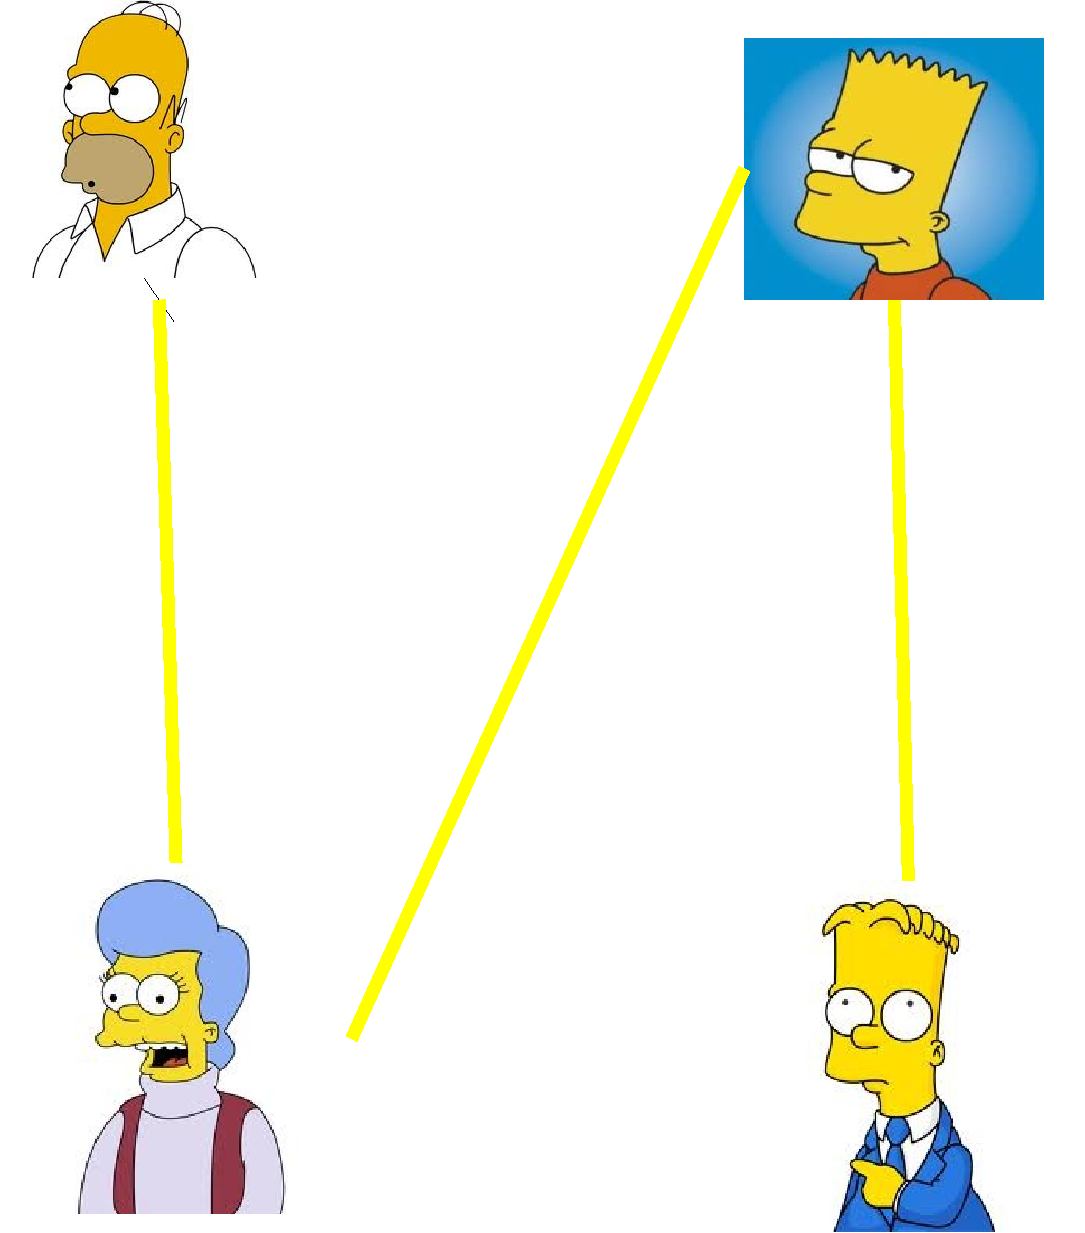
\includegraphics[width=0.6\textwidth]{figures/example.pdf}
%	\end{figure}
%}

%---------------------slide--------------------%
\section{Introduction and background}
\frame
{
	\frametitle{Matching}
	
	\uncover<1>{
	\begin{description}
		\item[Matching in a graph] is a set of edges, no two of which meet at a common vertex.
	\end{description}
	
	\begin{center}
		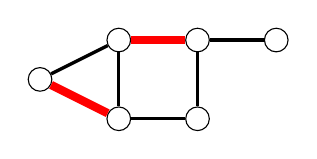
\begin{tikzpicture}[scale=0.5]
			\tikzstyle{Flower}	= [circle, fill=white, minimum size=4mm, inner sep=0pt]
			\tikzstyle{Vertex} 	= [circle, draw, solid,  fill=white, minimum size=3mm, inner sep=0pt]
			\tikzstyle{OUT}		= [fill = white]
			\tikzstyle{IN}		= [fill = black]
			\tikzstyle{Exposed}	= [dashed, blue, OUT]
			\tikzstyle{MC}		= [line width=3pt]
			\tikzstyle{NM}		= [very thick, black]
			
			\foreach \x/\y in {0/1, 2/0, 2/2, 4/0, 4/2, 6/2}
				\node (v\x\y) at (\x, \y) [Vertex] {};
			
			\foreach \a/\b/\c/\d in {0/1/2/2, 2/2/2/0, 2/0/4/0, 4/0/4/2, 4/2/6/2}
				\draw [-] (v\a\b) to (v\c\d) [NM];
			\foreach \a/\b/\c/\d in {0/1/2/0, 2/2/4/2}
				\draw [-] (v\a\b) to (v\c\d) [MC][red];
		\end{tikzpicture}
	\end{center}
	}
	%\pause
	\uncover<2>{
	\begin{description}
		\item[Maximum matching] is a matching of maximum cardinality.
	\end{description}
	
	\begin{center}
		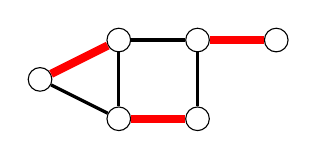
\begin{tikzpicture}[scale=0.5]
			\tikzstyle{Flower}	= [circle, fill=white, minimum size=4mm, inner sep=0pt]
			\tikzstyle{Vertex} 	= [circle, draw, solid,  fill=white, minimum size=3mm, inner sep=0pt]
			\tikzstyle{OUT}		= [fill = white]
			\tikzstyle{IN}		= [fill = black]
			\tikzstyle{Exposed}	= [dashed, blue, OUT]
			\tikzstyle{MC}		= [line width=3pt]
			\tikzstyle{NM}		= [very thick, black]
			
			\foreach \x/\y in {0/1, 2/0, 2/2, 4/0, 4/2, 6/2}
				\node (v\x\y) at (\x, \y) [Vertex] {};
			
			\foreach \a/\b/\c/\d in {0/1/2/0, 2/2/2/0, 2/2/4/2, 4/0/4/2}
				\draw [-] (v\a\b) to (v\c\d) [NM];
			\foreach \a/\b/\c/\d in {0/1/2/2, 2/0/4/0, 4/2/6/2}
				\draw [-] (v\a\b) to (v\c\d) [MC][red];
		\end{tikzpicture}
	\end{center}}
}

%---------------------slide--------------------%
\frame
{
	\frametitle{Question}
	
	\huge{Why do we want to study matching problems?}
	
}

%---------------------slide--------------------%
\frame
{
	\frametitle{A lot of applications}
	Job recruitment process.
	
	\begin{figure}[htb]
	\centering
	
\includegraphics[width=0.6\textwidth]{figures/mc.pdf}
	\end{figure}
}

%---------------------slide--------------------%
\frame
{
	\frametitle{A lot of applications}
	Then someone is not happy.
	
	\begin{figure}[htb]
	\centering
	\includegraphics[width=0.6\textwidth]{figures/mc22.pdf}
	\end{figure}
}

%---------------------slide--------------------%
\frame
{
	\frametitle{A lot of applications}
	Everyone is happy now.
	
	\begin{figure}[htb]
	\centering
	\includegraphics[width=0.6\textwidth]{figures/mc33.pdf}
	\end{figure}
}

%---------------------slide--------------------%
\frame
{
	\frametitle{Question}
	
	\huge{You don't want to do it manually.}
	
	\bigskip
	
	\huge{So, how can you find the maximum matching?}
	
}

%---------------------slide--------------------%
\frame
{
	\frametitle{First try: greedy method}
	
	\begin{overlayarea}{\textwidth}{1cm}
	\only<1>{
	Enumerate every edge, if both end points are not covered by the matching, add the edge to the matching.
	}
	\only<2>{
	\huge{How to improve the matching?}
	}
	\end{overlayarea}
	
	\begin{center}
		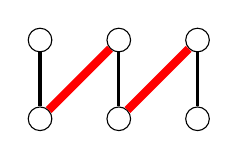
\begin{tikzpicture}
			\tikzstyle{Flower}	= [circle, fill=white, minimum size=4mm, inner sep=0pt]
			\tikzstyle{Vertex} 	= [circle, draw, solid,  fill=white, minimum size=3mm, inner sep=0pt]
			\tikzstyle{OUT}		= [fill = white]
			\tikzstyle{IN}		= [fill = black]
			\tikzstyle{Exposed}	= [dashed, blue, OUT]
			\tikzstyle{MC}		= [line width=3pt, red]
			\tikzstyle{NM}		= [very thick, black]
			
			\node (v0) at (0,0) [Vertex] {};
			\node (v1) at (1,0) [Vertex] {};
			\node (v2) at (0,1) [Vertex] {};
			\node (v3) at (1,1) [Vertex] {};
			\node (v4) at (2,0) [Vertex] {};
			\node (v5) at (2,1) [Vertex] {};
			
			\draw [-] (v0) to (v2) [NM];
			\draw [-] (v1) to (v3) [NM];
			\draw [-] (v0) to (v3) [MC];
			\draw [-] (v4) to (v5) [NM];
			\draw [-] (v1) to (v5) [MC];
			
		\end{tikzpicture}
	\end{center}
	
	\begin{overlayarea}{\textwidth}{1cm}
	\only<1>{
	Not always work. May reach local optimum (\alert{maximal} matching).
	}
	\end{overlayarea}
}

%---------------------slide--------------------%
\frame
{
	\frametitle{Augment the matching}
	
	\begin{overlayarea}{\textwidth}{1cm}
	If we flip the edges...
	\end{overlayarea}
	
	%\bigskip
	
	\begin{center}
		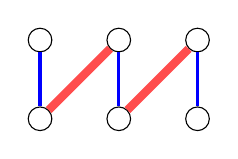
\begin{tikzpicture}
			\tikzstyle{Flower}	= [circle, fill=white, minimum size=4mm, inner sep=0pt]
			\tikzstyle{Vertex} 	= [circle, draw, solid,  fill=white, minimum size=3mm, inner sep=0pt]
			\tikzstyle{OUT}		= [fill = white]
			\tikzstyle{IN}		= [fill = black]
			\tikzstyle{Exposed}	= [dashed, blue, OUT]
			\tikzstyle{MC}		= [line width=3pt, opacity=0.7, red]
			\tikzstyle{NM}		= [very thick, blue]
			
			\node (v0) at (0,0) [Vertex] {};
			\node (v1) at (1,0) [Vertex] {};
			\node (v2) at (0,1) [Vertex] {};
			\node (v3) at (1,1) [Vertex] {};
			\node (v4) at (2,0) [Vertex] {};
			\node (v5) at (2,1) [Vertex] {};
			
			\draw [-] (v0) to (v2) [NM];
			\draw [-] (v1) to (v3) [NM];
			\draw [-] (v0) to (v3) [MC];
			\draw [-] (v4) to (v5) [NM];
			\draw [-] (v1) to (v5) [MC];
			
		\end{tikzpicture}
	\end{center}
	
	\begin{overlayarea}{\textwidth}{1cm}
 
 	\end{overlayarea}
}

%---------------------slide--------------------%
\frame
{
	\frametitle{Augment the matching}
	
	\begin{overlayarea}{\textwidth}{1cm}
	Seems we have found a way to improve the matching!
	\end{overlayarea}
	
	\begin{center}
		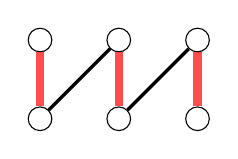
\begin{tikzpicture}
			\tikzstyle{Flower}	= [circle, fill=white, minimum size=4mm, inner sep=0pt]
			\tikzstyle{Vertex} 	= [circle, draw, solid,  fill=white, minimum size=3mm, inner sep=0pt]
			\tikzstyle{OUT}		= [fill = white]
			\tikzstyle{IN}		= [fill = black]
			\tikzstyle{Exposed}	= [dashed, blue, OUT]
			\tikzstyle{MC}		= [very thick, black]
			\tikzstyle{NM}		= [line width=3pt, opacity=0.7, red]
			
			\node (v0) at (0,0) [Vertex] {};
			\node (v1) at (1,0) [Vertex] {};
			\node (v2) at (0,1) [Vertex] {};
			\node (v3) at (1,1) [Vertex] {};
			\node (v4) at (2,0) [Vertex] {};
			\node (v5) at (2,1) [Vertex] {};
			
			\draw [-] (v0) to (v2) [NM];
			\draw [-] (v1) to (v3) [NM];
			\draw [-] (v0) to (v3) [MC];
			\draw [-] (v4) to (v5) [NM];
			\draw [-] (v1) to (v5) [MC];
		\end{tikzpicture}
	\end{center}
	
	\begin{overlayarea}{\textwidth}{1cm}
	Then we want to generalize the idea.
	\end{overlayarea}	
}

%---------------------slide--------------------%
\frame
{
	\frametitle{Exposed vertex}
	
	\begin{overlayarea}{\textwidth}{1cm}
	\begin{description}
		\item[Exposed(free) vertex] is a vertex that is not incident with any edge in the matching $M$
	\end{description}
	\end{overlayarea}
	
	\begin{center}
		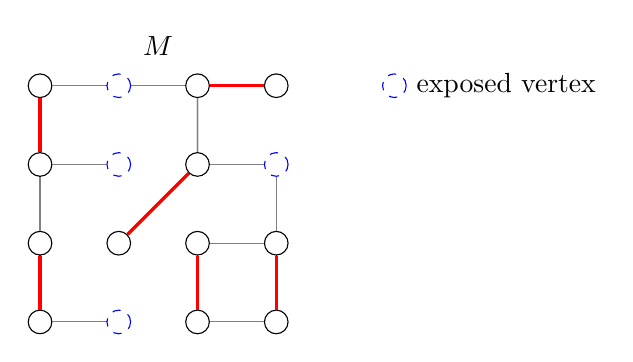
\begin{tikzpicture}
			\tikzstyle{Flower}	= [circle, fill=white, minimum size=4mm, inner sep=0pt]
			\tikzstyle{Vertex} 	= [circle, draw, solid,  fill=white, minimum size=3mm, inner sep=0pt]
			\tikzstyle{OUT}		= [fill = white]
			\tikzstyle{IN}		= [fill = black]
			\tikzstyle{Exposed}	= [dashed, blue, OUT]
			\tikzstyle{MC}		= [very thick, black]
			\tikzstyle{NM}		= [gray]
			
			
			\draw (2,0) -- (3,0) -- (3,1) -- (2,1) -- cycle;
			\draw (1,1) -- (2,2) -- (2,3) -- (3,3);
			\draw (1,0) -- (0,0) -- (0,1) -- (0,2) -- (0,3) -- (1,3);
			
			\draw (1.5, 3.5) node {$M$};
			\foreach \x/\y in {0/0, 2/0, 3/0, 0/1, 1/1, 2/1, 3/1, 0/2, 2/2, 0/3, 2/3, 3/3}
				\node (v\x\y) at (\x, \y) [Vertex] {};
			\foreach \x/\y in {1/0, 1/2, 3/2, 1/3}
				\node (v\x\y) at (\x, \y) [Vertex][Exposed] {};
			\foreach \a/\b/\c/\d in {0/0/1/0, 0/2/1/2, 2/0/3/0, 2/1/3/1, 2/2/3/2, 2/2/2/3, 2/0/2/1, 3/0/3/1, 0/1/0/2, 1/1/2/2, 0/3/1/3, 2/3/3/3, 1/3/2/3, 3/1/3/2, 0/0/0/1, 0/2/0/3}
				\draw [-] (v\a\b) to (v\c\d) [NM];
			\foreach \a/\b/\c/\d in {2/0/2/1, 3/0/3/1, 0/0/0/1, 1/1/2/2, 0/2/0/3, 2/3/3/3}
				\draw [-] (v\a\b) to (v\c\d) [MC][red];
			
			\node at (4.5, 3) [Vertex][Exposed][label=right:exposed vertex] {};
		\end{tikzpicture}
	\end{center}
	
	\begin{overlayarea}{\textwidth}{1cm}
	\end{overlayarea}
}

%---------------------slide--------------------%
\frame
{
	\frametitle{Alternating path}
	
	\begin{overlayarea}{\textwidth}{1cm}
	\begin{description}
		\item[Alternating path] is a path whose edges are alternately in $M$ and $\overline{M}$
	\end{description}
	\end{overlayarea}
		
	\begin{center}
		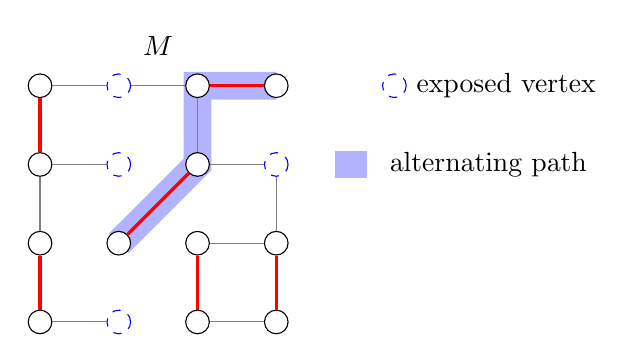
\begin{tikzpicture}
			\tikzstyle{Flower}	= [circle, fill=white, minimum size=4mm, inner sep=0pt]
			\tikzstyle{Vertex} 	= [circle, draw, solid,  fill=white, minimum size=3mm, inner sep=0pt]
			\tikzstyle{OUT}		= [fill = white]
			\tikzstyle{IN}		= [fill = black]
			\tikzstyle{Exposed}	= [dashed, blue, OUT]
			\tikzstyle{MC}		= [very thick, black]
			\tikzstyle{NM}		= [gray]
			
			\draw (1,1) -- (2,2) -- (2,3) -- (3,3) [line width=10pt, blue, opacity=0.3];
			
			\draw (1.5, 3.5) node {$M$};
			\foreach \x/\y in {0/0, 2/0, 3/0, 0/1, 1/1, 2/1, 3/1, 0/2, 2/2, 0/3, 2/3, 3/3}
				\node (v\x\y) at (\x, \y) [Vertex] {};
			\foreach \x/\y in {1/0, 1/2, 3/2, 1/3}
				\node (v\x\y) at (\x, \y) [Vertex][Exposed] {};
			\foreach \a/\b/\c/\d in {0/0/1/0, 0/2/1/2, 2/0/3/0, 2/1/3/1, 2/2/3/2, 2/2/2/3, 2/0/2/1, 3/0/3/1, 0/1/0/2, 1/1/2/2, 0/3/1/3, 2/3/3/3, 1/3/2/3, 3/1/3/2, 0/0/0/1, 0/2/0/3}
				\draw [-] (v\a\b) to (v\c\d) [NM];
			\foreach \a/\b/\c/\d in {2/0/2/1, 3/0/3/1, 0/0/0/1, 1/1/2/2, 0/2/0/3, 2/3/3/3}
				\draw [-] (v\a\b) to (v\c\d) [MC][red];
			
			\node at (4.5, 3) [Vertex][Exposed][label=right:exposed vertex] {};
			\draw (3.75,2) -- (4.15,2) [line width=10pt, blue, opacity=0.3] node [right, black, opacity=1]{alternating path};
		\end{tikzpicture}
	\end{center}
	
	\begin{overlayarea}{\textwidth}{1cm}
	\end{overlayarea}
}

%---------------------slide--------------------%
\frame
{
	\frametitle{Augmenting path}
	
	\begin{overlayarea}{\textwidth}{1cm}
	\begin{description}
		\item[Augmenting path] is a simple alternating path between exposed vertices
	\end{description}
	\end{overlayarea}
	
	\begin{center}
		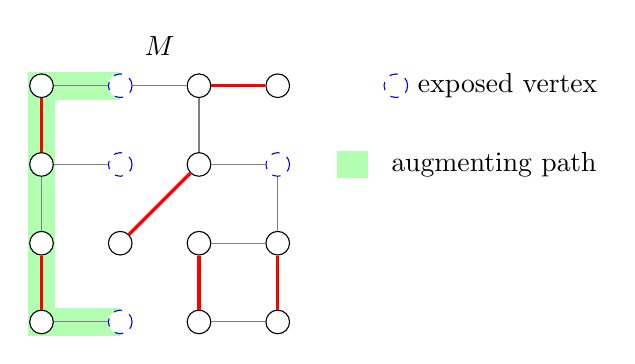
\begin{tikzpicture}
			\tikzstyle{Flower}	= [circle, fill=white, minimum size=4mm, inner sep=0pt]
			\tikzstyle{Vertex} 	= [circle, draw, solid,  fill=white, minimum size=3mm, inner sep=0pt]
			\tikzstyle{OUT}		= [fill = white]
			\tikzstyle{IN}		= [fill = black]
			\tikzstyle{Exposed}	= [dashed, blue, OUT]
			\tikzstyle{MC}		= [very thick, black]
			\tikzstyle{NM}		= [gray]
			
			\draw (1,0) -- (0,0) -- (0,1) -- (0,2) -- (0,3) -- (1,3) [line width=10pt, green, opacity=0.3];
			
			\draw (1.5, 3.5) node {$M$};
			\foreach \x/\y in {0/0, 2/0, 3/0, 0/1, 1/1, 2/1, 3/1, 0/2, 2/2, 0/3, 2/3, 3/3}
				\node (v\x\y) at (\x, \y) [Vertex] {};
			\foreach \x/\y in {1/0, 1/2, 3/2, 1/3}
				\node (v\x\y) at (\x, \y) [Vertex][Exposed] {};
			\foreach \a/\b/\c/\d in {0/0/1/0, 0/2/1/2, 2/0/3/0, 2/1/3/1, 2/2/3/2, 2/2/2/3, 2/0/2/1, 3/0/3/1, 0/1/0/2, 1/1/2/2, 0/3/1/3, 2/3/3/3, 1/3/2/3, 3/1/3/2, 0/0/0/1, 0/2/0/3}
				\draw [-] (v\a\b) to (v\c\d) [NM];
			\foreach \a/\b/\c/\d in {2/0/2/1, 3/0/3/1, 0/0/0/1, 1/1/2/2, 0/2/0/3, 2/3/3/3}
				\draw [-] (v\a\b) to (v\c\d) [MC][red];
			
			\node at (4.5, 3) [Vertex][Exposed][label=right:exposed vertex] {};
			\draw (3.75,2) -- (4.15,2) [line width=10pt, green, opacity=0.3] node [right, black, opacity=1]{augmenting path};
		\end{tikzpicture}
	\end{center}
	
	\begin{overlayarea}{\textwidth}{1cm}
	\end{overlayarea}
}

%---------------------slide--------------------%
\frame
{
	\frametitle{Augmenting path}
	
	\begin{overlayarea}{\textwidth}{1cm}
	\large{
	We can find a larger matching in the augmenting path!
	}
	\end{overlayarea}
	
	\begin{center}
		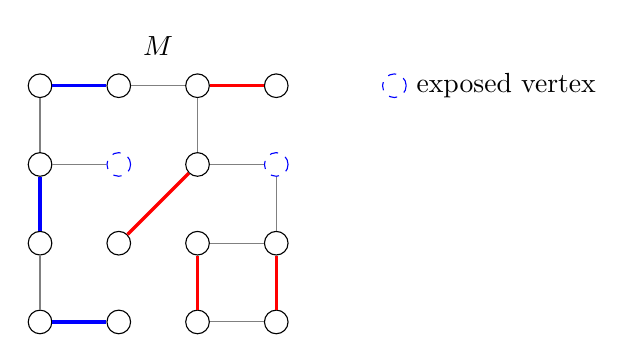
\begin{tikzpicture}
			\tikzstyle{Flower}	= [circle, fill=white, minimum size=4mm, inner sep=0pt]
			\tikzstyle{Vertex} 	= [circle, draw, solid,  fill=white, minimum size=3mm, inner sep=0pt]
			\tikzstyle{OUT}		= [fill = white]
			\tikzstyle{IN}		= [fill = black]
			\tikzstyle{Exposed}	= [dashed, blue, OUT]
			\tikzstyle{MC}		= [very thick, black]
			\tikzstyle{NM}		= [gray]
						
			\draw (1.5, 3.5) node {$M$};
			\foreach \x/\y in {1/0, 1/3, 0/0, 2/0, 3/0, 0/1, 1/1, 2/1, 3/1, 0/2, 2/2, 0/3, 2/3, 3/3}
				\node (v\x\y) at (\x, \y) [Vertex] {};
			\foreach \x/\y in {1/2, 3/2}
				\node (v\x\y) at (\x, \y) [Vertex][Exposed] {};
			\foreach \a/\b/\c/\d in {0/2/0/3, 0/0/0/1, 0/0/1/0, 0/2/1/2, 2/0/3/0, 2/1/3/1, 2/2/3/2, 2/2/2/3, 2/0/2/1, 3/0/3/1, 0/1/0/2, 1/1/2/2, 0/3/1/3, 2/3/3/3, 1/3/2/3, 3/1/3/2, 0/0/0/1, 0/2/0/3}
				\draw [-] (v\a\b) to (v\c\d) [NM];
			\foreach \a/\b/\c/\d in {2/0/2/1, 3/0/3/1, 1/1/2/2, 2/3/3/3}
				\draw [-] (v\a\b) to (v\c\d) [MC][red];
			
			\draw (v00) -- (v10) [MC][blue];
			\draw (v01) -- (v02) [MC][blue];
			\draw (v03) -- (v13) [MC][blue];
			
			\node at (4.5, 3) [Vertex][Exposed][label=right:exposed vertex] {};
		\end{tikzpicture}
	\end{center}
	
	\begin{overlayarea}{\textwidth}{1cm}
	This operation is called \alert{symmetric difference} $\oplus$.
	\end{overlayarea}
}

%---------------------slide--------------------%
\frame
{
	\frametitle{Symmetric difference}
	\begin{description}
		\item[Symmetric difference] of two sets $D$ and $E$ is defined as $D \oplus E = (D - E) \cup (E - D)$
	\end{description}
	
	\begin{center}
	\begin{figure}[h]
		\hfill
		\centering
		\begin{minipage}[c]{.45\textwidth}
		\centering
		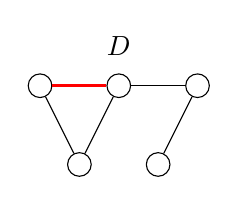
\begin{tikzpicture}
			\tikzstyle{Flower}	= [circle, fill=white, minimum size=4mm, inner sep=0pt]
			\tikzstyle{Vertex} 	= [circle, draw, solid,  fill=white, minimum size=3mm, inner sep=0pt]
			\tikzstyle{OUT}		= [fill = white]
			\tikzstyle{IN}		= [fill = black]
			\tikzstyle{Exposed}	= [dashed, blue, OUT]
			\tikzstyle{MC}		= [very thick]
			\tikzstyle{NM}		= [black]
			
			\draw (1, 1.5) node {$D$};
			\node (v1) at (0, 1) [Vertex] {};
			\node (v2) at (0.5, 0) [Vertex] {};
			\node (v3) at (1, 1) [Vertex] {};
			\node (v4) at (1.5, 0) [Vertex] {};
			\node (v5) at (2, 1) [Vertex] {};
			
			\draw [-] (v1) to (v2) [NM];
			\draw [-] (v2) to (v3) [NM];
			\draw [-] (v3) to (v5) [NM];
			\draw [-] (v4) to (v5) [NM];
			
			\draw [-] (v1) to (v3) [MC][red];
		\end{tikzpicture}
		\end{minipage}
		\hfill
		\centering
		\begin{minipage}[c]{.45\textwidth}
		\centering
		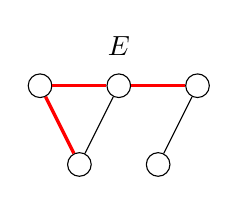
\begin{tikzpicture}
			\tikzstyle{Flower}	= [circle, fill=white, minimum size=4mm, inner sep=0pt]
			\tikzstyle{Vertex} 	= [circle, draw, solid,  fill=white, minimum size=3mm, inner sep=0pt]
			\tikzstyle{OUT}		= [fill = white]
			\tikzstyle{IN}		= [fill = black]
			\tikzstyle{Exposed}	= [dashed, blue, OUT]
			\tikzstyle{MC}		= [very thick]
			\tikzstyle{NM}		= [black]
			
			\draw (1, 1.5) node {$E$};
			\node (v1) at (0, 1) [Vertex] {};
			\node (v2) at (0.5, 0) [Vertex] {};
			\node (v3) at (1, 1) [Vertex] {};
			\node (v4) at (1.5, 0) [Vertex] {};
			\node (v5) at (2, 1) [Vertex] {};
			
			\draw [-] (v2) to (v3) [NM];
			\draw [-] (v4) to (v5) [NM];
			
			\draw [-] (v1) to (v3) [MC][red];
			\draw [-] (v1) to (v2) [MC][red];
			\draw [-] (v3) to (v5) [MC][red];
		\end{tikzpicture}
		\end{minipage}
		\hfill
	\end{figure}
	\end{center}
	
	\begin{center}
	\begin{figure}[h]
		\centering
		\begin{minipage}[c]{.45\textwidth}
		\centering
		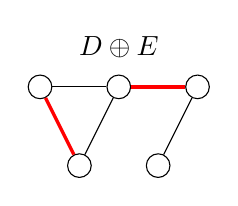
\begin{tikzpicture}
			\tikzstyle{Flower}	= [circle, fill=white, minimum size=4mm, inner sep=0pt]
			\tikzstyle{Vertex} 	= [circle, draw, solid,  fill=white, minimum size=3mm, inner sep=0pt]
			\tikzstyle{OUT}		= [fill = white]
			\tikzstyle{IN}		= [fill = black]
			\tikzstyle{Exposed}	= [dashed, blue, OUT]
			\tikzstyle{MC}		= [very thick]
			\tikzstyle{NM}		= [black]
			
			\draw (1, 1.5) node {$D \oplus E$};
			\node (v1) at (0, 1) [Vertex] {};
			\node (v2) at (0.5, 0) [Vertex] {};
			\node (v3) at (1, 1) [Vertex] {};
			\node (v4) at (1.5, 0) [Vertex] {};
			\node (v5) at (2, 1) [Vertex] {};
			
			\draw [-] (v2) to (v3) [NM];
			\draw [-] (v4) to (v5) [NM];
			\draw [-] (v1) to (v3) [NM];
			
			\draw [-] (v1) to (v2) [MC][red];
			\draw [-] (v3) to (v5) [MC][red];
		\end{tikzpicture}
		\end{minipage}
	\end{figure}
	\end{center}
	
	The result of the symmetric difference between a matching and an augmenting path on the graph is a larger matching.
}

%---------------------slide--------------------%
\frame
{
	\frametitle{Intuition}
	
	\huge{
	Then our algorithm can try to find augmenting paths to improve the known mathcing.
	}
	
}

%---------------------slide--------------------%
\frame
{
	\frametitle{Question}
	
	\huge{
	Can we stop when there is no augmenting paths?	
	
	\bigskip
	
	What is the optimality condition for the algorithm to terminate?
	}
	
}

%---------------------slide--------------------%
\frame
{
	\frametitle{Answer}
	
	\huge{Berge theorem says if there is no augmenting path, we can stop!}
	
}

%%---------------------slide--------------------%
%\frame
%{
%	\frametitle{Alternating path}
%	
%	\begin{beamercolorbox}[sep=1em,wd=11cm]{postit}
%		For any two matchings $M_{1}$ and $M_{2}$ in graph $G$, the components of the graph formed by $M_{1} \oplus M_{2}$ are paths and circuits which are alternating for $M_{1}$ and $M_{2}$. Each path end-point is exposed for either $M_{1}$ or $M_{2}$.
%	\end{beamercolorbox}
%	
%	\begin{center}
%	\begin{figure}[h]
%		\hfill
%		\centering
%		\begin{minipage}[c]{.45\textwidth}
%		\centering
%		\begin{tikzpicture}
%			\tikzstyle{Flower}	= [circle, fill=white, minimum size=4mm, inner sep=0pt]
%			\tikzstyle{Vertex} 	= [circle, draw, solid,  fill=white, minimum size=3mm, inner sep=0pt]
%			\tikzstyle{OUT}		= [fill = white]
%			\tikzstyle{IN}		= [fill = black]
%			\tikzstyle{Exposed1}	= [dashed, blue, OUT]
%			\tikzstyle{MC}		= [very thick]
%			\tikzstyle{NM}		= [black]
%			
%			\draw (1, 1.5) node {$M_{1}$};
%			\node (v1) at (0, 1) [Vertex] {};
%			\node (v2) at (0.5, 0) [Vertex][Exposed1] {};
%			\node (v3) at (1, 1) [Vertex] {};
%			\node (v4) at (1.5, 0) [Vertex][Exposed1] {};
%			\node (v5) at (2, 1) [Vertex][Exposed1] {};
%			
%			\draw [-] (v1) to (v2) [NM];
%			\draw [-] (v2) to (v3) [NM];
%			\draw [-] (v3) to (v5) [NM];
%			\draw [-] (v4) to (v5) [NM];
%			
%			\draw [-] (v1) to (v3) [MC][red];
%		\end{tikzpicture}
%		\end{minipage}
%		\hfill
%		\centering
%		\begin{minipage}[c]{.45\textwidth}
%		\centering
%		\begin{tikzpicture}
%			\tikzstyle{Flower}	= [circle, fill=white, minimum size=4mm, inner sep=0pt]
%			\tikzstyle{Vertex} 	= [circle, draw, solid,  fill=white, minimum size=3mm, inner sep=0pt]
%			\tikzstyle{OUT}		= [fill = white]
%			\tikzstyle{IN}		= [fill = black]
%			\tikzstyle{Exposed2}	= [dashed, green, OUT]
%			\tikzstyle{MC}		= [very thick]
%			\tikzstyle{NM}		= [black]
%			
%			\draw (1, 1.5) node {$M_{2}$};
%			\node (v1) at (0, 1) [Vertex] {};
%			\node (v2) at (0.5, 0) [Vertex] {};
%			\node (v3) at (1, 1) [Vertex] {};
%			\node (v4) at (1.5, 0) [Vertex][Exposed2] {};
%			\node (v5) at (2, 1) [Vertex] {};
%			
%			\draw [-] (v2) to (v3) [NM];
%			\draw [-] (v4) to (v5) [NM];
%			\draw [-] (v1) to (v3) [NM];
%			
%			\draw [-] (v1) to (v2) [MC][blue];
%			\draw [-] (v3) to (v5) [MC][blue];
%		\end{tikzpicture}
%		\end{minipage}
%		\hfill
%	\end{figure}
%	\end{center}
%	
%	\begin{center}
%	\begin{figure}[h]
%		\centering
%		\begin{minipage}[c]{.45\textwidth}
%		\centering
%		\begin{tikzpicture}
%			\tikzstyle{Flower}	= [circle, fill=white, minimum size=4mm, inner sep=0pt]
%			\tikzstyle{Vertex} 	= [circle, draw, solid,  fill=white, minimum size=3mm, inner sep=0pt]
%			\tikzstyle{OUT}		= [fill = white]
%			\tikzstyle{IN}		= [fill = black]
%			\tikzstyle{Exposed1}	= [dashed, blue, OUT]
%			\tikzstyle{Exposed2}	= [dashed, green, OUT]
%			\tikzstyle{MC}		= [very thick]
%			\tikzstyle{NM}		= [black]
%			
%			\draw (1, 1.5) node {$M_{1} \oplus M_{2}$};
%			\node (v1) at (0, 1) [Vertex] {};
%			\node (v2) at (0.5, 0) [Vertex][Exposed1] {};
%			\node (v3) at (1, 1) [Vertex] {};
%			\node (v4) at (1.5, 0) [Vertex] {};
%			\node (v5) at (2, 1) [Vertex][Exposed1] {};
%			
%			\draw [-] (v2) to (v3) [NM];
%			\draw [-] (v4) to (v5) [NM];
%			
%			\draw [-] (v1) to (v2) [MC][blue];
%			\draw [-] (v1) to (v3) [MC][red];
%			\draw [-] (v3) to (v5) [MC][blue];
%		\end{tikzpicture}
%		\end{minipage}
%	\end{figure}
%	\end{center}
%}
%
%%---------------------slide--------------------%
%\frame
%{
%	\frametitle{Augmenting path}
%	\begin{beamercolorbox}[sep=1em,wd=11cm]{postit}
%		$A$ is an augmenting path in $(G, M)$ . $M \oplus A$ is a matching of $G$ larger than $M$ by one.
%	\end{beamercolorbox}
%	
%	\begin{center}
%	\begin{figure}
%		\hfill
%		\centering
%		\begin{minipage}[c]{.45\textwidth}
%		\centering
%		\begin{tikzpicture}
%			\tikzstyle{Flower}	= [circle, fill=white, minimum size=4mm, inner sep=0pt]
%			\tikzstyle{Vertex} 	= [circle, draw, solid,  fill=white, minimum size=3mm, inner sep=0pt]
%			\tikzstyle{OUT}		= [fill = white]
%			\tikzstyle{IN}		= [fill = black]
%			\tikzstyle{Exposed1}	= [dashed, blue, OUT]
%			\tikzstyle{MC}		= [very thick]
%			\tikzstyle{NM}		= [black]
%			
%			\draw (1, 1.5) node {$M$};
%			\node (v1) at (0, 1) [Vertex] {};
%			\node (v2) at (0.5, 0) [Vertex][Exposed1] {};
%			\node (v3) at (1, 1) [Vertex] {};
%			\node (v4) at (1.5, 0) [Vertex][Exposed1] {};
%			\node (v5) at (2, 1) [Vertex][Exposed1] {};
%			
%			\draw [-] (v1) to (v2) [NM];
%			\draw [-] (v2) to (v3) [NM];
%			\draw [-] (v3) to (v5) [NM];
%			\draw [-] (v4) to (v5) [NM];
%			
%			\draw [-] (v1) to (v3) [MC][red];
%		\end{tikzpicture}
%		\end{minipage}
%		\hfill
%		\centering
%		\begin{minipage}[c]{.45\textwidth}
%		\centering
%		\begin{tikzpicture}
%			\tikzstyle{Flower}	= [circle, fill=white, minimum size=4mm, inner sep=0pt]
%			\tikzstyle{Vertex} 	= [circle, draw, solid,  fill=white, minimum size=3mm, inner sep=0pt]
%			\tikzstyle{OUT}		= [fill = white]
%			\tikzstyle{IN}		= [fill = black]
%			\tikzstyle{Exposed1}	= [dashed, blue, OUT]
%			\tikzstyle{MC}		= [very thick]
%			\tikzstyle{NM}		= [black]
%			
%			\draw (1, 1.5) node {$A$};
%			\node (v1) at (0, 1) [Vertex] {};
%			\node (v2) at (0.5, 0) [Vertex][Exposed1] {};
%			\node (v3) at (1, 1) [Vertex] {};
%			\node (v4) at (1.5, 0) [Vertex][Exposed1] {};
%			\node (v5) at (2, 1) [Vertex][Exposed1] {};
%			
%			\draw [-] (v1) to (v2) [NM];
%			\draw [-] (v2) to (v3) [NM];
%			\draw [-] (v3) to (v5) [NM];
%			\draw [-] (v4) to (v5) [NM];
%			
%			\draw [-] (v1) to (v3) [MC][red];
%			
%			\draw (v2) -- (v1) -- (v3) -- (v5) [line width=10pt, green, opacity=0.3];
%		\end{tikzpicture}
%		\end{minipage}
%		\hfill
%	\end{figure}
%	\end{center}
%	
%	\begin{center}
%	\begin{figure}[h]
%		\centering
%		\begin{minipage}[c]{.45\textwidth}
%		\centering
%		\begin{tikzpicture}
%			\tikzstyle{Flower}	= [circle, fill=white, minimum size=4mm, inner sep=0pt]
%			\tikzstyle{Vertex} 	= [circle, draw, solid,  fill=white, minimum size=3mm, inner sep=0pt]
%			\tikzstyle{OUT}		= [fill = white]
%			\tikzstyle{IN}		= [fill = black]
%			\tikzstyle{Exposed1}	= [dashed, blue, OUT]
%			\tikzstyle{Exposed2}	= [dashed, green, OUT]
%			\tikzstyle{MC}		= [very thick]
%			\tikzstyle{NM}		= [black]
%			
%			\draw (1, 1.5) node {$M \oplus A$};
%			\node (v1) at (0, 1) [Vertex] {};
%			\node (v2) at (0.5, 0) [Vertex][Exposed1] {};
%			\node (v3) at (1, 1) [Vertex] {};
%			\node (v4) at (1.5, 0) [Vertex] {};
%			\node (v5) at (2, 1) [Vertex][Exposed1] {};
%			
%			\draw [-] (v2) to (v3) [NM];
%			\draw [-] (v4) to (v5) [NM];
%			\draw [-] (v1) to (v3) [NM];
%			
%			\draw [-] (v1) to (v2) [MC][red];
%			\draw [-] (v3) to (v5) [MC][red];
%		\end{tikzpicture}
%		\end{minipage}
%	\end{figure}
%	\end{center}
%}

%---------------------slide--------------------%
\frame
{
	\frametitle{Berge's theorem}
	
	\begin{block}{Theorem - Berge(1957)}
		$M$ is not a maximum matching if and only if there exists an augmenting path with respect to $M$
	\end{block}	
	
	\begin{itemize}
	{
		\item Proof:
		
		We have already seen that if there is an augmenting path we can find a larger matching. 
		
		\bigskip
		
		So we only need to prove if the matching is not maximum, there must exist an augmenting path.
	}
	\end{itemize}
	
}

%---------------------slide--------------------%
\frame
{
	\frametitle{Berge's theorem}
	
	\huge{If we have a larger matching, how to find an augmenting path?}
	
}

%---------------------slide--------------------%
\frame
{
	\frametitle{Berge's theorem}
	
	\large{
	Recall that we use $\oplus$ to find a larger matching.
	
	\bigskip
	
	Now we reverse the step. If we apply $\oplus$ between matching $M_{1}$ and a larger matching $M_{2}$, what do we get?
	}
}

%---------------------slide--------------------%
\frame
{
	\frametitle{Berge's theorem}
	
	The results are paths and circuits which are alternating for $M_{1}$ and $M_{2}$.
	
	\begin{center}
	\begin{figure}[scale=0.6,h]
		\hfill
		\centering
		\begin{minipage}[c]{.45\textwidth}
		\centering
		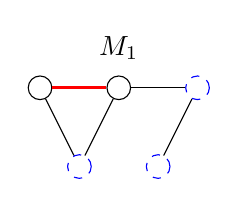
\begin{tikzpicture}
			\tikzstyle{Flower}	= [circle, fill=white, minimum size=4mm, inner sep=0pt]
			\tikzstyle{Vertex} 	= [circle, draw, solid,  fill=white, minimum size=3mm, inner sep=0pt]
			\tikzstyle{OUT}		= [fill = white]
			\tikzstyle{IN}		= [fill = black]
			\tikzstyle{Exposed1}	= [dashed, blue, OUT]
			\tikzstyle{MC}		= [very thick]
			\tikzstyle{NM}		= [black]
			
			\draw (1, 1.5) node {$M_{1}$};
			\node (v1) at (0, 1) [Vertex] {};
			\node (v2) at (0.5, 0) [Vertex][Exposed1] {};
			\node (v3) at (1, 1) [Vertex] {};
			\node (v4) at (1.5, 0) [Vertex][Exposed1] {};
			\node (v5) at (2, 1) [Vertex][Exposed1] {};
			
			\draw [-] (v1) to (v2) [NM];
			\draw [-] (v2) to (v3) [NM];
			\draw [-] (v3) to (v5) [NM];
			\draw [-] (v4) to (v5) [NM];
			
			\draw [-] (v1) to (v3) [MC][red];
		\end{tikzpicture}
		\end{minipage}
		\hfill
		\centering
		\begin{minipage}[c]{.45\textwidth}
		\centering
		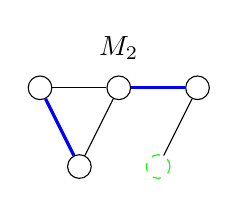
\begin{tikzpicture}
			\tikzstyle{Flower}	= [circle, fill=white, minimum size=4mm, inner sep=0pt]
			\tikzstyle{Vertex} 	= [circle, draw, solid,  fill=white, minimum size=3mm, inner sep=0pt]
			\tikzstyle{OUT}		= [fill = white]
			\tikzstyle{IN}		= [fill = black]
			\tikzstyle{Exposed2}	= [dashed, green, OUT]
			\tikzstyle{MC}		= [very thick]
			\tikzstyle{NM}		= [black]
			
			\draw (1, 1.5) node {$M_{2}$};
			\node (v1) at (0, 1) [Vertex] {};
			\node (v2) at (0.5, 0) [Vertex] {};
			\node (v3) at (1, 1) [Vertex] {};
			\node (v4) at (1.5, 0) [Vertex][Exposed2] {};
			\node (v5) at (2, 1) [Vertex] {};
			
			\draw [-] (v2) to (v3) [NM];
			\draw [-] (v4) to (v5) [NM];
			\draw [-] (v1) to (v3) [NM];
			
			\draw [-] (v1) to (v2) [MC][blue];
			\draw [-] (v3) to (v5) [MC][blue];
		\end{tikzpicture}
		\end{minipage}
		\hfill
	\end{figure}
	\end{center}
	
	\begin{center}
	\begin{figure}[h]
		\centering
		\begin{minipage}[c]{.45\textwidth}
		\centering
		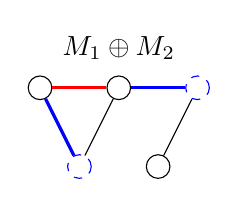
\begin{tikzpicture}
			\tikzstyle{Flower}	= [circle, fill=white, minimum size=4mm, inner sep=0pt]
			\tikzstyle{Vertex} 	= [circle, draw, solid,  fill=white, minimum size=3mm, inner sep=0pt]
			\tikzstyle{OUT}		= [fill = white]
			\tikzstyle{IN}		= [fill = black]
			\tikzstyle{Exposed1}	= [dashed, blue, OUT]
			\tikzstyle{Exposed2}	= [dashed, green, OUT]
			\tikzstyle{MC}		= [very thick]
			\tikzstyle{NM}		= [black]
			
			\draw (1, 1.5) node {$M_{1} \oplus M_{2}$};
			\node (v1) at (0, 1) [Vertex] {};
			\node (v2) at (0.5, 0) [Vertex][Exposed1] {};
			\node (v3) at (1, 1) [Vertex] {};
			\node (v4) at (1.5, 0) [Vertex] {};
			\node (v5) at (2, 1) [Vertex][Exposed1] {};
			
			\draw [-] (v2) to (v3) [NM];
			\draw [-] (v4) to (v5) [NM];
			
			\draw [-] (v1) to (v2) [MC][blue];
			\draw [-] (v1) to (v3) [MC][red];
			\draw [-] (v3) to (v5) [MC][blue];
		\end{tikzpicture}
		\end{minipage}
	\end{figure}
	\end{center}
	
	We have found alternating paths, which is very close to find augmenting paths!
}

%---------------------slide--------------------%
\frame
{
	\frametitle{Berge's theorem}
	
	
	\large{
	\uncover<1->{
	Since the matching $M_{2}$ is larger, there must be a component has one more edge in $M_{2}$ than in $M_{1}$.	
	}
	
	\bigskip
	
	\uncover<2->{
	This component is an augmenting path.
	}
	
	\bigskip
	
	\uncover<3->{	
	Why?
	}
	}
	
}

%---------------------slide--------------------%
\frame
{
	\frametitle{Berge's theorem}
	
	Because there are only four kinds of alternating paths. The only case when edges not in the matching are more than edges in the matching is an augmenting path!
	
	\begin{center}
	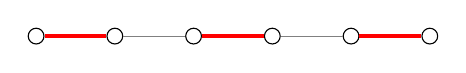
\begin{tikzpicture}
		\tikzstyle{Flower}	= [circle, fill=white, minimum size=2mm, inner sep=0pt]
		\tikzstyle{Vertex} 	= [circle, draw, solid,  fill=white, minimum size=2mm, inner sep=0pt]
		\tikzstyle{OUT}		= [fill = white]
		\tikzstyle{IN}		= [fill = black]
		\tikzstyle{Exposed}	= [dashed, OUT]
		\tikzstyle{MC}		= [very thick, red]
		\tikzstyle{NM}		= [gray]
		
		\node (v0) at (0,0) [Vertex] {};
		\node (v1) at (1,0) [Vertex] {};
		\node (v2) at (2,0) [Vertex] {};
		\node (v3) at (3,0) [Vertex] {};
		\node (v4) at (4,0) [Vertex] {};
		\node (v5) at (5,0) [Vertex] {};
		
		\draw [-] (v0) to (v1) [MC];
		\draw [-] (v1) to (v2) [NM];
		\draw [-] (v2) to (v3) [MC];
		\draw [-] (v3) to (v4) [NM];
		\draw [-] (v4) to (v5) [MC];
	\end{tikzpicture}
	\end{center}
	
	\begin{center}
	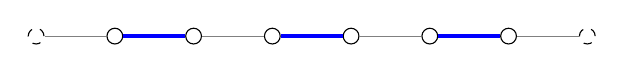
\begin{tikzpicture}
		\tikzstyle{Flower}	= [circle, fill=white, minimum size=2mm, inner sep=0pt]
		\tikzstyle{Vertex} 	= [circle, draw, solid,  fill=white, minimum size=2mm, inner sep=0pt]
		\tikzstyle{OUT}		= [fill = white]
		\tikzstyle{IN}		= [fill = black]
		\tikzstyle{Exposed}	= [dashed, OUT]
		\tikzstyle{MC}		= [very thick, blue]
		\tikzstyle{NM}		= [gray]
		
		\node (v0) at (0,0) [Vertex][Exposed] {};
		\node (v1) at (1,0) [Vertex] {};
		\node (v2) at (2,0) [Vertex] {};
		\node (v3) at (3,0) [Vertex] {};
		\node (v4) at (4,0) [Vertex] {};
		\node (v5) at (5,0) [Vertex] {};
		\node (v6) at (6,0) [Vertex] {};
		\node (v7) at (7,0) [Vertex][Exposed] {};
		
		\draw [-] (v0) to (v1) [NM];
		\draw [-] (v1) to (v2) [MC];
		\draw [-] (v2) to (v3) [NM];
		\draw [-] (v3) to (v4) [MC];
		\draw [-] (v4) to (v5) [NM];
		\draw [-] (v5) to (v6) [MC];
		\draw [-] (v6) to (v7) [NM];
	\end{tikzpicture}
	\end{center}
	
	\begin{center}
	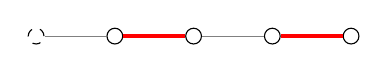
\begin{tikzpicture}
		\tikzstyle{Flower}	= [circle, fill=white, minimum size=2mm, inner sep=0pt]
		\tikzstyle{Vertex} 	= [circle, draw, solid,  fill=white, minimum size=2mm, inner sep=0pt]
		\tikzstyle{OUT}		= [fill = white]
		\tikzstyle{IN}		= [fill = black]
		\tikzstyle{Exposed}	= [dashed, OUT]
		\tikzstyle{MC}		= [very thick, red]
		\tikzstyle{NM}		= [gray]
		
		\node (v0) at (0,0) [Vertex][Exposed] {};
		\node (v1) at (1,0) [Vertex] {};
		\node (v2) at (2,0) [Vertex] {};
		\node (v3) at (3,0) [Vertex] {};
		\node (v4) at (4,0) [Vertex] {};
		
		\draw [-] (v0) to (v1) [NM];
		\draw [-] (v1) to (v2) [MC];
		\draw [-] (v2) to (v3) [NM];
		\draw [-] (v3) to (v4) [MC];
	\end{tikzpicture}
	\end{center}
	
	\begin{center}
	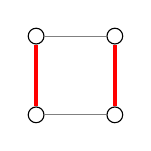
\begin{tikzpicture}
		\tikzstyle{Flower}	= [circle, fill=white, minimum size=2mm, inner sep=0pt]
		\tikzstyle{Vertex} 	= [circle, draw, solid,  fill=white, minimum size=2mm, inner sep=0pt]
		\tikzstyle{OUT}		= [fill = white]
		\tikzstyle{IN}		= [fill = black]
		\tikzstyle{Exposed}	= [dashed, OUT]
		\tikzstyle{MC}		= [very thick, red]
		\tikzstyle{NM}		= [gray]
		
		\node (v0) at (0,0) [Vertex] {};
		\node (v1) at (1,0) [Vertex] {};
		\node (v2) at (1,1) [Vertex] {};
		\node (v3) at (0,1) [Vertex] {};
		
		\draw [-] (v0) to (v1) [NM];
		\draw [-] (v1) to (v2) [MC];
		\draw [-] (v2) to (v3) [NM];
		\draw [-] (v3) to (v0) [MC];
	\end{tikzpicture}
	\end{center}
}

%---------------------slide--------------------%
\frame
{
	\frametitle{Algorithm}

	Then we have a general algorithm, which keeps finding augmenting paths and improving the matching until there is no more augmenting path.
	
	\begin{codebox}
	\Procname{$\proc{Maximum-Matching}(G)$}
	\li $M \gets \emptyset$ 
	\li \Repeat
	\li		\If there is an augmenting path $P$ with respect to $M$ 
	\li			\Then		       
					$M \gets M \oplus P$
			\End
	\li	\Until there isn't an augmenting path with respect to $M$
	\li \Return $M$
	\end{codebox}
}

%---------------------slide--------------------%
\frame
{
	\frametitle{Algorithm}

	\large{
	How can we perform the search for an augmenting path efficiently? By brute force, the search space could be \alert{exponential}.
	
	\bigskip
	
	And... what is an \alert{efficient} algorithm?
	}
}

%---------------------slide--------------------%
\frame
{
	\frametitle{Digression}

	\large{
	Edmonds defined that an efficient algorithm should have polynomial running time in this paper, which is earlier than Stephen Cook defined $\mathcal{P}$ and  $\mathcal{NP}$.
		
	}
}

%---------------------slide--------------------%
\frame
{
	\frametitle{Previous work: bipartite matching}
	A bipartite graph is a graph whose vertices can be divided into two disjoint sets $U$ and $V$ such that every edge connects a vertex in $U$ to one in $V$.
	
	\bigskip
	
	Equivalently, a bipartite graph is a graph that does \alert{not} contain any \alert{odd-length} cycles!
	
	\bigskip
	
	There are polynomial time algorithms for maximum matching on bipartite graphs!
	
	\begin{center}
		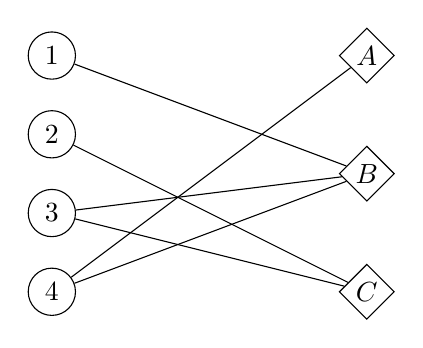
\begin{tikzpicture}
			\tikzstyle{Vertex} 	= [draw, solid,  fill=white, minimum size=6mm, inner sep=0pt]
			\tikzstyle{Exposed}	= []
			\tikzstyle{Boy}		= [circle]
			\tikzstyle{Girl}	= [diamond, minimum size=7mm]
			\tikzstyle{MC}		= [black]
			\tikzstyle{NM}		= [black]
			
			\node (b1) at (0,6) [Vertex][Boy][Exposed] {$1$};
			\node (b2) at (0,5) [Vertex][Boy][Exposed] {$2$};
			\node (b3) at (0,4) [Vertex][Boy] {$3$};
			\node (b4) at (0,3) [Vertex][Boy] {$4$};
			
			\node (ga) at (4,6.00) [Vertex][Girl][Exposed] {$A$};
			\node (gb) at (4,4.50) [Vertex][Girl] {$B$};
			\node (gc) at (4,3.00) [Vertex][Girl] {$C$};
			
			\draw [-] (b1) to (gb) [NM];
			\draw [-] (b2) to (gc) [NM];
			\draw [-] (b3) to (gb) [NM];
			\draw [-] (b3) to (gc) [MC];
			\draw [-] (b4) to (ga) [NM];
			\draw [-] (b4) to (gb) [MC];
		\end{tikzpicture}
	\end{center}
}

%---------------------slide--------------------%
\frame
{
	\frametitle{Find an augmenting path using BFS}
	
	\begin{overlayarea}{\textwidth}{1.5cm}
	We can use some greedy heuristic to find an initial matching. Then we start from an exposed vertex to grow an alternating tree, since the augmenting path is an alternating path.
	\end{overlayarea}
		
	\begin{center}
	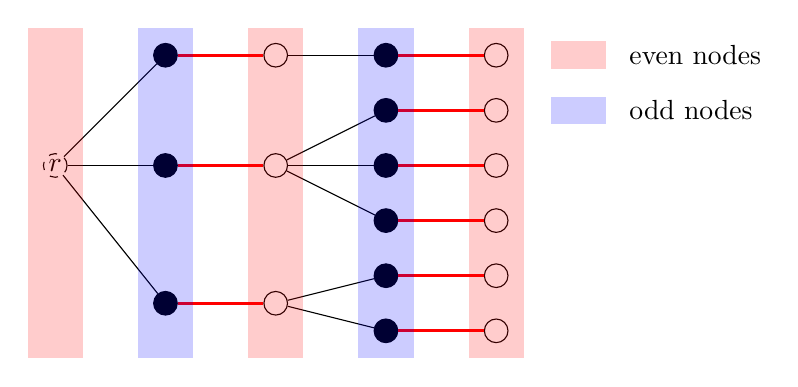
\begin{tikzpicture}[scale=0.7]
		\tikzstyle{Vertex} 	= [circle, draw, solid, fill=white, minimum size=3mm, inner sep=0pt]
		\tikzstyle{Exposed}	= [dashed]
		\tikzstyle{odd}	= [black]
		\tikzstyle{MC}		= [very thick, red]
		\tikzstyle{NM}		= [black]
			
		\node (v1) at (0, 0) [Vertex][Exposed] {$r$};
		\node (v2) at (2, 2) [Vertex][odd]{};
		\node (v3) at (2, 0) [Vertex][odd]{};
		\node (v4) at (2, -2.5) [Vertex][odd]{};
		\node (v5) at (4, 2) [Vertex]{};
		\node (v6) at (4, 0) [Vertex]{};
		\node (v7) at (4, -2.5) [Vertex]{};
		\node (v8) at (6, 2) [Vertex][odd]{};
		\node (v9) at (6, 1) [Vertex][odd]{};
		\node (v10) at (6, 0) [Vertex][odd]{};
		\node (v11) at (6, -1) [Vertex][odd]{};
		\node (v12) at (6, -2) [Vertex][odd]{};
		\node (v13) at (6, -3) [Vertex][odd]{};
		\node (v14) at (8, 2) [Vertex]{};
		\node (v15) at (8, 1) [Vertex]{};
		\node (v16) at (8, 0) [Vertex]{};
		\node (v17) at (8, -1) [Vertex]{};
		\node (v18) at (8, -2) [Vertex]{};
		\node (v19) at (8, -3) [Vertex]{};
			
		\draw [-] (v1) to (v2) [NM];
		\draw [-] (v1) to (v3) [NM];
		\draw [-] (v1) to (v4) [NM];
		\draw [-] (v2) to (v5) [MC];
		\draw [-] (v3) to (v6) [MC];
		\draw [-] (v4) to (v7) [MC];
		\draw [-] (v5) to (v8) [NM];
		\draw [-] (v6) to (v9) [NM];
		\draw [-] (v6) to (v10) [NM];
		\draw [-] (v6) to (v11) [NM];
		\draw [-] (v7) to (v12) [NM];
		\draw [-] (v7) to (v13) [NM];
		\draw [-] (v8) to (v14) [MC];
		\draw [-] (v9) to (v15) [MC];
		\draw [-] (v10) to (v16) [MC];
		\draw [-] (v11) to (v17) [MC];
		\draw [-] (v12) to (v18) [MC];
		\draw [-] (v13) to (v19) [MC];
		
		\fill[red, opacity = 0.2] (-0.5, 2.5) rectangle (0.5, -3.5);
		\fill[blue, opacity = 0.2] (2-0.5, 2.5) rectangle (2+0.5, -3.5);
		\fill[red, opacity = 0.2] (4-0.5, 2.5) rectangle (4+0.5, -3.5);
		\fill[blue, opacity = 0.2] (6-0.5, 2.5) rectangle (6+0.5, -3.5);
		\fill[red, opacity = 0.2] (8-0.5, 2.5) rectangle (8+0.5, -3.5);
		
		\draw (9,2) -- (10,2) [line width=10pt, red, opacity=0.2] node [right, black, opacity=1]{even nodes};
		\draw (9,1) -- (10,1) [line width=10pt, blue, opacity=0.2] node [right, black, opacity=1]{odd nodes};
	\end{tikzpicture}
	\end{center}
}

%---------------------slide--------------------%
\frame
{
	\frametitle{Find an augmenting path using BFS}
	
	\begin{overlayarea}{\textwidth}{1.5cm}
	Case 1, $y$ is an exposed vertex not contained in $T$. 
	
	\alert{We found an augmenting path!}
	\end{overlayarea}
		
	\begin{center}
	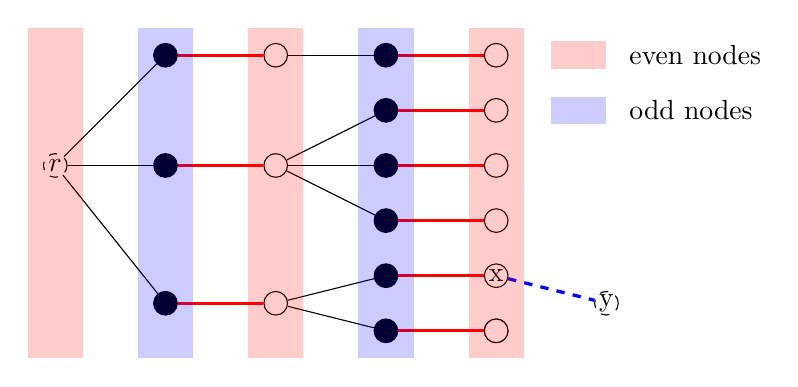
\begin{tikzpicture}[scale=0.7]
		\tikzstyle{Vertex} 	= [circle, draw, solid, fill=white, minimum size=3mm, inner sep=0pt]
		\tikzstyle{Exposed}	= [dashed]
		\tikzstyle{odd}	= [black]
		\tikzstyle{MC}		= [very thick, red]
		\tikzstyle{NM}		= [black]
			
		\node (v1) at (0, 0) [Vertex][Exposed] {$r$};
		\node (v2) at (2, 2) [Vertex][odd]{};
		\node (v3) at (2, 0) [Vertex][odd]{};
		\node (v4) at (2, -2.5) [Vertex][odd]{};
		\node (v5) at (4, 2) [Vertex]{};
		\node (v6) at (4, 0) [Vertex]{};
		\node (v7) at (4, -2.5) [Vertex]{};
		\node (v8) at (6, 2) [Vertex][odd]{};
		\node (v9) at (6, 1) [Vertex][odd]{};
		\node (v10) at (6, 0) [Vertex][odd]{};
		\node (v11) at (6, -1) [Vertex][odd]{};
		\node (v12) at (6, -2) [Vertex][odd]{};
		\node (v13) at (6, -3) [Vertex][odd]{};
		\node (v14) at (8, 2) [Vertex]{};
		\node (v15) at (8, 1) [Vertex]{};
		\node (v16) at (8, 0) [Vertex]{};
		\node (v17) at (8, -1) [Vertex]{};
		\node (v18) at (8, -2) [Vertex]{x};
		\node (v19) at (8, -3) [Vertex]{};
		\node (v19) at (8, -3) [Vertex]{};
		\node (v20) at (10, -2.5) [Vertex][Exposed]{y};
		
		\draw [-] (v1) to (v2) [NM];
		\draw [-] (v1) to (v3) [NM];
		\draw [-] (v1) to (v4) [NM];
		\draw [-] (v2) to (v5) [MC];
		\draw [-] (v3) to (v6) [MC];
		\draw [-] (v4) to (v7) [MC];
		\draw [-] (v5) to (v8) [NM];
		\draw [-] (v6) to (v9) [NM];
		\draw [-] (v6) to (v10) [NM];
		\draw [-] (v6) to (v11) [NM];
		\draw [-] (v7) to (v12) [NM];
		\draw [-] (v7) to (v13) [NM];
		\draw [-] (v8) to (v14) [MC];
		\draw [-] (v9) to (v15) [MC];
		\draw [-] (v10) to (v16) [MC];
		\draw [-] (v11) to (v17) [MC];
		\draw [-] (v12) to (v18) [MC];
		\draw [-] (v13) to (v19) [MC];
		\draw [-] (v18) to (v20) [dashed, blue, very thick];
		
		\fill[red, opacity = 0.2] (-0.5, 2.5) rectangle (0.5, -3.5);
		\fill[blue, opacity = 0.2] (2-0.5, 2.5) rectangle (2+0.5, -3.5);
		\fill[red, opacity = 0.2] (4-0.5, 2.5) rectangle (4+0.5, -3.5);
		\fill[blue, opacity = 0.2] (6-0.5, 2.5) rectangle (6+0.5, -3.5);
		\fill[red, opacity = 0.2] (8-0.5, 2.5) rectangle (8+0.5, -3.5);
		
		\draw (9,2) -- (10,2) [line width=10pt, red, opacity=0.2] node [right, black, opacity=1]{even nodes};
		\draw (9,1) -- (10,1) [line width=10pt, blue, opacity=0.2] node [right, black, opacity=1]{odd nodes};
	\end{tikzpicture}
	\end{center}
}

%---------------------slide--------------------%
\frame
{
	\frametitle{Find an augmenting path using BFS}
	
	\begin{overlayarea}{\textwidth}{1.5cm}
	Case 2, $y$ is matched vertex not in $T$, \alert{grow the tree}.
	\end{overlayarea}
		
	\begin{center}
	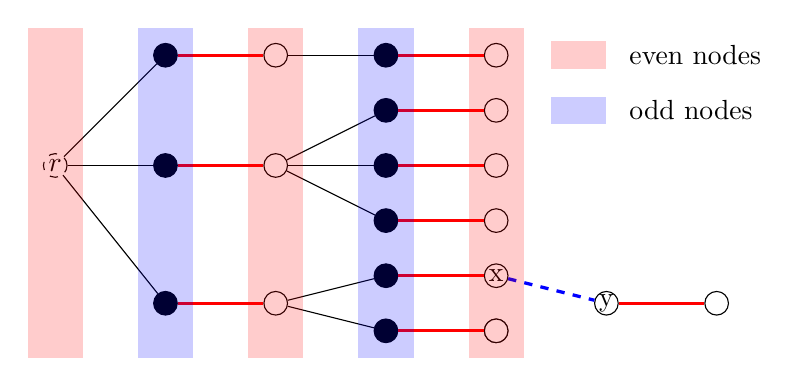
\begin{tikzpicture}[scale=0.7]
		\tikzstyle{Vertex} 	= [circle, draw, solid, fill=white, minimum size=3mm, inner sep=0pt]
		\tikzstyle{Exposed}	= [dashed]
		\tikzstyle{odd}	= [black]
		\tikzstyle{MC}		= [very thick, red]
		\tikzstyle{NM}		= [black]
			
		\node (v1) at (0, 0) [Vertex][Exposed] {$r$};
		\node (v2) at (2, 2) [Vertex][odd]{};
		\node (v3) at (2, 0) [Vertex][odd]{};
		\node (v4) at (2, -2.5) [Vertex][odd]{};
		\node (v5) at (4, 2) [Vertex]{};
		\node (v6) at (4, 0) [Vertex]{};
		\node (v7) at (4, -2.5) [Vertex]{};
		\node (v8) at (6, 2) [Vertex][odd]{};
		\node (v9) at (6, 1) [Vertex][odd]{};
		\node (v10) at (6, 0) [Vertex][odd]{};
		\node (v11) at (6, -1) [Vertex][odd]{};
		\node (v12) at (6, -2) [Vertex][odd]{};
		\node (v13) at (6, -3) [Vertex][odd]{};
		\node (v14) at (8, 2) [Vertex]{};
		\node (v15) at (8, 1) [Vertex]{};
		\node (v16) at (8, 0) [Vertex]{};
		\node (v17) at (8, -1) [Vertex]{};
		\node (v18) at (8, -2) [Vertex]{x};
		\node (v19) at (8, -3) [Vertex]{};
		\node (v19) at (8, -3) [Vertex]{};
		\node (v20) at (10, -2.5) [Vertex]{y};
		\node (v21) at (12, -2.5) [Vertex]{};
		
		\draw [-] (v1) to (v2) [NM];
		\draw [-] (v1) to (v3) [NM];
		\draw [-] (v1) to (v4) [NM];
		\draw [-] (v2) to (v5) [MC];
		\draw [-] (v3) to (v6) [MC];
		\draw [-] (v4) to (v7) [MC];
		\draw [-] (v5) to (v8) [NM];
		\draw [-] (v6) to (v9) [NM];
		\draw [-] (v6) to (v10) [NM];
		\draw [-] (v6) to (v11) [NM];
		\draw [-] (v7) to (v12) [NM];
		\draw [-] (v7) to (v13) [NM];
		\draw [-] (v8) to (v14) [MC];
		\draw [-] (v9) to (v15) [MC];
		\draw [-] (v10) to (v16) [MC];
		\draw [-] (v11) to (v17) [MC];
		\draw [-] (v12) to (v18) [MC];
		\draw [-] (v13) to (v19) [MC];
		\draw [-] (v18) to (v20) [dashed, blue, very thick];
		\draw [-] (v20) to (v21) [MC];
		
		\fill[red, opacity = 0.2] (-0.5, 2.5) rectangle (0.5, -3.5);
		\fill[blue, opacity = 0.2] (2-0.5, 2.5) rectangle (2+0.5, -3.5);
		\fill[red, opacity = 0.2] (4-0.5, 2.5) rectangle (4+0.5, -3.5);
		\fill[blue, opacity = 0.2] (6-0.5, 2.5) rectangle (6+0.5, -3.5);
		\fill[red, opacity = 0.2] (8-0.5, 2.5) rectangle (8+0.5, -3.5);
		
		\draw (9,2) -- (10,2) [line width=10pt, red, opacity=0.2] node [right, black, opacity=1]{even nodes};
		\draw (9,1) -- (10,1) [line width=10pt, blue, opacity=0.2] node [right, black, opacity=1]{odd nodes};
	\end{tikzpicture}
	\end{center}
}

%---------------------slide--------------------%
\frame
{
	\frametitle{Find an augmenting path using BFS}
	
	\begin{overlayarea}{\textwidth}{1.5cm}
	Case 3, $y$ is already contained in $T$ as an odd vertex. 
	
	\alert{Ignore it, no worry! Why?}
	\end{overlayarea}
		
	\begin{center}
	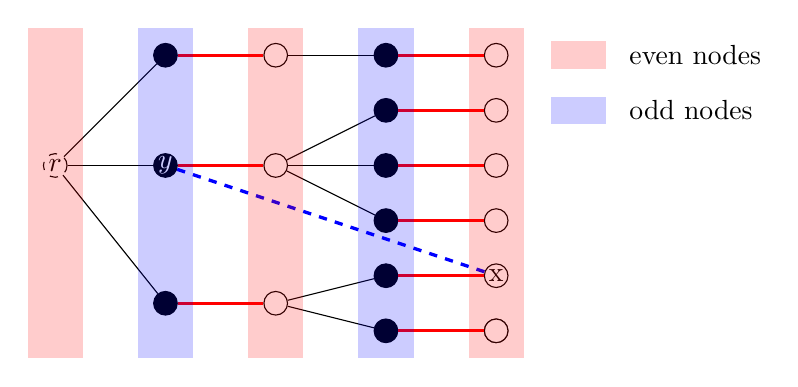
\begin{tikzpicture}[scale=0.7]
		\tikzstyle{Vertex} 	= [circle, draw, solid, fill=white, minimum size=3mm, inner sep=0pt]
		\tikzstyle{Exposed}	= [dashed]
		\tikzstyle{odd}	= [black]
		\tikzstyle{MC}		= [very thick, red]
		\tikzstyle{NM}		= [black]
			
		\node (v1) at (0, 0) [Vertex][Exposed] {$r$};
		\node (v2) at (2, 2) [Vertex][odd]{};
		\node (v3) at (2, 0) [Vertex][odd]{$\color{white}y$};
		\node (v4) at (2, -2.5) [Vertex][odd]{};
		\node (v5) at (4, 2) [Vertex]{};
		\node (v6) at (4, 0) [Vertex]{};
		\node (v7) at (4, -2.5) [Vertex]{};
		\node (v8) at (6, 2) [Vertex][odd]{};
		\node (v9) at (6, 1) [Vertex][odd]{};
		\node (v10) at (6, 0) [Vertex][odd]{};
		\node (v11) at (6, -1) [Vertex][odd]{};
		\node (v12) at (6, -2) [Vertex][odd]{};
		\node (v13) at (6, -3) [Vertex][odd]{};
		\node (v14) at (8, 2) [Vertex]{};
		\node (v15) at (8, 1) [Vertex]{};
		\node (v16) at (8, 0) [Vertex]{};
		\node (v17) at (8, -1) [Vertex]{};
		\node (v18) at (8, -2) [Vertex]{x};
		\node (v19) at (8, -3) [Vertex]{};
		\node (v19) at (8, -3) [Vertex]{};
		
		\draw [-] (v1) to (v2) [NM];
		\draw [-] (v1) to (v3) [NM];
		\draw [-] (v1) to (v4) [NM];
		\draw [-] (v2) to (v5) [MC];
		\draw [-] (v3) to (v6) [MC];
		\draw [-] (v4) to (v7) [MC];
		\draw [-] (v5) to (v8) [NM];
		\draw [-] (v6) to (v9) [NM];
		\draw [-] (v6) to (v10) [NM];
		\draw [-] (v6) to (v11) [NM];
		\draw [-] (v7) to (v12) [NM];
		\draw [-] (v7) to (v13) [NM];
		\draw [-] (v8) to (v14) [MC];
		\draw [-] (v9) to (v15) [MC];
		\draw [-] (v10) to (v16) [MC];
		\draw [-] (v11) to (v17) [MC];
		\draw [-] (v12) to (v18) [MC];
		\draw [-] (v13) to (v19) [MC];
		\draw [-] (v3) to (v18) [dashed, blue, very thick];
				
		\fill[red, opacity = 0.2] (-0.5, 2.5) rectangle (0.5, -3.5);
		\fill[blue, opacity = 0.2] (2-0.5, 2.5) rectangle (2+0.5, -3.5);
		\fill[red, opacity = 0.2] (4-0.5, 2.5) rectangle (4+0.5, -3.5);
		\fill[blue, opacity = 0.2] (6-0.5, 2.5) rectangle (6+0.5, -3.5);
		\fill[red, opacity = 0.2] (8-0.5, 2.5) rectangle (8+0.5, -3.5);
		
		\draw (9,2) -- (10,2) [line width=10pt, red, opacity=0.2] node [right, black, opacity=1]{even nodes};
		\draw (9,1) -- (10,1) [line width=10pt, blue, opacity=0.2] node [right, black, opacity=1]{odd nodes};
	\end{tikzpicture}
	\end{center}
}

%---------------------slide--------------------%
\frame
{
	\frametitle{Find an augmenting path using BFS}
	
	\begin{overlayarea}{\textwidth}{1.5cm}
	Case 4, $y$ is already contained in $T$ as an even vertex. 
	
	\alert{Can't ignore $y$, but it doesn't happen on a bipartite graph (no odd cycle)!}
	\end{overlayarea}
		
	\begin{center}
	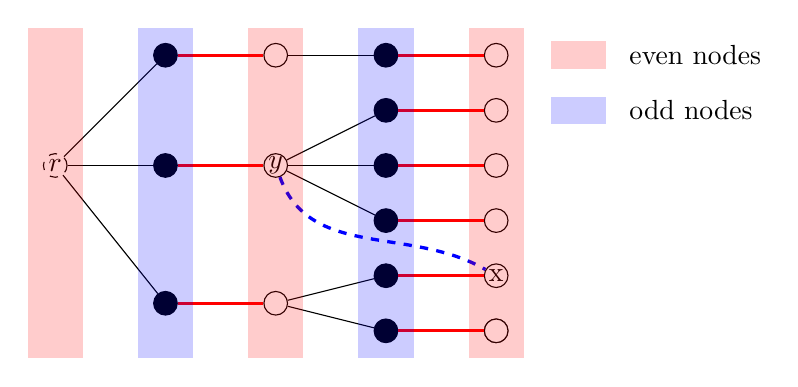
\begin{tikzpicture}[scale=0.7]
		\tikzstyle{Vertex} 	= [circle, draw, solid, fill=white, minimum size=3mm, inner sep=0pt]
		\tikzstyle{Exposed}	= [dashed]
		\tikzstyle{odd}	= [black]
		\tikzstyle{MC}		= [very thick, red]
		\tikzstyle{NM}		= [black]
			
		\node (v1) at (0, 0) [Vertex][Exposed] {$r$};
		\node (v2) at (2, 2) [Vertex][odd]{};
		\node (v3) at (2, 0) [Vertex][odd]{};
		\node (v4) at (2, -2.5) [Vertex][odd]{};
		\node (v5) at (4, 2) [Vertex]{};
		\node (v6) at (4, 0) [Vertex]{$y$};
		\node (v7) at (4, -2.5) [Vertex]{};
		\node (v8) at (6, 2) [Vertex][odd]{};
		\node (v9) at (6, 1) [Vertex][odd]{};
		\node (v10) at (6, 0) [Vertex][odd]{};
		\node (v11) at (6, -1) [Vertex][odd]{};
		\node (v12) at (6, -2) [Vertex][odd]{};
		\node (v13) at (6, -3) [Vertex][odd]{};
		\node (v14) at (8, 2) [Vertex]{};
		\node (v15) at (8, 1) [Vertex]{};
		\node (v16) at (8, 0) [Vertex]{};
		\node (v17) at (8, -1) [Vertex]{};
		\node (v18) at (8, -2) [Vertex]{x};
		\node (v19) at (8, -3) [Vertex]{};
		\node (v19) at (8, -3) [Vertex]{};
		
		\draw [-] (v1) to (v2) [NM];
		\draw [-] (v1) to (v3) [NM];
		\draw [-] (v1) to (v4) [NM];
		\draw [-] (v2) to (v5) [MC];
		\draw [-] (v3) to (v6) [MC];
		\draw [-] (v4) to (v7) [MC];
		\draw [-] (v5) to (v8) [NM];
		\draw [-] (v6) to (v9) [NM];
		\draw [-] (v6) to (v10) [NM];
		\draw [-] (v6) to (v11) [NM];
		\draw [-] (v7) to (v12) [NM];
		\draw [-] (v7) to (v13) [NM];
		\draw [-] (v8) to (v14) [MC];
		\draw [-] (v9) to (v15) [MC];
		\draw [-] (v10) to (v16) [MC];
		\draw [-] (v11) to (v17) [MC];
		\draw [-] (v12) to (v18) [MC];
		\draw [-] (v13) to (v19) [MC];
		\draw [-] (v6) to[in=150, out=-70] (v18) [dashed, blue, very thick];
				
		\fill[red, opacity = 0.2] (-0.5, 2.5) rectangle (0.5, -3.5);
		\fill[blue, opacity = 0.2] (2-0.5, 2.5) rectangle (2+0.5, -3.5);
		\fill[red, opacity = 0.2] (4-0.5, 2.5) rectangle (4+0.5, -3.5);
		\fill[blue, opacity = 0.2] (6-0.5, 2.5) rectangle (6+0.5, -3.5);
		\fill[red, opacity = 0.2] (8-0.5, 2.5) rectangle (8+0.5, -3.5);
		
		\draw (9,2) -- (10,2) [line width=10pt, red, opacity=0.2] node [right, black, opacity=1]{even nodes};
		\draw (9,1) -- (10,1) [line width=10pt, blue, opacity=0.2] node [right, black, opacity=1]{odd nodes};
	\end{tikzpicture}
	\end{center}
}

%%---------------------slide--------------------%
%\frame
%{
%	\frametitle{Find an augmenting path on bipartite graph}
%
%	\begin{center}
%	\begin{figure}[h]
%	\hfill
%		\centering
%		\begin{minipage}[c]{.45\textwidth}
%		\begin{tikzpicture}
%			\tikzstyle{Vertex} 	= [draw, solid,  fill=white, minimum size=6mm, inner sep=0pt]
%			\tikzstyle{Exposed}	= [dashed]
%			\tikzstyle{Boy}		= [circle]
%			\tikzstyle{Girl}	= [diamond, minimum size=7mm]
%			\tikzstyle{MC}		= [very thick, red]
%			\tikzstyle{NM}		= [gray]
%			
%			\node (b1) at (0,6) [Vertex][Boy][Exposed] {$1$};
%			\node (b2) at (0,5) [Vertex][Boy][Exposed] {$2$};
%			\node (b3) at (0,4) [Vertex][Boy] {$3$};
%			\node (b4) at (0,3) [Vertex][Boy] {$4$};
%			
%			\node (ga) at (4,6.00) [Vertex][Girl][Exposed] {$A$};
%			\node (gb) at (4,4.50) [Vertex][Girl] {$B$};
%			\node (gc) at (4,3.00) [Vertex][Girl] {$C$};
%			
%			\draw [-] (b1) to (gb) [NM];
%			\draw [-] (b2) to (gc) [NM];
%			\draw [-] (b3) to (gb) [NM];
%			\draw [-] (b3) to (gc) [MC];
%			\draw [-] (b4) to (ga) [NM];
%			\draw [-] (b4) to (gb) [MC];
%		\end{tikzpicture}
%		\end{minipage}
%	\hfill
%		\centering
%		\begin{minipage}[c]{.45\textwidth}
%			\begin{tikzpicture}
%				\tikzstyle{Vertex} 	= [draw, solid,  fill=white, minimum size=6mm, inner sep=0pt]
%				\tikzstyle{Exposed}	= [dashed]
%				\tikzstyle{Boy}		= [circle]
%				\tikzstyle{Girl}		= [diamond, minimum size=7mm]
%				\tikzstyle{MC}		= [very thick, red]
%				\tikzstyle{NM}		= [gray]
%				
%				\node (b1) at (0.0, 3) [Vertex][Boy][Exposed] {$1$};
%					
%				\node (gb) at (1.5, 3) [Vertex][Girl] {$B$};
%				
%				\node (b4) at (3.0, 3) [Vertex][Boy] {$4$};
%					
%				\node (ga) at (4.5, 3) [Vertex][Girl][Exposed] {$A$};
%				
%				\draw (b1) -- (gb) -- (b4) -- (ga) [line width=10pt, red, opacity=0.3];
%					
%				\draw [-] (b1) to (gb) [NM];
%				\draw [-] (b4) to (ga) [NM];
%				\draw [-] (b4) to (gb) [MC];
%			\end{tikzpicture}
%		\end{minipage}
%	\hfill
%	\end{figure}
%	\end{center}
%}

%%---------------------slide--------------------%
%\frame
%{
%	\frametitle{Find An Augmenting Path Using BFS}
%
%	\begin{center}
%	\begin{figure}[h]
%	\hfill
%		\centering
%		\begin{minipage}[c]{.45\textwidth}
%			\begin{tikzpicture}
%				\tikzstyle{Vertex} 	= [draw, solid,  fill=white, minimum size=6mm, inner sep=0pt]
%				\tikzstyle{Exposed}	= [dashed]
%				\tikzstyle{Boy}		= [circle]
%				\tikzstyle{Girl}		= [diamond, minimum size=7mm]
%				\tikzstyle{MC}		= [very thick, red]
%				\tikzstyle{NM}		= [gray]
%				
%				\node (b1) at (0,6) [Vertex][Boy] {$1$};
%				\node (b2) at (0,5) [Vertex][Boy][Exposed] {$2$};
%				\node (b3) at (0,4) [Vertex][Boy] {$3$};
%				\node (b4) at (0,3) [Vertex][Boy] {$4$};
%				
%				\node (ga) at (4,6.00) [Vertex][Girl] {$A$};
%				\node (gb) at (4,4.50) [Vertex][Girl] {$B$};
%				\node (gc) at (4,3.00) [Vertex][Girl] {$C$};
%				
%				\draw [-] (b1) to (gb) [MC];
%				\draw [-] (b2) to (gc) [NM];
%				\draw [-] (b3) to (gb) [NM];
%				\draw [-] (b3) to (gc) [MC];
%				\draw [-] (b4) to (ga) [MC];
%				\draw [-] (b4) to (gb) [NM];
%			\end{tikzpicture}
%		\end{minipage}
%	\hfill
%		\centering
%		\begin{minipage}[c]{.45\textwidth}
%			\begin{tikzpicture}
%				\tikzstyle{Vertex} 	= [draw, solid,  fill=white, minimum size=6mm, inner sep=0pt]
%				\tikzstyle{Exposed}	= [dashed]
%				\tikzstyle{Boy}		= [circle]
%				\tikzstyle{Girl}		= [diamond, minimum size=7mm]
%				\tikzstyle{MC}		= [very thick, red]
%				\tikzstyle{NM}		= [gray]
%				
%				\node (b2) at (0.0, 3) [Vertex][Boy][Exposed] {$2$};
%					
%				\node (gb) at (3, 3) [Vertex][Girl] {$B$};
%				\node (gc) at (1.0, 3) [Vertex][Girl] {$C$};
%				
%				\node (b1) at (4.0, 3) [Vertex][Boy] {$1$};
%				\node (b3) at (2.0, 3) [Vertex][Boy] {$3$};
%														
%				\draw [-] (b2) to (gc) [NM];
%				\draw [-] (b3) to (gb) [NM];
%				\draw [-] (b3) to (gc) [MC];
%				\draw [-] (b1) to (gb) [MC];
%			\end{tikzpicture}
%		\end{minipage}
%	\hfill
%	\end{figure}
%	\end{center}
%}

%---------------------slide--------------------%
\frame
{
	\frametitle{Summary}
	
	\uncover<1->{
	The algorithm grows an alternating tree from an exposed vertex, if we find an exposed vertex, we can enlarge the matching and start from another exposed vertex growing the tree again. 
	}
	
	\bigskip

	\uncover<2->{	
	After growing trees from all the exposed vertices, the algorithm terminates.
	}
	
	\bigskip

	\uncover<3->{	
	Time complexity $O(nm)$, $n$ is the number of vertices, $m$ is the number of edges.
	}
}

%---------------------slide--------------------%
\frame
{
	\frametitle{Question}
	\huge{Why will odd cycles be a trouble?}
}

%---------------------slide--------------------%
\frame
{
	\frametitle{Examples of BFS failure on non-bipartite graphs}
	\begin{overlayarea}{\textwidth}{1cm}
	\begin{itemize}
		\item Initial graph
	\end{itemize}
	\end{overlayarea}
	
	{\mode<presentation>{\tiny}
	\begin{center}
	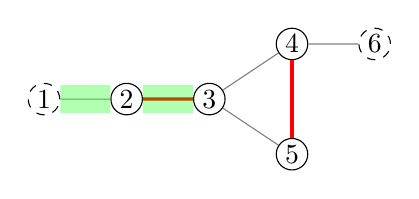
\begin{tikzpicture}[scale=0.7]
		\tikzstyle{Vertex} 	= [circle, draw, solid,  fill=white, minimum size=4mm, inner sep=0pt]
		\tikzstyle{Exposed}	= [dashed]
		\tikzstyle{MC}		= [very thick, red]
		\tikzstyle{NM}		= [gray]
			
		\node (v1) at (0.0, 5) [Vertex][Exposed] {$1$};
		\node (v2) at (1.5, 5) [Vertex] {$2$};
		\node (v3) at (3.0, 5) [Vertex] {$3$};
		\node (v4) at (4.5, 6) [Vertex] {$4$};
		\node (v5) at (4.5, 4) [Vertex] {$5$};
		\node (v6) at (6.0, 6) [Vertex][Exposed] {$6$};
			
		\draw [-] (v1) to (v2) [NM];
		\draw [-] (v2) to (v3) [MC];
		\draw [-] (v3) to (v4) [NM];
		\draw [-] (v3) to (v5) [NM];
		\draw [-] (v4) to (v5) [MC];
		\draw [-] (v4) to (v6) [NM];
		
		\draw (v1) -- (v2) -- (v3)[line width=10pt, green, opacity=0.3];
	\end{tikzpicture}
	\end{center}
	}

	\begin{overlayarea}{\textwidth}{1.5cm}
	\begin{itemize}
		\item Start from vertex 1, we add vertex 2 and 3.
	\end{itemize}
	\end{overlayarea}
	
	{\mode<presentation>{\tiny}
	\begin{center}
		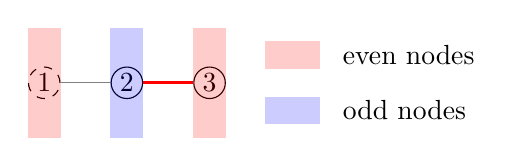
\begin{tikzpicture}[scale=0.7]
			\tikzstyle{Vertex} 	= [circle, draw, solid,  fill=white, minimum size=4mm, inner sep=0pt]
			\tikzstyle{Exposed}	= [dashed]
			\tikzstyle{MC}		= [very thick, red]
			\tikzstyle{NM}		= [gray]
			
			\node (v1) at (0.0, 0) [Vertex][Exposed] {$1$};
			\node (v2) at (1.5, 0) [Vertex] {$2$};
			\node (v3) at (3.0, 0) [Vertex] {$3$};
			
			\draw [-] (v1) to (v2) [NM];	
			\draw [-] (v2) to (v3) [MC];
			
			\fill[red, opacity = 0.2] (-0.3, 1) rectangle (0.3, -1);
			\fill[blue, opacity = 0.2] (1.5-0.3, 1) rectangle (1.5+0.3, -1);
			\fill[red, opacity = 0.2] (3-0.3, 1) rectangle (3+0.3, -1);
			
			\draw (4,0.5) -- (5,0.5) [line width=10pt, red, opacity=0.2] node [right, black, opacity=1]{even nodes};
			\draw (4,-0.5) -- (5,-0.5) [line width=10pt, blue, opacity=0.2] node [right, black, opacity=1]{odd nodes};
		\end{tikzpicture}
	\end{center}
	}
}

%---------------------slide--------------------%
\frame
{
	\frametitle{Examples of BFS failure on non-bipartite graphs}
	
	\begin{overlayarea}{\textwidth}{1cm}
	\begin{itemize}
		\item Initial graph
	\end{itemize}
	\end{overlayarea}
	
	{\mode<presentation>{\tiny}
	\begin{center}
	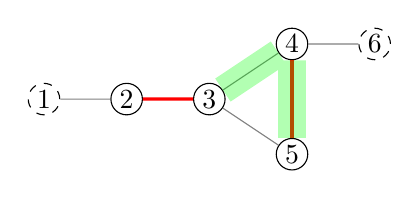
\begin{tikzpicture}[scale=0.7]
		\tikzstyle{Vertex} 	= [circle, draw, solid,  fill=white, minimum size=4mm, inner sep=0pt]
		\tikzstyle{Exposed}	= [dashed]
		\tikzstyle{MC}		= [very thick, red]
		\tikzstyle{NM}		= [gray]
			
		\node (v1) at (0.0, 5) [Vertex][Exposed] {$1$};
		\node (v2) at (1.5, 5) [Vertex] {$2$};
		\node (v3) at (3.0, 5) [Vertex] {$3$};
		\node (v4) at (4.5, 6) [Vertex] {$4$};
		\node (v5) at (4.5, 4) [Vertex] {$5$};
		\node (v6) at (6.0, 6) [Vertex][Exposed] {$6$};
			
		\draw [-] (v1) to (v2) [NM];	
		\draw [-] (v2) to (v3) [MC];
		\draw [-] (v3) to (v4) [NM];
		\draw [-] (v3) to (v5) [NM];
		\draw [-] (v4) to (v5) [MC];
		\draw [-] (v4) to (v6) [NM];
		
		\draw (v3) -- (v4) -- (v5)[line width=10pt, green, opacity=0.3];
	\end{tikzpicture}
	\end{center}
	}

	\begin{overlayarea}{\textwidth}{1.5cm}
	\begin{itemize}
		\item Two vertices 4 and 5 could be visited. If we first visit 4...
	\end{itemize}
	\end{overlayarea}
	
	{\mode<presentation>{\tiny}
	\begin{center}
		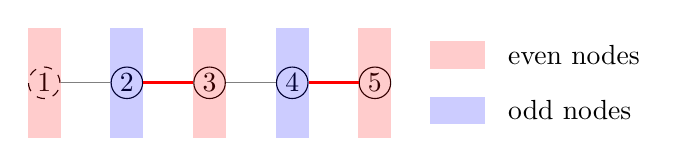
\begin{tikzpicture}[scale=0.7]
			\tikzstyle{Vertex} 	= [circle, draw, solid,  fill=white, minimum size=4mm, inner sep=0pt]
			\tikzstyle{Exposed}	= [dashed]
			\tikzstyle{MC}		= [very thick, red]
			\tikzstyle{NM}		= [gray]
			
			\node (v1) at (0.0, 0) [Vertex][Exposed] {$1$};
			\node (v2) at (1.5, 0) [Vertex] {$2$};
			\node (v3) at (3.0, 0) [Vertex] {$3$};
			\node (v4) at (4.5, 0) [Vertex] {$4$};
			\node (v5) at (6.0, 0) [Vertex] {$5$};
			
			\draw [-] (v1) to (v2) [NM];	
			\draw [-] (v2) to (v3) [MC];
			\draw [-] (v3) to (v4) [NM];
			\draw [-] (v4) to (v5) [MC];
			
			\fill[red, opacity = 0.2] (-0.3, 1) rectangle (0.3, -1);
			\fill[blue, opacity = 0.2] (1.5-0.3, 1) rectangle (1.5+0.3, -1);
			\fill[red, opacity = 0.2] (3-0.3, 1) rectangle (3+0.3, -1);
			\fill[blue, opacity = 0.2] (4.5-0.3, 1) rectangle (4.5+0.3, -1);
			\fill[red, opacity = 0.2] (6-0.3, 1) rectangle (6+0.3, -1);
			
			\draw (7,0.5) -- (8,0.5) [line width=10pt, red, opacity=0.2] node [right, black, opacity=1]{even nodes};
			\draw (7,-0.5) -- (8,-0.5) [line width=10pt, blue, opacity=0.2] node [right, black, opacity=1]{odd nodes};
		\end{tikzpicture}
	\end{center}
	}
}

%---------------------slide--------------------%
\frame
{
	\frametitle{Examples of BFS failure on non-bipartite graphs}
	
	\begin{overlayarea}{\textwidth}{1cm}
	\begin{itemize}
		\item Initial graph
	\end{itemize}
	\end{overlayarea}
	
	{\mode<presentation>{\tiny}
	\begin{center}
	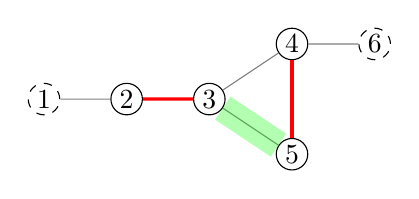
\begin{tikzpicture}[scale=0.7]
		\tikzstyle{Vertex} 	= [circle, draw, solid,  fill=white, minimum size=4mm, inner sep=0pt]
		\tikzstyle{Exposed}	= [dashed]
		\tikzstyle{MC}		= [very thick, red]
		\tikzstyle{NM}		= [gray]
			
		\node (v1) at (0.0, 5) [Vertex][Exposed] {$1$};
		\node (v2) at (1.5, 5) [Vertex] {$2$};
		\node (v3) at (3.0, 5) [Vertex] {$3$};
		\node (v4) at (4.5, 6) [Vertex] {$4$};
		\node (v5) at (4.5, 4) [Vertex] {$5$};
		\node (v6) at (6.0, 6) [Vertex][Exposed] {$6$};
			
		\draw [-] (v1) to (v2) [NM];	
		\draw [-] (v2) to (v3) [MC];
		\draw [-] (v3) to (v4) [NM];
		\draw [-] (v3) to (v5) [NM];
		\draw [-] (v4) to (v5) [MC];
		\draw [-] (v4) to (v6) [NM];	
		
		\draw (v3) -- (v5)[line width=10pt, green, opacity=0.3];
	\end{tikzpicture}
	\end{center}
	}

	\begin{overlayarea}{\textwidth}{1.5cm}
	\begin{itemize}
		\item From 5, we find 3 which is contained in $T$, if we ignore it, we will stop here.
	\end{itemize}
	\end{overlayarea}
	
	{\mode<presentation>{\tiny}
	\begin{center}
		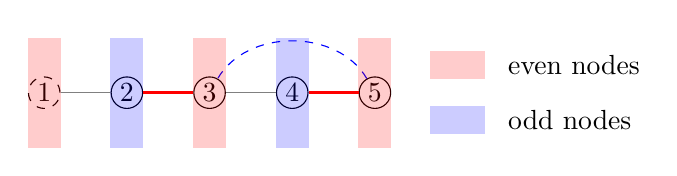
\begin{tikzpicture}[scale=0.7]
			\tikzstyle{Vertex} 	= [circle, draw, solid,  fill=white, minimum size=4mm, inner sep=0pt]
			\tikzstyle{Exposed}	= [dashed]
			\tikzstyle{MC}		= [very thick, red]
			\tikzstyle{NM}		= [gray]
			
			\node (v1) at (0.0, 0) [Vertex][Exposed] {$1$};
			\node (v2) at (1.5, 0) [Vertex] {$2$};
			\node (v3) at (3.0, 0) [Vertex] {$3$};
			\node (v4) at (4.5, 0) [Vertex] {$4$};
			\node (v5) at (6.0, 0) [Vertex] {$5$};
			
			\draw [-] (v1) to (v2) [NM];	
			\draw [-] (v2) to (v3) [MC];
			\draw [-] (v3) to (v4) [NM];
			\draw [-] (v4) to (v5) [MC];
			\draw [-] (v5) to[in=60, out=120] (v3) [dashed][blue];
			
			\fill[red, opacity = 0.2] (-0.3, 1) rectangle (0.3, -1);
			\fill[blue, opacity = 0.2] (1.5-0.3, 1) rectangle (1.5+0.3, -1);
			\fill[red, opacity = 0.2] (3-0.3, 1) rectangle (3+0.3, -1);
			\fill[blue, opacity = 0.2] (4.5-0.3, 1) rectangle (4.5+0.3, -1);
			\fill[red, opacity = 0.2] (6-0.3, 1) rectangle (6+0.3, -1);
			
			\draw (7,0.5) -- (8,0.5) [line width=10pt, red, opacity=0.2] node [right, black, opacity=1]{even nodes};
			\draw (7,-0.5) -- (8,-0.5) [line width=10pt, blue, opacity=0.2] node [right, black, opacity=1]{odd nodes};
		\end{tikzpicture}
	\end{center}
	}
}

%---------------------slide--------------------%
\frame
{
	\frametitle{Examples of BFS failure on non-bipartite graphs}
	
	\begin{overlayarea}{\textwidth}{1cm}
	\begin{itemize}
		\item Initial graph
	\end{itemize}
	\end{overlayarea}
	
	{\mode<presentation>{\tiny}
	\begin{center}
	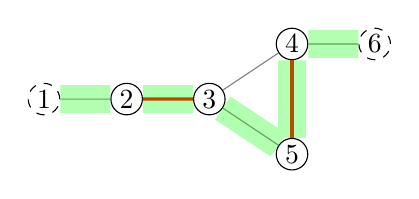
\begin{tikzpicture}[scale=0.7]
		\tikzstyle{Vertex} 	= [circle, draw, solid,  fill=white, minimum size=4mm, inner sep=0pt]
		\tikzstyle{Exposed}	= [dashed]
		\tikzstyle{MC}		= [very thick, red]
		\tikzstyle{NM}		= [gray]
			
		\node (v1) at (0.0, 5) [Vertex][Exposed] {$1$};
		\node (v2) at (1.5, 5) [Vertex] {$2$};
		\node (v3) at (3.0, 5) [Vertex] {$3$};
		\node (v4) at (4.5, 6) [Vertex] {$4$};
		\node (v5) at (4.5, 4) [Vertex] {$5$};
		\node (v6) at (6.0, 6) [Vertex][Exposed] {$6$};
			
		\draw [-] (v1) to (v2) [NM];	
		\draw [-] (v2) to (v3) [MC];
		\draw [-] (v3) to (v4) [NM];
		\draw [-] (v3) to (v5) [NM];
		\draw [-] (v4) to (v5) [MC];
		\draw [-] (v4) to (v6) [NM];
		
		\draw (v1) -- (v2) -- (v3) -- (v5) -- (v4) -- (v6)[line width=10pt, green, opacity=0.3];	
	\end{tikzpicture}
	\end{center}
	}

	\begin{overlayarea}{\textwidth}{1.5cm}
	\begin{itemize}
		\item But actually there is an augmenting path!
	\end{itemize}
	\end{overlayarea}
	
	{\mode<presentation>{\tiny}
	\begin{center}
		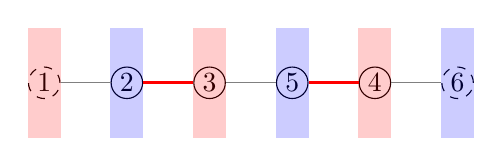
\begin{tikzpicture}[scale=0.7]
			\tikzstyle{Vertex} 	= [circle, draw, solid,  fill=white, minimum size=4mm, inner sep=0pt]
			\tikzstyle{Exposed}	= [dashed]
			\tikzstyle{MC}		= [very thick, red]
			\tikzstyle{NM}		= [gray]
				
			\node (v1) at (0.0, 0) [Vertex][Exposed] {$1$};
			\node (v2) at (1.5, 0) [Vertex] {$2$};
			\node (v3) at (3.0, 0) [Vertex] {$3$};
			\node (v4) at (6.0, 0) [Vertex] {$4$};
			\node (v5) at (4.5, 0) [Vertex] {$5$};
			\node (v6) at (7.5, 0) [Vertex][Exposed] {$6$};
			
			\fill[red, opacity = 0.2] (-0.3, 1) rectangle (0.3, -1);
			\fill[blue, opacity = 0.2] (1.5-0.3, 1) rectangle (1.5+0.3, -1);
			\fill[red, opacity = 0.2] (3-0.3, 1) rectangle (3+0.3, -1);
			\fill[blue, opacity = 0.2] (4.5-0.3, 1) rectangle (4.5+0.3, -1);
			\fill[red, opacity = 0.2] (6-0.3, 1) rectangle (6+0.3, -1);
			\fill[blue, opacity = 0.2] (7.5-0.3, 1) rectangle (7.5+0.3, -1);
			
			\draw [-] (v1) to (v2) [NM];	
			\draw [-] (v2) to (v3) [MC];
			\draw [-] (v3) to (v5) [NM];
			\draw [-] (v5) to (v4) [MC];
			\draw [-] (v4) to (v6) [NM];
		\end{tikzpicture}
	\end{center}
	}
}

%---------------------slide--------------------%
\frame
{
	\frametitle{Examples of BFS failure on non-bipartite graphs}
	
	\begin{overlayarea}{\textwidth}{1cm}
	\begin{itemize}
		\item Initial graph
	\end{itemize}
	\end{overlayarea}
	
	{\mode<presentation>{\tiny}
	\begin{center}
	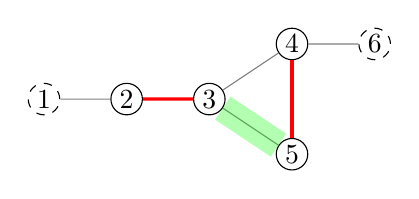
\begin{tikzpicture}[scale=0.7]
		\tikzstyle{Vertex} 	= [circle, draw, solid,  fill=white, minimum size=4mm, inner sep=0pt]
		\tikzstyle{Exposed}	= [dashed]
		\tikzstyle{MC}		= [very thick, red]
		\tikzstyle{NM}		= [gray]
			
		\node (v1) at (0.0, 5) [Vertex][Exposed] {$1$};
		\node (v2) at (1.5, 5) [Vertex] {$2$};
		\node (v3) at (3.0, 5) [Vertex] {$3$};
		\node (v4) at (4.5, 6) [Vertex] {$4$};
		\node (v5) at (4.5, 4) [Vertex] {$5$};
		\node (v6) at (6.0, 6) [Vertex][Exposed] {$6$};
			
		\draw [-] (v1) to (v2) [NM];	
		\draw [-] (v2) to (v3) [MC];
		\draw [-] (v3) to (v4) [NM];
		\draw [-] (v3) to (v5) [NM];
		\draw [-] (v4) to (v5) [MC];
		\draw [-] (v4) to (v6) [NM];	
		
		\draw (v3) -- (v5)[line width=10pt, green, opacity=0.3];
	\end{tikzpicture}
	\end{center}
	}

	\begin{overlayarea}{\textwidth}{1.5cm}
	\begin{itemize}
		\item The problem is that 3 already been visited in even layer, and 5 is also in even layer. But the tree must alternate between different layers.
	\end{itemize}
	\end{overlayarea}
	
	{\mode<presentation>{\tiny}
	\begin{center}
		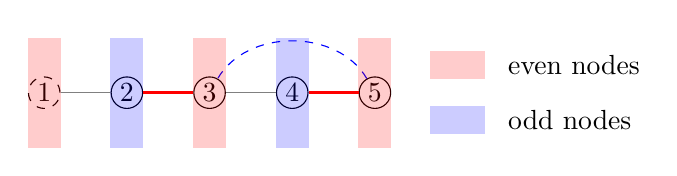
\begin{tikzpicture}[scale=0.7]
			\tikzstyle{Vertex} 	= [circle, draw, solid,  fill=white, minimum size=4mm, inner sep=0pt]
			\tikzstyle{Exposed}	= [dashed]
			\tikzstyle{MC}		= [very thick, red]
			\tikzstyle{NM}		= [gray]
			
			\node (v1) at (0.0, 0) [Vertex][Exposed] {$1$};
			\node (v2) at (1.5, 0) [Vertex] {$2$};
			\node (v3) at (3.0, 0) [Vertex] {$3$};
			\node (v4) at (4.5, 0) [Vertex] {$4$};
			\node (v5) at (6.0, 0) [Vertex] {$5$};
			
			\draw [-] (v1) to (v2) [NM];	
			\draw [-] (v2) to (v3) [MC];
			\draw [-] (v3) to (v4) [NM];
			\draw [-] (v4) to (v5) [MC];
			\draw [-] (v5) to[in=60, out=120] (v3) [dashed][blue];
			
			\fill[red, opacity = 0.2] (-0.3, 1) rectangle (0.3, -1);
			\fill[blue, opacity = 0.2] (1.5-0.3, 1) rectangle (1.5+0.3, -1);
			\fill[red, opacity = 0.2] (3-0.3, 1) rectangle (3+0.3, -1);
			\fill[blue, opacity = 0.2] (4.5-0.3, 1) rectangle (4.5+0.3, -1);
			\fill[red, opacity = 0.2] (6-0.3, 1) rectangle (6+0.3, -1);
			
			\draw (7,0.5) -- (8,0.5) [line width=10pt, red, opacity=0.2] node [right, black, opacity=1]{even nodes};
			\draw (7,-0.5) -- (8,-0.5) [line width=10pt, blue, opacity=0.2] node [right, black, opacity=1]{odd nodes};
		\end{tikzpicture}
	\end{center}
	}
}

%---------------------slide--------------------%
\frame
{
	\frametitle{Examples of BFS failure on non-bipartite graphs}
	
	\begin{overlayarea}{\textwidth}{1cm}
	\begin{itemize}
		\item Initial graph
	\end{itemize}
	\end{overlayarea}
	
	{\mode<presentation>{\tiny}
	\begin{center}
	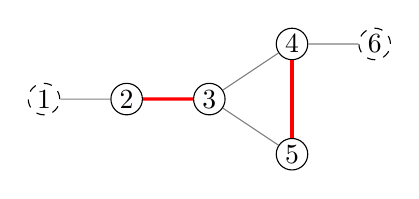
\begin{tikzpicture}[scale=0.7]
		\tikzstyle{Vertex} 	= [circle, draw, solid,  fill=white, minimum size=4mm, inner sep=0pt]
		\tikzstyle{Exposed}	= [dashed]
		\tikzstyle{MC}		= [very thick, red]
		\tikzstyle{NM}		= [gray]
			
		\node (v1) at (0.0, 5) [Vertex][Exposed] {$1$};
		\node (v2) at (1.5, 5) [Vertex] {$2$};
		\node (v3) at (3.0, 5) [Vertex] {$3$};
		\node (v4) at (4.5, 6) [Vertex] {$4$};
		\node (v5) at (4.5, 4) [Vertex] {$5$};
		\node (v6) at (6.0, 6) [Vertex][Exposed] {$6$};
			
		\draw [-] (v1) to (v2) [NM];	
		\draw [-] (v2) to (v3) [MC];
		\draw [-] (v3) to (v4) [NM];
		\draw [-] (v3) to (v5) [NM];
		\draw [-] (v4) to (v5) [MC];
		\draw [-] (v4) to (v6) [NM];	
		
	\end{tikzpicture}
	\end{center}
	}

	\begin{overlayarea}{\textwidth}{1.5cm}
	\begin{itemize}
		\item First idea: allow vertices to be visited both even and odd layers.
	\end{itemize}
	\end{overlayarea}
	
	{\mode<presentation>{\tiny}
	\begin{center}
		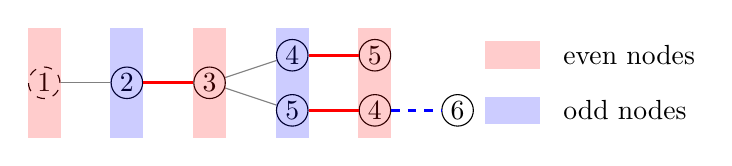
\begin{tikzpicture}[scale=0.7]
			\tikzstyle{Vertex} 	= [circle, draw, solid,  fill=white, minimum size=4mm, inner sep=0pt]
			\tikzstyle{Exposed}	= [dashed]
			\tikzstyle{MC}		= [very thick, red]
			\tikzstyle{NM}		= [gray]
			
			\node (v1) at (0.0, 0) [Vertex][Exposed] {$1$};
			\node (v2) at (1.5, 0) [Vertex] {$2$};
			\node (v3) at (3.0, 0) [Vertex] {$3$};
			\node (v4) at (4.5, 0.5) [Vertex] {$4$};
			\node (v5) at (6.0, 0.5) [Vertex] {$5$};
			\node (v6) at (4.5, -0.5) [Vertex] {$5$};
			\node (v7) at (6.0, -0.5) [Vertex] {$4$};
			\node (v8) at (7.5, -0.5) [Vertex] {$6$};
			
			\draw [-] (v1) to (v2) [NM];	
			\draw [-] (v2) to (v3) [MC];
			\draw [-] (v3) to (v4) [NM];
			\draw [-] (v4) to (v5) [MC];
			\draw [-] (v3) to (v6) [NM];
			\draw [-] (v6) to (v7) [MC];
			\draw [-] (v7) to (v8) [dashed, very thick][blue];
			
			\fill[red, opacity = 0.2] (-0.3, 1) rectangle (0.3, -1);
			\fill[blue, opacity = 0.2] (1.5-0.3, 1) rectangle (1.5+0.3, -1);
			\fill[red, opacity = 0.2] (3-0.3, 1) rectangle (3+0.3, -1);
			\fill[blue, opacity = 0.2] (4.5-0.3, 1) rectangle (4.5+0.3, -1);
			\fill[red, opacity = 0.2] (6-0.3, 1) rectangle (6+0.3, -1);
			
			\draw (8,0.5) -- (9,0.5) [line width=10pt, red, opacity=0.2] node [right, black, opacity=1]{even nodes};
			\draw (8,-0.5) -- (9,-0.5) [line width=10pt, blue, opacity=0.2] node [right, black, opacity=1]{odd nodes};
		\end{tikzpicture}
	\end{center}
	}
}

%---------------------slide--------------------%
\frame
{
	\frametitle{Examples of BFS failure on non-bipartite graphs}
	
	\begin{overlayarea}{\textwidth}{1cm}
	\begin{itemize}
		\item Initial graph
	\end{itemize}
	\end{overlayarea}
	
	{\mode<presentation>{\tiny}
	\begin{center}
	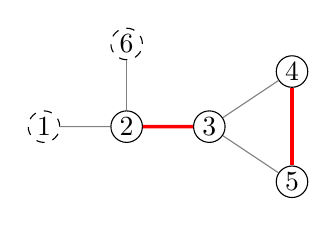
\begin{tikzpicture}[scale=0.7]
		\tikzstyle{Vertex} 	= [circle, draw, solid,  fill=white, minimum size=4mm, inner sep=0pt]
		\tikzstyle{Exposed}	= [dashed]
		\tikzstyle{MC}		= [very thick, red]
		\tikzstyle{NM}		= [gray]
			
		\node (v1) at (0.0, 5) [Vertex][Exposed] {$1$};
		\node (v2) at (1.5, 5) [Vertex] {$2$};
		\node (v3) at (3.0, 5) [Vertex] {$3$};
		\node (v4) at (4.5, 6) [Vertex] {$4$};
		\node (v5) at (4.5, 4) [Vertex] {$5$};
		\node (v6) at (1.5, 6.5) [Vertex][Exposed] {$6$};
			
		\draw [-] (v1) to (v2) [NM];	
		\draw [-] (v2) to (v3) [MC];
		\draw [-] (v3) to (v4) [NM];
		\draw [-] (v3) to (v5) [NM];
		\draw [-] (v4) to (v5) [MC];
		\draw [-] (v2) to (v6) [NM];	
	\end{tikzpicture}
	\end{center}
	}

	\begin{overlayarea}{\textwidth}{1.5cm}
	\begin{itemize}
		\item But the augmenting path we find may not be a simple path.
	\end{itemize}
	\end{overlayarea}
	
	{\mode<presentation>{\tiny}
	\begin{center}
		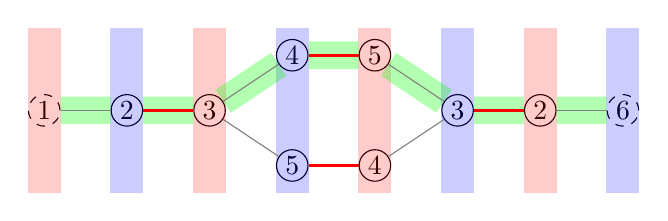
\begin{tikzpicture}[scale=0.7]
			\tikzstyle{Vertex} 	= [circle, draw, solid,  fill=white, minimum size=4mm, inner sep=0pt]
			\tikzstyle{Exposed}	= [dashed]
			\tikzstyle{MC}		= [very thick, red]
			\tikzstyle{NM}		= [gray]
				
			\node (v1) at (0.0, 0) [Vertex][Exposed] {$1$};
			\node (v2) at (1.5, 0) [Vertex] {$2$};
			\node (v22) at (9.0, 0) [Vertex] {$2$};
			\node (v3) at (3.0, 0) [Vertex] {$3$};
			\node (v32) at (7.5, 0) [Vertex] {$3$};
			\node (v4) at (4.5, 1) [Vertex] {$4$};
			\node (v42) at (6.0, -1) [Vertex] {$4$};
			\node (v5) at (6.0, 1) [Vertex] {$5$};
			\node (v52) at (4.5, -1) [Vertex] {$5$};
			\node (v6) at (10.5, 0) [Vertex][Exposed] {$6$};
			
			\fill[red, opacity = 0.2] (-0.3, 1.5) rectangle (0.3, -1.5);
			\fill[blue, opacity = 0.2] (1.5-0.3, 1.5) rectangle (1.5+0.3, -1.5);
			\fill[red, opacity = 0.2] (3-0.3, 1.5) rectangle (3+0.3, -1.5);
			\fill[blue, opacity = 0.2] (4.5-0.3, 1.5) rectangle (4.5+0.3, -1.5);
			\fill[red, opacity = 0.2] (6-0.3, 1.5) rectangle (6+0.3, -1.5);
			\fill[blue, opacity = 0.2] (7.5-0.3, 1.5) rectangle (7.5+0.3, -1.5);
			\fill[red, opacity = 0.2] (9-0.3, 1.5) rectangle (9+0.3, -1.5);
			\fill[blue, opacity = 0.2] (10.5-0.3, 1.5) rectangle (10.5+0.3, -1.5);
			
			\draw (v1) -- (v2) -- (v3) -- (v4) -- (v5) -- (v32) -- (v22) -- (v6)[line width=10pt, green, opacity=0.3];
			
			\draw [-] (v1) to (v2) [NM];	
			\draw [-] (v2) to (v3) [MC];
			\draw [-] (v3) to (v4) [NM];
			\draw [-] (v4) to (v5) [MC];
			\draw [-] (v5) to (v32) [NM];
			\draw [-] (v32) to (v22) [MC];
			\draw [-] (v22) to (v6) [NM];
			\draw [-] (v3) to (v52) [NM];
			\draw [-] (v52) to (v42) [MC];
			\draw [-] (v42) to (v32) [NM];
		\end{tikzpicture}
	\end{center}
	}
}

%---------------------slide--------------------%
\frame
{
	\frametitle{Examples of BFS failure on non-bipartite graphs}

	\begin{overlayarea}{\textwidth}{1cm}
	\begin{itemize}
	\item Result graph
	\end{itemize}
	\end{overlayarea}
	
	{\mode<presentation>{\tiny}
	\begin{center}
	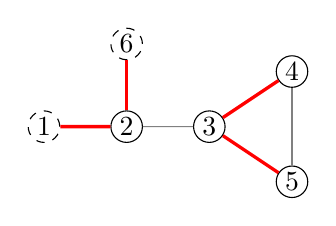
\begin{tikzpicture}[scale=0.7]
		\tikzstyle{Vertex} 	= [circle, draw, solid,  fill=white, minimum size=4mm, inner sep=0pt]
		\tikzstyle{Exposed}	= [dashed]
		\tikzstyle{MC}		= [very thick, red]
		\tikzstyle{NM}		= [gray]
			
		\node (v1) at (0.0, 5) [Vertex][Exposed] {$1$};
		\node (v2) at (1.5, 5) [Vertex] {$2$};
		\node (v3) at (3.0, 5) [Vertex] {$3$};
		\node (v4) at (4.5, 6) [Vertex] {$4$};
		\node (v5) at (4.5, 4) [Vertex] {$5$};
		\node (v6) at (1.5, 6.5) [Vertex][Exposed] {$6$};
			
		\draw [-] (v1) to (v2) [MC];	
		\draw [-] (v2) to (v3) [NM];
		\draw [-] (v3) to (v4) [MC];
		\draw [-] (v3) to (v5) [MC];
		\draw [-] (v4) to (v5) [NM];
		\draw [-] (v2) to (v6) [MC];	
	\end{tikzpicture}
	\end{center}
	}

	\begin{overlayarea}{\textwidth}{1.5cm}
	\begin{itemize}
		\item If we flip the edges...
	\end{itemize}
	\end{overlayarea}
	
	{\mode<presentation>{\tiny}
	\begin{center}
		\begin{tikzpicture}[scale=0.7]
			\tikzstyle{Vertex} 	= [circle, draw, solid,  fill=white, minimum size=4mm, inner sep=0pt]
			\tikzstyle{Exposed}	= [dashed]
			\tikzstyle{MC}		= [very thick, red]
			\tikzstyle{NM}		= [gray]
				
			\node (v1) at (0.0, 0) [Vertex][Exposed] {$1$};
			\node (v2) at (1.5, 0) [Vertex] {$2$};
			\node (v22) at (9.0, 0) [Vertex] {$2$};
			\node (v3) at (3.0, 0) [Vertex] {$3$};
			\node (v32) at (7.5, 0) [Vertex] {$3$};
			\node (v4) at (4.5, 1) [Vertex] {$4$};
			\node (v42) at (6.0, -1) [Vertex] {$4$};
			\node (v5) at (6.0, 1) [Vertex] {$5$};
			\node (v52) at (4.5, -1) [Vertex] {$5$};
			\node (v6) at (10.5, 0) [Vertex][Exposed] {$6$};
			
			\fill[red, opacity = 0.2] (-0.3, 1.5) rectangle (0.3, -1.5);
			\fill[blue, opacity = 0.2] (1.5-0.3, 1.5) rectangle (1.5+0.3, -1.5);
			\fill[red, opacity = 0.2] (3-0.3, 1.5) rectangle (3+0.3, -1.5);
			\fill[blue, opacity = 0.2] (4.5-0.3, 1.5) rectangle (4.5+0.3, -1.5);
			\fill[red, opacity = 0.2] (6-0.3, 1.5) rectangle (6+0.3, -1.5);
			\fill[blue, opacity = 0.2] (7.5-0.3, 1.5) rectangle (7.5+0.3, -1.5);
			\fill[red, opacity = 0.2] (9-0.3, 1.5) rectangle (9+0.3, -1.5);
			\fill[blue, opacity = 0.2] (10.5-0.3, 1.5) rectangle (10.5+0.3, -1.5);
			
			\draw (v1) -- (v2) -- (v3) -- (v4) -- (v5) -- (v32) -- (v22) -- (v6)[line width=10pt, green, opacity=0.3];
			
			\draw [-] (v1) to (v2) [MC];	
			\draw [-] (v2) to (v3) [NM];
			\draw [-] (v3) to (v4) [MC];
			\draw [-] (v4) to (v5) [NM];
			\draw [-] (v5) to (v32) [MC];
			\draw [-] (v32) to (v22) [NM];
			\draw [-] (v22) to (v6) [MC];
			\draw [-] (v3) to (v52) [NM];
			\draw [-] (v52) to (v42) [MC];
			\draw [-] (v42) to (v32) [NM];
		\end{tikzpicture}
	\end{center}
	}
}

%---------------------slide--------------------%
\frame
{
	\frametitle{Review}
	
	\begin{overlayarea}{\textwidth}{2cm}
	The frontier of the BFS consist of only even nodes, from where we extend the search tree.
	\end{overlayarea}
	
	\begin{center}
	\begin{tikzpicture}[scale=0.7]
		\tikzstyle{Vertex} 	= [circle, draw, solid, fill=white, minimum size=3mm, inner sep=0pt]
		\tikzstyle{Exposed}	= [dashed]
		\tikzstyle{odd}	= [black]
		\tikzstyle{MC}		= [very thick, red]
		\tikzstyle{NM}		= [black]
			
		\node (v1) at (0, 0) [Vertex][Exposed] {$r$};
		\node (v2) at (2, 2) [Vertex][odd]{};
		\node (v3) at (2, 0) [Vertex][odd]{};
		\node (v4) at (2, -2.5) [Vertex][odd]{};
		\node (v5) at (4, 2) [Vertex]{};
		\node (v6) at (4, 0) [Vertex]{};
		\node (v7) at (4, -2.5) [Vertex]{};
		\node (v8) at (6, 2) [Vertex][odd]{};
		\node (v9) at (6, 1) [Vertex][odd]{};
		\node (v10) at (6, 0) [Vertex][odd]{};
		\node (v11) at (6, -1) [Vertex][odd]{};
		\node (v12) at (6, -2) [Vertex][odd]{};
		\node (v13) at (6, -3) [Vertex][odd]{};
		\node (v14) at (8, 2) [Vertex]{};
		\node (v15) at (8, 1) [Vertex]{};
		\node (v16) at (8, 0) [Vertex]{};
		\node (v17) at (8, -1) [Vertex]{};
		\node (v18) at (8, -2) [Vertex]{};
		\node (v19) at (8, -3) [Vertex]{};
			
		\draw [-] (v1) to (v2) [NM];
		\draw [-] (v1) to (v3) [NM];
		\draw [-] (v1) to (v4) [NM];
		\draw [-] (v2) to (v5) [MC];
		\draw [-] (v3) to (v6) [MC];
		\draw [-] (v4) to (v7) [MC];
		\draw [-] (v5) to (v8) [NM];
		\draw [-] (v6) to (v9) [NM];
		\draw [-] (v6) to (v10) [NM];
		\draw [-] (v6) to (v11) [NM];
		\draw [-] (v7) to (v12) [NM];
		\draw [-] (v7) to (v13) [NM];
		\draw [-] (v8) to (v14) [MC];
		\draw [-] (v9) to (v15) [MC];
		\draw [-] (v10) to (v16) [MC];
		\draw [-] (v11) to (v17) [MC];
		\draw [-] (v12) to (v18) [MC];
		\draw [-] (v13) to (v19) [MC];
		
		\fill[red, opacity = 0.2] (-0.5, 2.5) rectangle (0.5, -3.5);
		\fill[blue, opacity = 0.2] (2-0.5, 2.5) rectangle (2+0.5, -3.5);
		\fill[red, opacity = 0.2] (4-0.5, 2.5) rectangle (4+0.5, -3.5);
		\fill[blue, opacity = 0.2] (6-0.5, 2.5) rectangle (6+0.5, -3.5);
		\fill[red, opacity = 0.2] (8-0.5, 2.5) rectangle (8+0.5, -3.5);
		
		\draw (9,2) -- (10,2) [line width=10pt, red, opacity=0.2] node [right, black, opacity=1]{even nodes};
		\draw (9,1) -- (10,1) [line width=10pt, blue, opacity=0.2] node [right, black, opacity=1]{odd nodes};
	\end{tikzpicture}
	\end{center}
}

%---------------------slide--------------------%
\frame
{
	\frametitle{Review}
	
	\begin{overlayarea}{\textwidth}{2cm}
	For any node in the tree, there is a unique path from root to the node.
	
	For odd node, the path length is odd. For even node, the path lenght is even.
	\end{overlayarea}
	
	\begin{center}
	\begin{tikzpicture}[scale=0.7]
		\tikzstyle{Vertex} 	= [circle, draw, solid, fill=white, minimum size=3mm, inner sep=0pt]
		\tikzstyle{Exposed}	= [dashed]
		\tikzstyle{odd}	= [black]
		\tikzstyle{MC}		= [very thick, red]
		\tikzstyle{NM}		= [black]
			
		\node (v1) at (0, 0) [Vertex][Exposed] {$r$};
		\node (v2) at (2, 2) [Vertex][odd]{};
		\node (v3) at (2, 0) [Vertex][odd]{};
		\node (v4) at (2, -2.5) [Vertex][odd]{};
		\node (v5) at (4, 2) [Vertex]{};
		\node (v6) at (4, 0) [Vertex]{};
		\node (v7) at (4, -2.5) [Vertex]{};
		\node (v8) at (6, 2) [Vertex][odd]{};
		\node (v9) at (6, 1) [Vertex][odd]{};
		\node (v10) at (6, 0) [Vertex][odd]{};
		\node (v11) at (6, -1) [Vertex][odd]{};
		\node (v12) at (6, -2) [Vertex][odd]{};
		\node (v13) at (6, -3) [Vertex][odd]{};
		\node (v14) at (8, 2) [Vertex]{};
		\node (v15) at (8, 1) [Vertex]{};
		\node (v16) at (8, 0) [Vertex]{};
		\node (v17) at (8, -1) [Vertex]{};
		\node (v18) at (8, -2) [Vertex]{};
		\node (v19) at (8, -3) [Vertex]{};
			
		\draw [-] (v1) to (v2) [NM];
		\draw [-] (v1) to (v3) [NM];
		\draw [-] (v1) to (v4) [NM];
		\draw [-] (v2) to (v5) [MC];
		\draw [-] (v3) to (v6) [MC];
		\draw [-] (v4) to (v7) [MC];
		\draw [-] (v5) to (v8) [NM];
		\draw [-] (v6) to (v9) [NM];
		\draw [-] (v6) to (v10) [NM];
		\draw [-] (v6) to (v11) [NM];
		\draw [-] (v7) to (v12) [NM];
		\draw [-] (v7) to (v13) [NM];
		\draw [-] (v8) to (v14) [MC];
		\draw [-] (v9) to (v15) [MC];
		\draw [-] (v10) to (v16) [MC];
		\draw [-] (v11) to (v17) [MC];
		\draw [-] (v12) to (v18) [MC];
		\draw [-] (v13) to (v19) [MC];
		
		\fill[red, opacity = 0.2] (-0.5, 2.5) rectangle (0.5, -3.5);
		\fill[blue, opacity = 0.2] (2-0.5, 2.5) rectangle (2+0.5, -3.5);
		\fill[red, opacity = 0.2] (4-0.5, 2.5) rectangle (4+0.5, -3.5);
		\fill[blue, opacity = 0.2] (6-0.5, 2.5) rectangle (6+0.5, -3.5);
		\fill[red, opacity = 0.2] (8-0.5, 2.5) rectangle (8+0.5, -3.5);
		
		\draw (v1) -- (v4) -- (v7) -- (v12) -- (v18) [line width=10pt, green, opacity=0.3];
		
		\draw (9,2) -- (10,2) [line width=10pt, red, opacity=0.2] node [right, black, opacity=1]{even nodes};
		\draw (9,1) -- (10,1) [line width=10pt, blue, opacity=0.2] node [right, black, opacity=1]{odd nodes};
	\end{tikzpicture}
	\end{center}
}

%---------------------slide--------------------%
\frame
{
	\frametitle{Review}
	If there is an edge connecting two even nodes (equivalently there is an odd cycle), there are now two paths from root to every node in the odd cycle, one is odd length, the other is even length.
	
	\bigskip
	
	Then the previous odd nodes can also become even nodes, from which we can continue growing the tree!
	
	\begin{center}
	\begin{figure}[h]
	\hfill
		\centering
		\begin{minipage}[c]{.45\textwidth}
			\begin{tikzpicture}[scale=0.5]
			\tikzstyle{Vertex} 	= [circle, draw, solid, fill=white, minimum size=3mm, inner sep=0pt]
			\tikzstyle{Exposed}	= [dashed]
			\tikzstyle{odd}	= [black]
			\tikzstyle{MC}		= [very thick, red]
			\tikzstyle{NM}		= [black]
				
			\node (v1) at (0, 0) [Vertex][Exposed] {$r$};
			\node (v2) at (2, 2) [Vertex][odd]{};
			\node (v3) at (2, 0) [Vertex][odd]{};
			\node (v4) at (2, -2.5) [Vertex][odd]{};
			\node (v5) at (4, 2) [Vertex]{};
			\node (v6) at (4, 0) [Vertex]{};
			\node (v7) at (4, -2.5) [Vertex]{};
			\node (v8) at (6, 2) [Vertex][odd]{};
			\node (v9) at (6, 1) [Vertex][odd]{};
			\node (v10) at (6, 0) [Vertex][odd]{};
			\node (v11) at (6, -1) [Vertex][odd]{};
			\node (v12) at (6, -2) [Vertex][odd]{};
			\node (v13) at (6, -3) [Vertex][odd]{};
			\node (v14) at (8, 2) [Vertex]{};
			\node (v15) at (8, 1) [Vertex]{};
			\node (v16) at (8, 0) [Vertex]{};
			\node (v17) at (8, -1) [Vertex]{};
			\node (v18) at (8, -2) [Vertex]{};
			\node (v19) at (8, -3) [Vertex]{};
				
			\draw [-] (v1) to (v2) [NM];
			\draw [-] (v1) to (v3) [NM];
			\draw [-] (v1) to (v4) [NM];
			\draw [-] (v2) to (v5) [MC];
			\draw [-] (v3) to (v6) [MC];
			\draw [-] (v4) to (v7) [MC];
			\draw [-] (v5) to (v8) [NM];
			\draw [-] (v6) to (v9) [NM];
			\draw [-] (v6) to (v10) [NM];
			\draw [-] (v6) to (v11) [NM];
			\draw [-] (v7) to (v12) [NM];
			\draw [-] (v7) to (v13) [NM];
			\draw [-] (v8) to (v14) [MC];
			\draw [-] (v9) to (v15) [MC];
			\draw [-] (v10) to (v16) [MC];
			\draw [-] (v11) to (v17) [MC];
			\draw [-] (v12) to (v18) [MC];
			\draw [-] (v13) to (v19) [MC];
			\draw [-] (v18) to (v19) [NM][very thick, blue];
			
			\fill[red, opacity = 0.2] (-0.5, 2.5) rectangle (0.5, -3.5);
			\fill[blue, opacity = 0.2] (2-0.5, 2.5) rectangle (2+0.5, -3.5);
			\fill[red, opacity = 0.2] (4-0.5, 2.5) rectangle (4+0.5, -3.5);
			\fill[blue, opacity = 0.2] (6-0.5, 2.5) rectangle (6+0.5, -3.5);
			\fill[red, opacity = 0.2] (8-0.5, 2.5) rectangle (8+0.5, -3.5);
			
			\draw (v1) -- (v4) -- (v7) -- (v12) [line width=10pt, green, opacity=0.3];
			
			\end{tikzpicture}
		\end{minipage}
	\hfill
		\centering
		\begin{minipage}[c]{.45\textwidth}
			\begin{tikzpicture}[scale=0.5]
			\tikzstyle{Vertex} 	= [circle, draw, solid, fill=white, minimum size=3mm, inner sep=0pt]
			\tikzstyle{Exposed}	= [dashed]
			\tikzstyle{odd}	= [black]
			\tikzstyle{MC}		= [very thick, red]
			\tikzstyle{NM}		= [black]
				
			\node (v1) at (0, 0) [Vertex][Exposed] {$r$};
			\node (v2) at (2, 2) [Vertex][odd]{};
			\node (v3) at (2, 0) [Vertex][odd]{};
			\node (v4) at (2, -2.5) [Vertex][odd]{};
			\node (v5) at (4, 2) [Vertex]{};
			\node (v6) at (4, 0) [Vertex]{};
			\node (v7) at (4, -2.5) [Vertex]{};
			\node (v8) at (6, 2) [Vertex][odd]{};
			\node (v9) at (6, 1) [Vertex][odd]{};
			\node (v10) at (6, 0) [Vertex][odd]{};
			\node (v11) at (6, -1) [Vertex][odd]{};
			\node (v12) at (6, -2) [Vertex][odd]{};
			\node (v13) at (6, -3) [Vertex][odd]{};
			\node (v14) at (8, 2) [Vertex]{};
			\node (v15) at (8, 1) [Vertex]{};
			\node (v16) at (8, 0) [Vertex]{};
			\node (v17) at (8, -1) [Vertex]{};
			\node (v18) at (8, -2) [Vertex]{};
			\node (v19) at (8, -3) [Vertex]{};
				
			\draw [-] (v1) to (v2) [NM];
			\draw [-] (v1) to (v3) [NM];
			\draw [-] (v1) to (v4) [NM];
			\draw [-] (v2) to (v5) [MC];
			\draw [-] (v3) to (v6) [MC];
			\draw [-] (v4) to (v7) [MC];
			\draw [-] (v5) to (v8) [NM];
			\draw [-] (v6) to (v9) [NM];
			\draw [-] (v6) to (v10) [NM];
			\draw [-] (v6) to (v11) [NM];
			\draw [-] (v7) to (v12) [NM];
			\draw [-] (v7) to (v13) [NM];
			\draw [-] (v8) to (v14) [MC];
			\draw [-] (v9) to (v15) [MC];
			\draw [-] (v10) to (v16) [MC];
			\draw [-] (v11) to (v17) [MC];
			\draw [-] (v12) to (v18) [MC];
			\draw [-] (v13) to (v19) [MC];
			\draw [-] (v18) to (v19) [NM][very thick, blue];
			
			\fill[red, opacity = 0.2] (-0.5, 2.5) rectangle (0.5, -3.5);
			\fill[blue, opacity = 0.2] (2-0.5, 2.5) rectangle (2+0.5, -3.5);
			\fill[red, opacity = 0.2] (4-0.5, 2.5) rectangle (4+0.5, -3.5);
			\fill[blue, opacity = 0.2] (6-0.5, 2.5) rectangle (6+0.5, -3.5);
			\fill[red, opacity = 0.2] (8-0.5, 2.5) rectangle (8+0.5, -3.5);
			
			\draw (v1) -- (v4) -- (v7) -- (v13) -- (v19) -- (v18) -- (v12)[line width=10pt, green, opacity=0.3];
			
			\end{tikzpicture}
		\end{minipage}
	\hfill
	\end{figure}
	\end{center}
}

\section{Edmonds maximum matching algorithm}

%%---------------------slide--------------------%
%\frame
%{
%	\frametitle{Alternating Tree}
%	\begin{description}
%		\item[Alternating Tree] is a tree $J$, each of whose edges joins an odd vertex to an even vertex so that each odd vertex of $J$ meets exactly two edges of $J$.
%		\item[-] An alternating tree contains one more even vertex than odd vertices.
%	\end{description}
%	\begin{center}
%	\begin{figure}[h]
%	\hfill
%		\centering
%		\begin{minipage}[c]{.70\textwidth}
%			\begin{tikzpicture}[scale=.9]
%				\tikzstyle{Flower}	= [circle, fill=white, minimum size=4mm, inner sep=0pt]
%				\tikzstyle{Vertex} 	= [circle, draw, solid,  fill=white, minimum size=2mm, inner sep=0pt]
%				\tikzstyle{OUT}		= [fill = white]
%				\tikzstyle{IN}		= [fill = black]
%				\tikzstyle{Exposed}	= [dashed, OUT]
%				\tikzstyle{MC}		= [very thick, black]
%				\tikzstyle{NM}		= [gray]
%				
%				\node (v0) at (0,0) [Vertex][OUT] {}; 
%				\node (v1) at (1,0) [Vertex][IN] {};
%				\node (v2) at (2,0) [Vertex][OUT] {};
%				\node (v3) at (3,1) [Vertex][IN] {};
%				\node (v4) at (4,1) [Vertex][OUT] {};
%				\node (v5) at (5,1.5) [Vertex][IN] {};
%				\node (v6) at (6,1.5) [Vertex][OUT] {};
%				\node (v7) at (5,0.5) [Vertex][IN] {};
%				\node (v8) at (6,0.5) [Vertex][OUT] {};
%				\node (v9) at (3,-1) [Vertex][IN] {};
%				\node (v10) at(4, -1) [Vertex][OUT] {};
%				\node (v11) at(5, -1) [Vertex][IN] {};
%				\node (v12) at(6, -1) [Vertex][OUT] {};
%				\node (v13) at(7, -0.5) [Vertex][IN] {};
%				\node (v14) at(8, -0.5) [Vertex][OUT] {};
%				\node (v15) at(7, -1.5) [Vertex][IN] {};
%				\node (v16) at(8, -1.5) [Vertex][OUT] {};
%				
%				\fill[red, opacity = 0.4] (-0.3, 2) rectangle (0.3, -2);
%				\fill[blue, opacity = 0.4] (1-0.3, 2) rectangle (1.3, -2);
%				
%				\draw [-] (v0) to (v1);
%				\draw [-] (v1) to (v2);
%				\draw [-] (v2) to (v3);
%				\draw [-] (v3) to (v4);
%				\draw [-] (v4) to (v5);
%				\draw [-] (v5) to (v6);
%				\draw [-] (v4) to (v7);
%				\draw [-] (v7) to (v8);
%				\draw [-] (v2) to (v9);
%				\draw [-] (v9) to (v10);
%				\draw [-] (v10) to (v11);
%				\draw [-] (v11) to (v12);
%				\draw [-] (v12) to (v13);
%				\draw [-] (v13) to (v14);
%				\draw [-] (v12) to (v15);
%				\draw [-] (v15) to (v16);	
%			\end{tikzpicture}
%		\end{minipage}
%	\hfill
%		\centering
%		\begin{minipage}[c]{.20\textwidth}
%			\framebox{
%			\begin{tikzpicture}
%				\tikzstyle{Flower}	= [circle, fill=white, minimum size=4mm, inner sep=0pt]
%				\tikzstyle{Vertex} 	= [circle, draw, solid,  fill=white, minimum size=2mm, inner sep=0pt]
%				\tikzstyle{OUT}		= [fill = white]
%				\tikzstyle{IN}		= [fill = black]
%				\tikzstyle{Exposed}	= [dashed, OUT]
%				\tikzstyle{MC}		= [very thick, black]
%				\tikzstyle{NM}		= [gray]
%				
%				\node (v0) at (0,0) [Vertex][OUT][label=right:even vertex] {}; 
%				\node (v1) at (0,1) [Vertex][IN][label=right:odd vertex] {};
%
%			\end{tikzpicture}
%			}
%		\end{minipage}
%	\hfill
%	\end{figure}
%	\end{center}
%}
%
%%---------------------slide--------------------%
%\frame
%{
%	\frametitle{Planted Tree}
%	\begin{description}
%		\item[Planted tree] is an alternating tree $J(M)$ of $G$ for matching $M$ s.t. $M \cap J$ is a maximum matching of $J$.
%		\item[Root] is a vertex $r$ in $J$ which is exposed.
%	\end{description}
%
%	\begin{center}
%		\begin{tikzpicture}
%			\tikzstyle{Flower}	= [circle, fill=white, minimum size=4mm, inner sep=0pt]
%			\tikzstyle{Vertex} 	= [circle, draw, solid,  fill=white, minimum size=3mm, inner sep=0pt]
%			\tikzstyle{OUT}		= [fill = white]
%			\tikzstyle{IN}		= [fill = black]
%			\tikzstyle{Exposed}	= [dashed, OUT]
%			\tikzstyle{MC}		= [very thick, red]
%			\tikzstyle{NM}		= [gray]
%			
%			\node (v0) at (0,0) [Vertex][OUT][Exposed][label=above:$r$] {}; 
%			\node (v1) at (1,0) [Vertex][IN] {};
%			\node (v2) at (2,0) [Vertex][OUT] {};
%			\node (v3) at (3,1) [Vertex][IN] {};
%			\node (v4) at (4,1) [Vertex][OUT] {};
%			\node (v5) at (5,1.5) [Vertex][IN] {};
%			\node (v6) at (6,1.5) [Vertex][OUT] {};
%			\node (v7) at (5,0.5) [Vertex][IN] {};
%			\node (v8) at (6,0.5) [Vertex][OUT] {};
%			\node (v9) at (3,-1) [Vertex][IN] {};
%			\node (v10) at(4, -1) [Vertex][OUT] {};
%			\node (v11) at(5, -1) [Vertex][IN] {};
%			\node (v12) at(6, -1) [Vertex][OUT] {};
%			\node (v13) at(7, -0.5) [Vertex][IN] {};
%			\node (v14) at(8, -0.5) [Vertex][OUT] {};
%			\node (v15) at(7, -1.5) [Vertex][IN] {};
%			\node (v16) at(8, -1.5) [Vertex][OUT] {};
%			
%			\draw [-] (v0) to (v1) [NM];
%			\draw [-] (v1) to (v2) [MC];
%			\draw [-] (v2) to (v3) [NM];
%			\draw [-] (v3) to (v4) [MC];
%			\draw [-] (v4) to (v5) [NM];
%			\draw [-] (v5) to (v6) [MC];
%			\draw [-] (v4) to (v7) [NM];
%			\draw [-] (v7) to (v8) [MC];
%			\draw [-] (v2) to (v9) [NM];
%			\draw [-] (v9) to (v10) [MC];
%			\draw [-] (v10) to (v11) [NM];
%			\draw [-] (v11) to (v12) [MC];
%			\draw [-] (v12) to (v13) [NM];
%			\draw [-] (v13) to (v14) [MC];
%			\draw [-] (v12) to (v15) [NM];
%			\draw [-] (v15) to (v16) [MC];	
%		\end{tikzpicture}
%	\end{center}
%}
%
%%---------------------slide--------------------%
%\frame
%{
%	\frametitle{Planted Tree}
%	\begin{beamercolorbox}[sep=1em,wd=11cm]{postit}
%		In planted tree $J(M)$ every alternating path $P(M)$, which has even vertex $v$ and the matching edge to $v$ at one of its ends, is a subpath of the alternating path $P_{v}(M)$ in $J(M)$ which joins $v$ to the root $r$.
%	\end{beamercolorbox}
%
%	\begin{center}
%		\begin{tikzpicture}
%			\tikzstyle{Flower}	= [circle, fill=white, minimum size=4mm, inner sep=0pt]
%			\tikzstyle{Vertex} 	= [circle, draw, solid,  fill=white, minimum size=3mm, inner sep=0pt]
%			\tikzstyle{OUT}		= [fill = white]
%			\tikzstyle{IN}		= [fill = black]
%			\tikzstyle{Exposed}	= [dashed, OUT]
%			\tikzstyle{MC}		= [very thick, red]
%			\tikzstyle{NM}		= [gray]
%			
%			\node (v0) at (0,0) [Vertex][OUT][Exposed][label=above:$r$] {}; 
%			\node (v1) at (1,0) [Vertex][IN] {};
%			\node (v2) at (2,0) [Vertex][OUT] {};
%			\node (v3) at (3,1) [Vertex][IN] {};
%			\node (v4) at (4,1) [Vertex][OUT] {};
%			\node (v5) at (5,1.5) [Vertex][IN] {};
%			\node (v6) at (6,1.5) [Vertex][OUT] {};
%			\node (v7) at (5,0.5) [Vertex][IN] {};
%			\node (v8) at (6,0.5) [Vertex][OUT] {};
%			\node (v9) at (3,-1) [Vertex][IN] {};
%			\node (v10) at(4, -1) [Vertex][OUT] {};
%			\node (v11) at(5, -1) [Vertex][IN] {};
%			\node (v12) at(6, -1) [Vertex][OUT] {};
%			\node (v13) at(7, -0.5) [Vertex][IN] {};
%			\node (v14) at(8, -0.5) [Vertex][OUT] {};
%			\node (v15) at(7, -1.5) [Vertex][IN] {};
%			\node (v16) at(8, -1.5) [Vertex][OUT] {};
%			
%			\draw [-] (v0) to (v1) [NM];
%			\draw [-] (v1) to (v2) [MC];
%			\draw [-] (v2) to (v3) [NM];
%			\draw [-] (v3) to (v4) [MC];
%			\draw [-] (v4) to (v5) [NM];
%			\draw [-] (v5) to (v6) [MC];
%			\draw [-] (v4) to (v7) [NM];
%			\draw [-] (v7) to (v8) [MC];
%			\draw [-] (v2) to (v9) [NM];
%			\draw [-] (v9) to (v10) [MC];
%			\draw [-] (v10) to (v11) [NM];
%			\draw [-] (v11) to (v12) [MC];
%			\draw [-] (v12) to (v13) [NM];
%			\draw [-] (v13) to (v14) [MC];
%			\draw [-] (v12) to (v15) [NM];
%			\draw [-] (v15) to (v16) [MC];
%			
%			\draw (v0) -- (v1) -- (v2) -- (v3) -- (v4) -- (v5) -- (v6) [line width=10pt, red, opacity=0.3];
%			\draw (v4) -- (v5) -- (v6) [line width=10pt, green, opacity=0.3];
%		\end{tikzpicture}
%	\end{center}
%	
%	From any vertex in the planted tree we can easily find the path back to the root!
%}
%
%%---------------------slide--------------------%
%\frame
%{
%	\frametitle{Augmenting Tree}
%	\begin{description}
%		\item[Augmenting tree] is a planted tree $J(M)$ plus an edge $e$ of $G$ such that one end-point of $e$ is an even vertex $v_{1}$ of $J$ and the other end-point $v_{2}$ is exposed not in $J$.
%	\end{description}
%
%	\begin{center}
%		\begin{tikzpicture}
%			\tikzstyle{Flower}	= [circle, fill=white, minimum size=4mm, inner sep=0pt]
%			\tikzstyle{Vertex} 	= [circle, draw, solid,  fill=white, minimum size=3mm, inner sep=0pt]
%			\tikzstyle{OUT}		= [fill = white]
%			\tikzstyle{IN}		= [fill = black]
%			\tikzstyle{Exposed}	= [dashed, OUT]
%			\tikzstyle{MC}		= [very thick, red]
%			\tikzstyle{NM}		= [gray]
%			
%			\node (v0) at (0,0) [Vertex][OUT][Exposed][label=above:$r$] {}; 
%			\node (v1) at (1,0) [Vertex][IN] {};
%			\node (v2) at (2,0) [Vertex][OUT] {};
%			\node (v3) at (3,1) [Vertex][IN] {};
%			\node (v4) at (4,1) [Vertex][OUT] {};
%			\node (v5) at (5,1.5) [Vertex][IN] {};
%			\node (v6) at (6,1.5) [Vertex][OUT] {};
%			\node (v7) at (5,0.5) [Vertex][IN] {};
%			\node (v8) at (6,0.5) [Vertex][OUT] {};
%			\node (v9) at (3,-1) [Vertex][IN] {};
%			\node (v10) at(4, -1) [Vertex][OUT] {};
%			\node (v11) at(5, -1) [Vertex][IN] {};
%			\node (v12) at(6, -1) [Vertex][OUT] {};
%			\node (v13) at(7, -0.5) [Vertex][IN] {};
%			\node (v14) at(8, -0.5) [Vertex][OUT] {};
%			\node (v15) at(7, -1.5) [Vertex][IN] {};
%			\node (v16) at(8, -1.5) [Vertex][OUT] {};
%			\node (v17) at(9, -0.5) [Vertex][OUT][Exposed] {};
%			
%			\draw [-] (v0) to (v1) [NM];
%			\draw [-] (v1) to (v2) [MC];
%			\draw [-] (v2) to (v3) [NM];
%			\draw [-] (v3) to (v4) [MC];
%			\draw [-] (v4) to (v5) [NM];
%			\draw [-] (v5) to (v6) [MC];
%			\draw [-] (v4) to (v7) [NM];
%			\draw [-] (v7) to (v8) [MC];
%			\draw [-] (v2) to (v9) [NM];
%			\draw [-] (v9) to (v10) [MC];
%			\draw [-] (v10) to (v11) [NM];
%			\draw [-] (v11) to (v12) [MC];
%			\draw [-] (v12) to (v13) [NM];
%			\draw [-] (v13) to (v14) [MC];
%			\draw [-] (v12) to (v15) [NM];
%			\draw [-] (v15) to (v16) [MC];
%			\draw [-] (v14) to (v17) [NM];
%		\end{tikzpicture}
%	\end{center}
%}
%
%%---------------------slide--------------------%
%\frame
%{
%	\frametitle{Stem}
%	\begin{description}
%		\item[Stem] is an alternating path with an exposed vertex at one end and a matching edge at the other end.
%		\item[Tip] is the non-exposed end vertex in the stem.
%	\end{description}
%	\begin{center}
%		\begin{tikzpicture}
%			\tikzstyle{Flower}	= [circle, fill=white, minimum size=4mm, inner sep=0pt]
%			\tikzstyle{Vertex} 	= [circle, draw, solid,  fill=white, minimum size=3mm, inner sep=0pt]
%			\tikzstyle{OUT}		= [fill = white]
%			\tikzstyle{IN}		= [fill = black]
%			\tikzstyle{Exposed}	= [dashed, OUT]
%			\tikzstyle{MC}		= [very thick, red]
%			\tikzstyle{NM}		= [gray]
%			
%			\node (v0) at (0,1) [Vertex][OUT][Exposed] {}; 
%			\node (v1) at (1,1) [Vertex][IN] {};
%			\node (v2) at (2,1) [Vertex][OUT] {};
%			\node (v3) at (3,1) [Vertex][IN] {};
%			\node (v4) at (4,1) [Vertex][OUT][label=above:\emph{tip}] {};
%			
%			\draw [-] (v0) to (v1) [NM];
%			\draw [-] (v1) to (v2) [MC];
%			\draw [-] (v2) to (v3) [NM];
%			\draw [-] (v3) to (v4) [MC];
%		\end{tikzpicture}
%	\end{center}
%}
%
%%---------------------slide--------------------%
%\frame
%{
%	\frametitle{Blossom}
%	\begin{description}
%		\item[Blossom] is an odd cycle in $G$ for which $M \cap B$ is a maximum matching in $B$ with one vertex exposed for $M \cap B$.
%	\end{description}
%	\begin{center}
%		\begin{tikzpicture}
%			\tikzstyle{Flower}	= [circle, fill=white, minimum size=4mm, inner sep=0pt]
%			\tikzstyle{Vertex} 	= [circle, draw, solid,  fill=white, minimum size=3mm, inner sep=0pt]
%			\tikzstyle{OUT}		= [fill = white]
%			\tikzstyle{IN}		= [fill = black]
%			\tikzstyle{Exposed}	= [dashed, OUT]
%			\tikzstyle{MC}		= [very thick, red]
%			\tikzstyle{NM}		= [gray]
%			
%			\node (v4) at (4,1) [Vertex][Exposed][OUT] {};
%			\node (v5) at (5,2) [Vertex][IN] {};
%			\node (v6) at (6.2, 1.8) [Vertex][OUT] {};
%			\node (v7) at (5,0) [Vertex][IN] {};
%			\node (v8) at (6.2, 0.2) [Vertex][OUT] {};
%			
%			\draw [-] (v4) to (v5) [NM];
%			\draw [-] (v5) to (v6) [MC];
%			\draw [-] (v4) to (v7) [NM];
%			\draw [-] (v7) to (v8) [MC];
%			\draw [-] (v8) to (v6) [NM];
%		\end{tikzpicture}
%	\end{center}
%}
%
%%---------------------slide--------------------%
%\frame
%{
%	\frametitle{Flower}
%	\begin{description}
%		\item[Flower] consists of a blossom and a stem which intersect only at the tip of the stem.
%	\end{description}
%	\begin{center}
%		\begin{tikzpicture}
%			\tikzstyle{Flower}	= [circle, fill=white, minimum size=4mm, inner sep=0pt]
%			\tikzstyle{Vertex} 	= [circle, draw, solid,  fill=white, minimum size=3mm, inner sep=0pt]
%			\tikzstyle{OUT}		= [fill = white]
%			\tikzstyle{IN}		= [fill = black]
%			\tikzstyle{Exposed}	= [dashed, OUT]
%			\tikzstyle{MC}		= [very thick, red]
%			\tikzstyle{NM}		= [gray]
%			
%			\node (v0) at (0,1) [Vertex][OUT][Exposed] {}; 
%			\node (v1) at (1,1) [Vertex][IN] {};
%			\node (v2) at (2,1) [Vertex][OUT] {};
%			\node (v3) at (3,1) [Vertex][IN] {};
%			\node (v4) at (4,1) [Vertex][OUT][label=above:\emph{tip}] {};
%			\node (v5) at (5,2) [Vertex][IN] {};
%			\node (v6) at (6.2, 1.8) [Vertex][OUT] {};
%			\node (v7) at (5,0) [Vertex][IN] {};
%			\node (v8) at (6.2, 0.2) [Vertex][OUT] {};
%			
%			\draw [-] (v0) to (v1) [NM];
%			\draw [-] (v1) to (v2) [MC];
%			\draw [-] (v2) to (v3) [NM];
%			\draw [-] (v3) to (v4) [MC];
%			\draw [-] (v4) to (v5) [NM];
%			\draw [-] (v5) to (v6) [MC];
%			\draw [-] (v4) to (v7) [NM];
%			\draw [-] (v7) to (v8) [MC];
%			\draw [-] (v8) to (v6) [NM];
%		\end{tikzpicture}
%	\end{center}
%}
%
%%---------------------slide--------------------%
%\frame
%{
%	\frametitle{Flowered tree}
%	\begin{description}
%		\item[Flowered tree] is a planted tree $J$ plus an edge $e$ of $G$ which joins a pair of even vertices of $J$. The union of $e$ and the two paths which join its even-vertex end-points to the root of of $J$ is a flower, $F$.
%	\end{description}
%
%	\begin{center}
%		\begin{tikzpicture}
%			\tikzstyle{Flower}	= [circle, fill=white, minimum size=4mm, inner sep=0pt]
%			\tikzstyle{Vertex} 	= [circle, draw, solid,  fill=white, minimum size=3mm, inner sep=0pt]
%			\tikzstyle{OUT}		= [fill = white]
%			\tikzstyle{IN}		= [fill = black]
%			\tikzstyle{Exposed}	= [dashed, OUT]
%			\tikzstyle{MC}		= [very thick, red]
%			\tikzstyle{NM}		= [gray]
%			\tikzstyle{DS}		= [gray, dashed]
%			
%			\node (v0) at (0,0) [Vertex][OUT][Exposed][label=above:$r$] {}; 
%			\node (v1) at (1,0) [Vertex][IN] {};
%			\node (v2) at (2,0) [Vertex][OUT] {};
%			\node (v3) at (3,1) [Vertex][IN] {};
%			\node (v4) at (4,1) [Vertex][OUT] {};
%			\node (v5) at (5,1.5) [Vertex][IN] {};
%			\node (v6) at (6,1.5) [Vertex][OUT] {};
%			\node (v7) at (5,0.5) [Vertex][IN] {};
%			\node (v8) at (6,0.5) [Vertex][OUT] {};
%			\node (v9) at (3,-1) [Vertex][IN] {};
%			\node (v10) at(4, -1) [Vertex][OUT] {};
%			\node (v11) at(5, -1) [Vertex][IN] {};
%			\node (v12) at(6, -1) [Vertex][OUT] {};
%			\node (v13) at(7, -0.5) [Vertex][IN] {};
%			\node (v14) at(8, -0.5) [Vertex][OUT] {};
%			\node (v15) at(7, -1.5) [Vertex][IN] {};
%			\node (v16) at(8, -1.5) [Vertex][OUT] {};
%			
%			\draw [-] (v0) to (v1) [NM];
%			\draw [-] (v1) to (v2) [MC];
%			\draw [-] (v2) to (v3) [NM];
%			\draw [-] (v3) to (v4) [MC];
%			\draw [-] (v4) to (v5) [NM];
%			\draw [-] (v5) to (v6) [MC];
%			\draw [-] (v4) to (v7) [NM];
%			\draw [-] (v7) to (v8) [MC];
%			\draw [-] (v2) to (v9) [NM];
%			\draw [-] (v9) to (v10) [MC];
%			\draw [-] (v10) to (v11) [NM];
%			\draw [-] (v11) to (v12) [MC];
%			\draw [-] (v12) to (v13) [NM];
%			\draw [-] (v13) to (v14) [MC];
%			\draw [-] (v12) to (v15) [NM];
%			\draw [-] (v15) to (v16) [MC];
%			\draw [-] (v6) to [in=0, out=0](v8) [DS];
%			\draw (v0) -- (v1) -- (v2) -- (v3) -- (v4) -- (v5) -- (v6) [line width=10pt, blue, opacity=0.3];
%			\draw (v4) -- (v7) -- (v8) [line width=10pt, blue, opacity=0.3];
%			\draw [-] (v6) to [in=0, out=0](v8) [line width=10pt, green, opacity=0.3];
%		\end{tikzpicture}
%	\end{center}
%}
%
%%---------------------slide--------------------%
%\frame
%{
%	\frametitle{Hungarian tree}
%	\begin{description}
%		\item[Hungarian tree] is an alternating tree whose even vertices are joined by edges of $G$ only to its inner vertices.
%	\end{description}
%
%	\begin{center}
%		\begin{tikzpicture}
%			\tikzstyle{Flower}	= [circle, fill=white, minimum size=4mm, inner sep=0pt]
%			\tikzstyle{Vertex} 	= [circle, draw, solid,  fill=white, minimum size=3mm, inner sep=0pt]
%			\tikzstyle{OUT}		= [fill = white]
%			\tikzstyle{IN}		= [fill = black]
%			\tikzstyle{Exposed}	= [dashed, OUT]
%			\tikzstyle{MC}		= [very thick, red]
%			\tikzstyle{NM}		= [gray]
%			\tikzstyle{DS}		= [gray, dashed]
%			
%			\node (v0) at (0,0) [Vertex][OUT][Exposed][label=above:$r$] {}; 
%			\node (v1) at (1,0) [Vertex][IN] {};
%			\node (v2) at (2,0) [Vertex][OUT] {};
%			\node (v3) at (3,1) [Vertex][IN] {};
%			\node (v4) at (4,1) [Vertex][OUT] {};
%			\node (v5) at (5,1.5) [Vertex][IN] {};
%			\node (v6) at (6,1.5) [Vertex][OUT] {};
%			\node (v7) at (5,0.5) [Vertex][IN] {};
%			\node (v8) at (6,0.5) [Vertex][OUT] {};
%			\node (v9) at (3,-1) [Vertex][IN] {};
%			\node (v10) at(4, -1) [Vertex][OUT] {};
%			\node (v11) at(5, -1) [Vertex][IN] {};
%			\node (v12) at(6, -1) [Vertex][OUT] {};
%			\node (v13) at(7, -0.5) [Vertex][IN] {};
%			\node (v14) at(8, -0.5) [Vertex][OUT] {};
%			\node (v15) at(7, -1.5) [Vertex][IN] {};
%			\node (v16) at(8, -1.5) [Vertex][OUT] {};
%			
%			\draw [-] (v0) to (v1) [NM];
%			\draw [-] (v1) to (v2) [MC];
%			\draw [-] (v2) to (v3) [NM];
%			\draw [-] (v3) to (v4) [MC];
%			\draw [-] (v4) to (v5) [NM];
%			\draw [-] (v5) to (v6) [MC];
%			\draw [-] (v4) to (v7) [NM];
%			\draw [-] (v7) to (v8) [MC];
%			\draw [-] (v2) to (v9) [NM];
%			\draw [-] (v9) to (v10) [MC];
%			\draw [-] (v10) to (v11) [NM];
%			\draw [-] (v11) to (v12) [MC];
%			\draw [-] (v12) to (v13) [NM];
%			\draw [-] (v13) to (v14) [MC];
%			\draw [-] (v12) to (v15) [NM];
%			\draw [-] (v15) to (v16) [MC];
%			\draw [-] (v5) to (v8) [NM];
%		\end{tikzpicture}
%	\end{center}
%}

%---------------------slide--------------------%
\frame
{
	\frametitle{Edmonds' idea}
	
	\uncover<1>{
	An alternating path with an exposed vertex at one end and a matching edge at the other end is called \alert{stem}.
	\begin{center}
		\begin{tikzpicture}
			\tikzstyle{Flower}	= [circle, fill=white, minimum size=4mm, inner sep=0pt]
			\tikzstyle{Vertex} 	= [circle, draw, solid,  fill=white, minimum size=3mm, inner sep=0pt]
			\tikzstyle{OUT}		= [fill = white]
			\tikzstyle{IN}		= [fill = black]
			\tikzstyle{Exposed}	= [dashed, OUT]
			\tikzstyle{MC}		= [very thick, red]
			\tikzstyle{NM}		= [gray]
			
			\node (v0) at (0,1) [Vertex][OUT][Exposed] {}; 
			\node (v1) at (1,1) [Vertex][IN] {};
			\node (v2) at (2,1) [Vertex][OUT] {};
			\node (v3) at (3,1) [Vertex][IN] {};
			\node (v4) at (4,1) [Vertex][OUT] {};
			
			\draw [-] (v0) to (v1) [NM];
			\draw [-] (v1) to (v2) [MC];
			\draw [-] (v2) to (v3) [NM];
			\draw [-] (v3) to (v4) [MC];
		\end{tikzpicture}
	\end{center}
	}
	\uncover<2>{
	The odd cycle is called \alert{blossom}.
	\begin{center}
		\begin{tikzpicture}[scale=0.7]
			\tikzstyle{Flower}	= [circle, fill=white, minimum size=4mm, inner sep=0pt]
			\tikzstyle{Vertex} 	= [circle, draw, solid,  fill=white, minimum size=3mm, inner sep=0pt]
			\tikzstyle{OUT}		= [fill = white]
			\tikzstyle{IN}		= [fill = black]
			\tikzstyle{Exposed}	= [dashed, OUT]
			\tikzstyle{MC}		= [very thick, red]
			\tikzstyle{NM}		= [gray]
			
			\node (v0) at (0,1) [Vertex][OUT][Exposed] {}; 
			\node (v1) at (1,1) [Vertex][IN] {};
			\node (v2) at (2,1) [Vertex][OUT] {};
			\node (v3) at (3,1) [Vertex][IN] {};
			\node (v4) at (4,1) [Vertex][OUT] {};
			\node (v5) at (5,2) [Vertex][IN] {};
			\node (v6) at (6.2, 1.8) [Vertex][OUT] {};
			\node (v7) at (5,0) [Vertex][IN] {};
			\node (v8) at (6.2, 0.2) [Vertex][OUT] {};
			
			\draw [-] (v0) to (v1) [NM];
			\draw [-] (v1) to (v2) [MC];
			\draw [-] (v2) to (v3) [NM];
			\draw [-] (v3) to (v4) [MC];
			\draw [-] (v4) to (v5) [NM];
			\draw [-] (v5) to (v6) [MC];
			\draw [-] (v4) to (v7) [NM];
			\draw [-] (v7) to (v8) [MC];
			\draw [-] (v8) to (v6) [NM];

			\draw [-] (v6) to (7.2, 2.8) [NM];
			\draw [-] (v8) to (7.2, -.8) [NM];
			
			\draw (v4) -- (v5) -- (v6) -- (v8) -- (v7) -- (v4)[line width=10pt, red, opacity=0.3];
		\end{tikzpicture}
	\end{center}}
	
	\uncover<3>{
	The alternating path from root plus the blossom is called \alert{flower}.
	\begin{center}
		\begin{tikzpicture}[scale=0.7]
			\tikzstyle{Flower}	= [circle, fill=white, minimum size=4mm, inner sep=0pt]
			\tikzstyle{Vertex} 	= [circle, draw, solid,  fill=white, minimum size=3mm, inner sep=0pt]
			\tikzstyle{OUT}		= [fill = white]
			\tikzstyle{IN}		= [fill = black]
			\tikzstyle{Exposed}	= [dashed, OUT]
			\tikzstyle{MC}		= [very thick, red]
			\tikzstyle{NM}		= [gray]
			
			\node (v0) at (0,1) [Vertex][OUT][Exposed] {}; 
			\node (v1) at (1,1) [Vertex][IN] {};
			\node (v2) at (2,1) [Vertex][OUT] {};
			\node (v3) at (3,1) [Vertex][IN] {};
			\node (v4) at (4,1) [Vertex][OUT] {};
			\node (v5) at (5,2) [Vertex][IN] {};
			\node (v6) at (6.2, 1.8) [Vertex][OUT] {};
			\node (v7) at (5,0) [Vertex][IN] {};
			\node (v8) at (6.2, 0.2) [Vertex][OUT] {};
			
			\draw [-] (v0) to (v1) [NM];
			\draw [-] (v1) to (v2) [MC];
			\draw [-] (v2) to (v3) [NM];
			\draw [-] (v3) to (v4) [MC];
			\draw [-] (v4) to (v5) [NM];
			\draw [-] (v5) to (v6) [MC];
			\draw [-] (v4) to (v7) [NM];
			\draw [-] (v7) to (v8) [MC];
			\draw [-] (v8) to (v6) [NM];

			\draw [-] (v6) to (7.2, 2.8) [NM];
			\draw [-] (v8) to (7.2, -.8) [NM];
			
			\draw (v0) -- (v1) -- (v2) -- (v3) -- (v4) -- (v5) -- (v6) -- (v8) -- (v7) -- (v4)[line width=10pt, red, opacity=0.3];
		\end{tikzpicture}
	\end{center}}
	
}

%---------------------slide--------------------%
\frame
{
	\frametitle{Edmonds' idea}
	
	\begin{overlayarea}{\textwidth}{1.5cm}
	Since all the nodes in the odd cycle can become even nodes, we shrink all the nodes to an even pseudo vertex, all edges connected to the nodes in the odd cycle now connect to the pseudo vertex.
	\end{overlayarea}
	
	\begin{overlayarea}{\textwidth}{1.5cm}
	\begin{center}
		\begin{tikzpicture}[scale=0.7]
			\tikzstyle{Flower}	= [circle, fill=white, minimum size=4mm, inner sep=0pt]
			\tikzstyle{Vertex} 	= [circle, draw, solid,  fill=white, minimum size=3mm, inner sep=0pt]
			\tikzstyle{OUT}		= [fill = white]
			\tikzstyle{IN}		= [fill = black]
			\tikzstyle{Exposed}	= [dashed, OUT]
			\tikzstyle{MC}		= [very thick, red]
			\tikzstyle{NM}		= [gray]
			
			\node (v0) at (0,1) [Vertex][OUT][Exposed] {}; 
			\node (v1) at (1,1) [Vertex][IN] {};
			\node (v2) at (2,1) [Vertex][OUT] {};
			\node (v3) at (3,1) [Vertex][IN] {};
			\node (v4) at (4,1) [Vertex][OUT] {};
			\node (v5) at (5,2) [Vertex][IN] {};
			\node (v6) at (6.2, 1.8) [Vertex][OUT] {};
			\node (v7) at (5,0) [Vertex][IN] {};
			\node (v8) at (6.2, 0.2) [Vertex][OUT] {};
			
			\draw [-] (v0) to (v1) [NM];
			\draw [-] (v1) to (v2) [MC];
			\draw [-] (v2) to (v3) [NM];
			\draw [-] (v3) to (v4) [MC];
			\draw [-] (v4) to (v5) [NM];
			\draw [-] (v5) to (v6) [MC];
			\draw [-] (v4) to (v7) [NM];
			\draw [-] (v7) to (v8) [MC];
			\draw [-] (v8) to (v6) [NM];

			\draw [-] (v6) to (7.2, 2.8) [NM];
			\draw [-] (v8) to (7.2, -.8) [NM];
			
			
		\end{tikzpicture}
	\end{center}
	\end{overlayarea}
}

%---------------------slide--------------------%
\frame
{
	\frametitle{Edmonds' idea}
	
	\begin{overlayarea}{\textwidth}{1.5cm}
	Since all the nodes in the odd cycle can become even nodes, we shrink all the nodes to an even pseudo vertex, all edges connected to the nodes in the odd cycle now connect to the pseudo vertex.
	\end{overlayarea}
		
	\transdissolve

	\begin{overlayarea}{\textwidth}{1.5cm}
	\begin{center}
		\begin{tikzpicture}
			\tikzstyle{Flower}	= [circle, fill=white, minimum size=4mm, inner sep=0pt]
			\tikzstyle{Vertex} 	= [circle, draw, solid,  fill=white, minimum size=3mm, inner sep=0pt]
			\tikzstyle{OUT}		= [fill = white]
			\tikzstyle{IN}		= [fill = black]
			\tikzstyle{Exposed}	= [dashed, OUT]
			\tikzstyle{MC}		= [very thick, red]
			\tikzstyle{NM}		= [gray]
			
			\node (v0) at (0,1) [Vertex][OUT][Exposed] {}; 
			\node (v1) at (1,1) [Vertex][IN] {};
			\node (v2) at (2,1) [Vertex][OUT] {};
			\node (v3) at (3,1) [Vertex][IN] {};
			\node (v4) at (4,1) [Flower][OUT] {};
			\pgfplothandlerlineto
			\pgfplotfunction{\x}{0, 3, ..., 540}{
				\pgfpointxy     
				{-0.2 * cos(\x) * sin(5 / 3 * \x) + 4}
				{-0.2 * sin(\x) * sin(5 / 3 * \x) + 1}
			}
			\pgfusepath{stroke}
			
			\draw [-] (v0) to (v1) [NM];
			\draw [-] (v1) to (v2) [MC];
			\draw [-] (v2) to (v3) [NM];
			\draw [-] (v3) to (v4) [MC];

			\draw [-] (v4) to (5, 2) [NM];
			\draw [-] (v4) to (5, 0) [NM];
		\end{tikzpicture}
	\end{center}
	\end{overlayarea}
}

%---------------------slide--------------------%
\frame
{
	\frametitle{Edmonds' idea}
	
	\begin{itemize}
		\item<1-> Whenever a blossom $B$ is found, we shrink it to a pseudo vertex, and recursively run the algorithm to find maximum matching of the new graph $G/B$.
		\item<2-> Edmonds proved that the maximum matching of $G$ is equal to the maximum matching of $G/B$ plus the maximum matching of $B$.
		\item<3-> Since there are at most $n$ exposed vertices, we need $O(n)$ augmentations.
		\item<4-> Each augmentation will shrink at most $O(n)$ blossoms.
		\item<5-> Constructing the alternating tree takes at most $n^{2}$ if we use adjacency matrix.
		\item<6-> $\therefore O(n^{4})$.
	\end{itemize}
	
}

%---------------------slide--------------------%
\frame
{
	\frametitle{Other implementations}
	
	\begin{itemize}
		\item<1-> Actually we do not need to contract the blossom. We can also put all the odd nodes in the blossom to the queue of the BFS. But mainting the alternating path to every vertex still needs some trick (We need to change the odd path to the odd node with the other even length path).
		\item<2-> With some careful implementaion, Gabow[73] reduced the time complexity to $O(n^{3})$.
		\item<3-> An $O(n^{2.5})$ time complexity can be achieved by finding many augmenting paths at one time, see Micali and Vazirani[80].
		\item<4-> Currently the best known algorithm gives $O(n^{2.376})$ complexity, based on fast matrix multiplication.
	\end{itemize}
	
}

%%---------------------slide--------------------%
%\frame
%{
%	\frametitle{Correctness of the algorithm}
%	\begin{block}{Theorem}
%		$M$ is a maximum size matching in $G$ if and only if $M/B$ is maximum size matching in $G/B$.
%	\end{block}
%	\begin{center}
%		\begin{tikzpicture}
%			\tikzstyle{Flower}	= [circle, fill=white, minimum size=4mm, inner sep=0pt]
%			\tikzstyle{Vertex} 	= [circle, draw, solid,  fill=white, minimum size=3mm, inner sep=0pt]
%			\tikzstyle{OUT}		= [fill = white]
%			\tikzstyle{IN}		= [fill = black]
%			\tikzstyle{Exposed}	= [dashed, OUT]
%			\tikzstyle{MC}		= [very thick, red]
%			\tikzstyle{NM}		= [gray]
%			
%			\node (v0) at (0,1) [Vertex][OUT][Exposed] {}; 
%			\node (v1) at (1,1) [Vertex][IN] {};
%			\node (v2) at (2,1) [Vertex][OUT] {};
%			\node (v3) at (3,1) [Vertex][IN] {};
%			\node (v4) at (4,1) [Vertex][OUT] {};
%			\node (v5) at (5,2) [Vertex][IN] {};
%			\node (v6) at (6.2, 1.8) [Vertex][OUT] {};
%			\node (v7) at (5,0) [Vertex][IN] {};
%			\node (v8) at (6.2, 0.2) [Vertex][OUT] {};
%
%			\node (v9) at (5.5, 2.8) [Vertex][OUT][Exposed] {};
%			
%			\draw [-] (v0) to (v1) [NM];
%			\draw [-] (v1) to (v2) [MC];
%			\draw [-] (v2) to (v3) [NM];
%			\draw [-] (v3) to (v4) [MC];
%			\draw [-] (v4) to (v5) [NM];
%			\draw [-] (v5) to (v6) [MC];
%			\draw [-] (v4) to (v7) [NM];
%			\draw [-] (v7) to (v8) [MC];
%			\draw [-] (v8) to (v6) [NM];
%
%			\draw [-] (v5) to (v9) [NM];
%			\draw [-] (v8) to (7.2, -.8) [NM];
%		\end{tikzpicture}
%	\end{center}
%}

%%---------------------slide--------------------%
%\frame
%{
%	\frametitle{Correctness of the algorithm}
%	\begin{block}{Theorem}
%		$M$ is a maximum size matching in $G$ if and only if $M/B$ is maximum size matching in $G/B$.
%	\end{block}
%	\begin{center}
%		\begin{tikzpicture}
%			\tikzstyle{Flower}	= [circle, fill=white, minimum size=4mm, inner sep=0pt]
%			\tikzstyle{Vertex} 	= [circle, draw, solid,  fill=white, minimum size=3mm, inner sep=0pt]
%			\tikzstyle{OUT}		= [fill = white]
%			\tikzstyle{IN}		= [fill = black]
%			\tikzstyle{Exposed}	= [dashed, OUT]
%			\tikzstyle{MC}		= [very thick, red]
%			\tikzstyle{NM}		= [gray]
%			
%			\node (v0) at (0,1) [Vertex][OUT][Exposed] {}; 
%			\node (v1) at (1,1) [Vertex][IN] {};
%			\node (v2) at (2,1) [Vertex][OUT] {};
%			\node (v3) at (3,1) [Vertex][IN] {};
%			\node (v4) at (4,1) [Vertex][OUT][label=above:\emph{tip}] {};
%			\node (v5) at (5,2) [Vertex][IN] {};
%			\node (v6) at (6.2, 1.8) [Vertex][OUT] {};
%			\node (v7) at (5,0) [Vertex][IN] {};
%			\node (v8) at (6.2, 0.2) [Vertex][OUT] {};
%
%			\node (v9) at (5.5, 2.8) [Vertex][OUT][Exposed] {};
%
%			\draw (v0) -- (v1) -- (v2) -- (v3) -- (v4) -- (v7) -- (v8) -- (v6) -- (v5) --  (v9) [line width=10pt, red, opacity=0.3];
%			
%			\draw [-] (v0) to (v1) [NM];
%			\draw [-] (v1) to (v2) [MC];
%			\draw [-] (v2) to (v3) [NM];
%			\draw [-] (v3) to (v4) [MC];
%			\draw [-] (v4) to (v5) [NM];
%			\draw [-] (v5) to (v6) [MC];
%			\draw [-] (v4) to (v7) [NM];
%			\draw [-] (v7) to (v8) [MC];
%			\draw [-] (v8) to (v6) [NM];
%
%			\draw [-] (v5) to (v9) [NM];
%			\draw [-] (v8) to (7.2, -.8) [NM];
%		\end{tikzpicture}
%	\end{center}
%	
%	\begin{center}
%		\begin{tikzpicture}
%			\tikzstyle{Flower}	= [circle, fill=white, minimum size=4mm, inner sep=0pt]
%			\tikzstyle{Vertex} 	= [circle, draw, solid,  fill=white, minimum size=3mm, inner sep=0pt]
%			\tikzstyle{OUT}		= [fill = white]
%			\tikzstyle{IN}		= [fill = black]
%			\tikzstyle{Exposed}	= [dashed, OUT]
%			\tikzstyle{MC}		= [very thick, red]
%			\tikzstyle{NM}		= [gray]
%			
%			\node (v0) at (0,1) [Vertex][OUT][Exposed] {}; 
%			\node (v1) at (1,1) [Vertex][IN] {};
%			\node (v2) at (2,1) [Vertex][OUT] {};
%			\node (v3) at (3,1) [Vertex][IN] {};
%			\node (v4) at (4,1) [Flower][OUT] {};
%			
%			\node (v5) at (5, 2) [Vertex][OUT][Exposed] {};
%			
%			\pgfplothandlerlineto
%			\pgfplotfunction{\x}{0, 3, ..., 540}{
%				\pgfpointxy     
%				{-0.2 * cos(\x) * sin(5 / 3 * \x) + 4}
%				{-0.2 * sin(\x) * sin(5 / 3 * \x) + 1}
%			}
%			\pgfusepath{stroke}
%				
%			\draw [-] (v0) to (v1) [NM];
%			\draw [-] (v1) to (v2) [MC];
%			\draw [-] (v2) to (v3) [NM];
%			\draw [-] (v3) to (v4) [MC];
%	
%			\draw [-] (v4) to (v5) [NM];
%			\draw [-] (v4) to (5, 0) [NM];
%			
%			\draw (v0) -- (v1) -- (v2) -- (v3) -- (v4) -- (v5) [line width=10pt, red, opacity=0.3];
%		\end{tikzpicture}
%	\end{center}
%}

%---------------------slide--------------------%
\frame
{
	\frametitle{Examples}
	{
	A graph $G=(V,E)$ and a matching $M$.
	
	\begin{center}
	\begin{tikzpicture}
		\tikzstyle{Flower}	= [circle, fill=white, minimum size=4mm, inner sep=0pt]
		\tikzstyle{Vertex} 	= [circle, draw, solid,  fill=white, minimum size=4mm, inner sep=0pt]
		\tikzstyle{OUT}		= [fill = white]
		\tikzstyle{IN}		= [fill = black]
		\tikzstyle{Exposed}	= [dashed, OUT]
		\tikzstyle{MC}		= [very thick, blue]
		\tikzstyle{NM}		= [gray]
		
		\node (v1) at (0.0, 5.0) [Vertex][Exposed] {$1$};
		\node (v2) at (1.5, 5.0) [Vertex] {$2$};
		\node (v3) at (3.0, 5.0) [Vertex] {$3$};
		\node (v4) at (4.5, 5.0) [Vertex] {$4$};
		\node (v5) at (4.5, 3.5) [Vertex] {$5$};
		\node (v6) at (3.0, 3.5) [Vertex] {$6$};
		\node (v7) at (1.5, 3.5) [Vertex][Exposed] {$7$};
		\node (v8) at (3.0, 2.0) [Vertex] {$8$};
		\node (v9) at (4.5, 2.0) [Vertex] {$9$};
		\node (v10) at (6.0, 3.5) [Vertex] {$10$};
		
		\draw [-] (v1) to (v2) [NM];
		\draw [-] (v2) to (v3) [MC];
		\draw [-] (v2) to (v7) [NM];
		\draw [-] (v3) to (v4) [NM];
		\draw [-] (v4) to (v5) [MC];
		\draw [-] (v5) to (v6) [NM];
		\draw [-] (v5) to (v9) [NM];
		\draw [-] (v5) to (v10) [NM];
		\draw [-] (v6) to (v7) [NM];
		\draw [-] (v6) to (v8) [MC];
		\draw [-] (v8) to (v9) [NM];
		\draw [-] (v9) to (v10) [MC];
	\end{tikzpicture}
	\end{center}
	}
}

%---------------------slide--------------------%
\frame
{
	\frametitle{Examples}
	{\scriptsize
	A graph $G=(V,E)$ and a matching $M$.
	
	\begin{center}
	\begin{tikzpicture}
		\tikzstyle{Flower}	= [circle, fill=white, minimum size=4mm, inner sep=0pt]
		\tikzstyle{Vertex} 	= [circle, draw, solid,  fill=white, minimum size=4mm, inner sep=0pt]
		\tikzstyle{OUT}		= [fill = white]
		\tikzstyle{IN}		= [fill = black]
		\tikzstyle{Exposed}	= [dashed, OUT]
		\tikzstyle{MC}		= [very thick, blue]
		\tikzstyle{NM}		= [gray]
		
		\node (v1) at (0.0, 5.0) [Vertex][Exposed] {$1$};
		\node (v2) at (1.5, 5.0) [Vertex] {$2$};
		\node (v3) at (3.0, 5.0) [Vertex] {$3$};
		\node (v4) at (4.5, 5.0) [Vertex] {$4$};
		\node (v5) at (4.5, 3.5) [Vertex] {$5$};
		\node (v6) at (3.0, 3.5) [Vertex] {$6$};
		\node (v7) at (1.5, 3.5) [Vertex][Exposed] {$7$};
		\node (v8) at (3.0, 2.0) [Vertex] {$8$};
		\node (v9) at (4.5, 2.0) [Vertex] {$9$};
		\node (v10) at (6.0, 3.5) [Vertex] {$10$};
		
		\draw [-] (v1) to (v2) [NM];
		\draw [-] (v2) to (v3) [MC];
		\draw [-] (v2) to (v7) [NM];
		\draw [-] (v3) to (v4) [NM];
		\draw [-] (v4) to (v5) [MC];
		\draw [-] (v5) to (v6) [NM];
		\draw [-] (v5) to (v9) [NM];
		\draw [-] (v5) to (v10) [NM];
		\draw [-] (v6) to (v7) [NM];
		\draw [-] (v6) to (v8) [MC];
		\draw [-] (v8) to (v9) [NM];
		\draw [-] (v9) to (v10) [MC];
	\end{tikzpicture}
	\end{center}

	Start a BFS from 1.
	
	\begin{center}
	\begin{tikzpicture}
		\tikzstyle{Flower}	= [circle, fill=white, minimum size=4mm, inner sep=0pt]
		\tikzstyle{Vertex} 	= [circle, draw, solid,  fill=white, minimum size=4mm, inner sep=0pt]
		\tikzstyle{OUT}		= [fill = white]
		\tikzstyle{IN}		= [fill = black]
		\tikzstyle{Exposed}	= [dashed, OUT]
		\tikzstyle{MC}		= [very thick, blue]
		\tikzstyle{NM}		= [gray]
		
		\node (v1) at (0.0, 5.0) [Vertex][Exposed][label=above:$even$] {$1$};
	\end{tikzpicture}
	\end{center}
	}
}

%---------------------slide--------------------%
\frame
{
	\frametitle{Examples}
	{\scriptsize
	A graph $G=(V,E)$ and a matching $M$.
	
	\begin{center}
	\begin{tikzpicture}
		\tikzstyle{Flower}	= [circle, fill=white, minimum size=4mm, inner sep=0pt]
		\tikzstyle{Vertex} 	= [circle, draw, solid,  fill=white, minimum size=4mm, inner sep=0pt]
		\tikzstyle{OUT}		= [fill = white]
		\tikzstyle{IN}		= [fill = black]
		\tikzstyle{Exposed}	= [dashed, OUT]
		\tikzstyle{MC}		= [very thick, blue]
		\tikzstyle{NM}		= [gray]
		
		\node (v1) at (0.0, 5.0) [Vertex][Exposed] {$1$};
		\node (v2) at (1.5, 5.0) [Vertex] {$2$};
		\node (v3) at (3.0, 5.0) [Vertex] {$3$};
		\node (v4) at (4.5, 5.0) [Vertex] {$4$};
		\node (v5) at (4.5, 3.5) [Vertex] {$5$};
		\node (v6) at (3.0, 3.5) [Vertex] {$6$};
		\node (v7) at (1.5, 3.5) [Vertex][Exposed] {$7$};
		\node (v8) at (3.0, 2.0) [Vertex] {$8$};
		\node (v9) at (4.5, 2.0) [Vertex] {$9$};
		\node (v10) at (6.0, 3.5) [Vertex] {$10$};
		
		\draw [-] (v1) to (v2) [NM];
		\draw [-] (v2) to (v3) [MC];
		\draw [-] (v2) to (v7) [NM];
		\draw [-] (v3) to (v4) [NM];
		\draw [-] (v4) to (v5) [MC];
		\draw [-] (v5) to (v6) [NM];
		\draw [-] (v5) to (v9) [NM];
		\draw [-] (v5) to (v10) [NM];
		\draw [-] (v6) to (v7) [NM];
		\draw [-] (v6) to (v8) [MC];
		\draw [-] (v8) to (v9) [NM];
		\draw [-] (v9) to (v10) [MC];
		
		\draw (v1) -- (v2) -- (v3) [line width=10pt, green, opacity=0.3];
	\end{tikzpicture}
	\end{center}

	Grow the tree.
	
	\begin{center}
	\begin{tikzpicture}
		\tikzstyle{Flower}	= [circle, fill=white, minimum size=4mm, inner sep=0pt]
		\tikzstyle{Vertex} 	= [circle, draw, solid,  fill=white, minimum size=4mm, inner sep=0pt]
		\tikzstyle{OUT}		= [fill = white]
		\tikzstyle{IN}		= [fill = black]
		\tikzstyle{Exposed}	= [dashed, OUT]
		\tikzstyle{MC}		= [very thick, blue]
		\tikzstyle{NM}		= [gray]
		
		\node (v1) at (0.0, 5.0) [Vertex][Exposed][label=above:$even$] {$1$};
		\node (v2) at (1.5, 5.0) [Vertex][label=above:$odd$] {$2$};
		\node (v3) at (3.0, 5.0) [Vertex][label=above:$even$] {$3$};
		
		\draw [-] (v1) to (v2) [NM];
		\draw [-] (v2) to (v3) [MC];
		
		\draw (v1) -- (v2) -- (v3) [line width=10pt, green, opacity=0.3];
	\end{tikzpicture}
	\end{center}
	}
}

%---------------------slide--------------------%
\frame
{
	\frametitle{Examples}
	{\scriptsize
	A graph $G=(V,E)$ and a matching $M$.
	
	\begin{center}
	\begin{tikzpicture}
		\tikzstyle{Flower}	= [circle, fill=white, minimum size=4mm, inner sep=0pt]
		\tikzstyle{Vertex} 	= [circle, draw, solid,  fill=white, minimum size=4mm, inner sep=0pt]
		\tikzstyle{OUT}		= [fill = white]
		\tikzstyle{IN}		= [fill = black]
		\tikzstyle{Exposed}	= [dashed, OUT]
		\tikzstyle{MC}		= [very thick, blue]
		\tikzstyle{NM}		= [gray]
		
		\node (v1) at (0.0, 5.0) [Vertex][Exposed] {$1$};
		\node (v2) at (1.5, 5.0) [Vertex] {$2$};
		\node (v3) at (3.0, 5.0) [Vertex] {$3$};
		\node (v4) at (4.5, 5.0) [Vertex] {$4$};
		\node (v5) at (4.5, 3.5) [Vertex] {$5$};
		\node (v6) at (3.0, 3.5) [Vertex] {$6$};
		\node (v7) at (1.5, 3.5) [Vertex][Exposed] {$7$};
		\node (v8) at (3.0, 2.0) [Vertex] {$8$};
		\node (v9) at (4.5, 2.0) [Vertex] {$9$};
		\node (v10) at (6.0, 3.5) [Vertex] {$10$};
		
		\draw [-] (v1) to (v2) [NM];
		\draw [-] (v2) to (v3) [MC];
		\draw [-] (v2) to (v7) [NM];
		\draw [-] (v3) to (v4) [NM];
		\draw [-] (v4) to (v5) [MC];
		\draw [-] (v5) to (v6) [NM];
		\draw [-] (v5) to (v9) [NM];
		\draw [-] (v5) to (v10) [NM];
		\draw [-] (v6) to (v7) [NM];
		\draw [-] (v6) to (v8) [MC];
		\draw [-] (v8) to (v9) [NM];
		\draw [-] (v9) to (v10) [MC];
		
		\draw (v3) -- (v4) -- (v5) [line width=10pt, green, opacity=0.3];
	\end{tikzpicture}
	\end{center}

	Grow the tree..
	
	\begin{center}
	\begin{tikzpicture}
		\tikzstyle{Flower}	= [circle, fill=white, minimum size=4mm, inner sep=0pt]
		\tikzstyle{Vertex} 	= [circle, draw, solid,  fill=white, minimum size=4mm, inner sep=0pt]
		\tikzstyle{OUT}		= [fill = white]
		\tikzstyle{IN}		= [fill = black]
		\tikzstyle{Exposed}	= [dashed, OUT]
		\tikzstyle{MC}		= [very thick, blue]
		\tikzstyle{NM}		= [gray]
		
		\node (v1) at (0.0, 5.0) [Vertex][Exposed][label=above:$even$] {$1$};
		\node (v2) at (1.5, 5.0) [Vertex][label=above:$odd$] {$2$};
		\node (v3) at (3.0, 5.0) [Vertex][label=above:$even$] {$3$};
		\node (v4) at (4.5, 5.0) [Vertex][label=above:$odd$] {$4$};
		\node (v5) at (6.0, 5.0) [Vertex][label=above:$even$] {$5$};
		
		\draw [-] (v1) to (v2) [NM];
		\draw [-] (v2) to (v3) [MC];
		\draw [-] (v3) to (v4) [NM];
		\draw [-] (v4) to (v5) [MC];
		
		\draw (v3) -- (v4) -- (v5) [line width=10pt, green, opacity=0.3];
	\end{tikzpicture}
	\end{center}
	}
}

%---------------------slide--------------------%
\frame
{
	\frametitle{Examples}
	{\scriptsize
	A graph $G=(V,E)$ and a matching $M$.
	
	\begin{center}
	\begin{tikzpicture}
		\tikzstyle{Flower}	= [circle, fill=white, minimum size=4mm, inner sep=0pt]
		\tikzstyle{Vertex} 	= [circle, draw, solid,  fill=white, minimum size=4mm, inner sep=0pt]
		\tikzstyle{OUT}		= [fill = white]
		\tikzstyle{IN}		= [fill = black]
		\tikzstyle{Exposed}	= [dashed, OUT]
		\tikzstyle{MC}		= [very thick, blue]
		\tikzstyle{NM}		= [gray]
		
		\node (v1) at (0.0, 5.0) [Vertex][Exposed] {$1$};
		\node (v2) at (1.5, 5.0) [Vertex] {$2$};
		\node (v3) at (3.0, 5.0) [Vertex] {$3$};
		\node (v4) at (4.5, 5.0) [Vertex] {$4$};
		\node (v5) at (4.5, 3.5) [Vertex] {$5$};
		\node (v6) at (3.0, 3.5) [Vertex] {$6$};
		\node (v7) at (1.5, 3.5) [Vertex][Exposed] {$7$};
		\node (v8) at (3.0, 2.0) [Vertex] {$8$};
		\node (v9) at (4.5, 2.0) [Vertex] {$9$};
		\node (v10) at (6.0, 3.5) [Vertex] {$10$};
		
		\draw [-] (v1) to (v2) [NM];
		\draw [-] (v2) to (v3) [MC];
		\draw [-] (v2) to (v7) [NM];
		\draw [-] (v3) to (v4) [NM];
		\draw [-] (v4) to (v5) [MC];
		\draw [-] (v5) to (v6) [NM];
		\draw [-] (v5) to (v9) [NM];
		\draw [-] (v5) to (v10) [NM];
		\draw [-] (v6) to (v7) [NM];
		\draw [-] (v6) to (v8) [MC];
		\draw [-] (v8) to (v9) [NM];
		\draw [-] (v9) to (v10) [MC];
		
		\draw (v5) -- (v10) -- (v9) [line width=10pt, green, opacity=0.3];
	\end{tikzpicture}
	\end{center}

	Grow the tree....
	
	\begin{center}
	\begin{tikzpicture}
		\tikzstyle{Flower}	= [circle, fill=white, minimum size=4mm, inner sep=0pt]
		\tikzstyle{Vertex} 	= [circle, draw, solid,  fill=white, minimum size=4mm, inner sep=0pt]
		\tikzstyle{OUT}		= [fill = white]
		\tikzstyle{IN}		= [fill = black]
		\tikzstyle{Exposed}	= [dashed, OUT]
		\tikzstyle{MC}		= [very thick, blue]
		\tikzstyle{NM}		= [gray]
		
		\node (v1) at (0.0, 5.0) [Vertex][Exposed][label=above:$even$] {$1$};
		\node (v2) at (1.5, 5.0) [Vertex][label=above:$odd$] {$2$};
		\node (v3) at (3.0, 5.0) [Vertex][label=above:$even$] {$3$};
		\node (v4) at (4.5, 5.0) [Vertex][label=above:$odd$] {$4$};
		\node (v5) at (6.0, 5.0) [Vertex][label=above:$even$] {$5$};
		\node (v10) at (7.5, 5.0) [Vertex][label=above:$odd$] {$10$};
		\node (v9) at (8.0, 3.5) [Vertex][label=above:$even$] {$9$};
		
		\draw [-] (v1) to (v2) [NM];
		\draw [-] (v2) to (v3) [MC];
		\draw [-] (v3) to (v4) [NM];
		\draw [-] (v4) to (v5) [MC];
		\draw [-] (v5) to (v10) [NM];	
		\draw [-] (v9) to (v10) [MC];
		
		\draw (v5) -- (v10) -- (v9) [line width=10pt, green, opacity=0.3];
	\end{tikzpicture}
	\end{center}
	}
}

%---------------------slide--------------------%
\frame
{
	\frametitle{Examples}
	{\scriptsize
	A graph $G=(V,E)$ and a matching $M$.
	
	\begin{center}
	\begin{tikzpicture}
		\tikzstyle{Flower}	= [circle, fill=white, minimum size=4mm, inner sep=0pt]
		\tikzstyle{Vertex} 	= [circle, draw, solid,  fill=white, minimum size=4mm, inner sep=0pt]
		\tikzstyle{OUT}		= [fill = white]
		\tikzstyle{IN}		= [fill = black]
		\tikzstyle{Exposed}	= [dashed, OUT]
		\tikzstyle{MC}		= [very thick, blue]
		\tikzstyle{NM}		= [gray]
		
		\node (v1) at (0.0, 5.0) [Vertex][Exposed] {$1$};
		\node (v2) at (1.5, 5.0) [Vertex] {$2$};
		\node (v3) at (3.0, 5.0) [Vertex] {$3$};
		\node (v4) at (4.5, 5.0) [Vertex] {$4$};
		\node (v5) at (4.5, 3.5) [Vertex] {$5$};
		\node (v6) at (3.0, 3.5) [Vertex] {$6$};
		\node (v7) at (1.5, 3.5) [Vertex][Exposed] {$7$};
		\node (v8) at (3.0, 2.0) [Vertex] {$8$};
		\node (v9) at (4.5, 2.0) [Vertex] {$9$};
		\node (v10) at (6.0, 3.5) [Vertex] {$10$};
		
		\draw [-] (v1) to (v2) [NM];
		\draw [-] (v2) to (v3) [MC];
		\draw [-] (v2) to (v7) [NM];
		\draw [-] (v3) to (v4) [NM];
		\draw [-] (v4) to (v5) [MC];
		\draw [-] (v5) to (v6) [NM];
		\draw [-] (v5) to (v9) [NM];
		\draw [-] (v5) to (v10) [NM];
		\draw [-] (v6) to (v7) [NM];
		\draw [-] (v6) to (v8) [MC];
		\draw [-] (v8) to (v9) [NM];
		\draw [-] (v9) to (v10) [MC];
		
		\draw (v5) -- (v9) [line width=10pt, green, opacity=0.3];
	\end{tikzpicture}
	\end{center}

	Encounter an edge connecting two even vertices. Find an odd cycle!
	
	\begin{center}
	\begin{tikzpicture}
		\tikzstyle{Flower}	= [circle, fill=white, minimum size=4mm, inner sep=0pt]
		\tikzstyle{Vertex} 	= [circle, draw, solid,  fill=white, minimum size=4mm, inner sep=0pt]
		\tikzstyle{OUT}		= [fill = white]
		\tikzstyle{IN}		= [fill = black]
		\tikzstyle{Exposed}	= [dashed, OUT]
		\tikzstyle{MC}		= [very thick, blue]
		\tikzstyle{NM}		= [gray]
		
		\node (v1) at (0.0, 5.0) [Vertex][Exposed][label=above:$even$] {$1$};
		\node (v2) at (1.5, 5.0) [Vertex][label=above:$odd$] {$2$};
		\node (v3) at (3.0, 5.0) [Vertex][label=above:$even$] {$3$};
		\node (v4) at (4.5, 5.0) [Vertex][label=above:$odd$] {$4$};
		\node (v5) at (6.0, 5.0) [Vertex][label=above:$even$] {$5$};
		\node (v10) at (7.5, 5.0) [Vertex][label=above:$odd$] {$10$};
		\node (v9) at (8.0, 3.5) [Vertex][label=above:$even$] {$9$};
		
		\draw [-] (v1) to (v2) [NM];
		\draw [-] (v2) to (v3) [MC];
		\draw [-] (v3) to (v4) [NM];
		\draw [-] (v4) to (v5) [MC];
		\draw [-] (v5) to (v10) [NM];	
		\draw [-] (v9) to (v10) [MC];
		\draw [-] (v9) to (v5) [NM];
		
		\draw (v5) -- (v9) [line width=10pt, green, opacity=0.3];
	\end{tikzpicture}
	\end{center}
	}
}

%---------------------slide--------------------%
\frame
{
	\frametitle{Examples}

	{\scriptsize
	A graph $G=(V,E)$ and a matching $M$.
	
	\begin{center}
	\begin{tikzpicture}
		\tikzstyle{Flower}	= [circle, fill=white, minimum size=4mm, inner sep=0pt]
		\tikzstyle{Vertex} 	= [circle, draw, solid,  fill=white, minimum size=4mm, inner sep=0pt]
		\tikzstyle{OUT}		= [fill = white]
		\tikzstyle{IN}		= [fill = black]
		\tikzstyle{Exposed}	= [dashed, OUT]
		\tikzstyle{MC}		= [very thick, blue]
		\tikzstyle{NM}		= [gray]
		
		\node (v1) at (0.0, 5.0) [Vertex][Exposed] {$1$};
		\node (v2) at (1.5, 5.0) [Vertex] {$2$};
		\node (v3) at (3.0, 5.0) [Vertex] {$3$};
		\node (v4) at (4.5, 5.0) [Vertex] {$4$};
		\node (v5) at (4.5, 3.5) [Flower][label=below:\scriptsize{$(5,10,9)$}] {};
				\pgfplothandlerlineto
				\pgfplotfunction{\x}{0, 3, ..., 540}{
					\pgfpointxy     
					{-0.2 * cos(\x) * sin(5 / 3 * \x) + 4.5}
					{-0.2 * sin(\x) * sin(5 / 3 * \x) + 3.5}
				}
				\pgfusepath{stroke}
		\node (v6) at (3.0, 3.5) [Vertex] {$6$};
		\node (v7) at (1.5, 3.5) [Vertex][Exposed] {$7$};
		\node (v8) at (3.0, 2.0) [Vertex] {$8$};
		
		\draw [-] (v1) to (v2) [NM];
		\draw [-] (v2) to (v3) [MC];
		\draw [-] (v2) to (v7) [NM];
		\draw [-] (v3) to (v4) [NM];
		\draw [-] (v4) to (v5) [MC];
		\draw [-] (v5) to (v6) [NM];
		\draw [-] (v6) to (v7) [NM];
		\draw [-] (v6) to (v8) [MC];
		\draw [-] (v8) to (v5) [NM];
	\end{tikzpicture}
	\end{center}
	
	Shrink (5,10,9) into a single pseudo vertex.
	
	\begin{center}
	\begin{tikzpicture}
		\tikzstyle{Flower}	= [circle, fill=white, minimum size=4mm, inner sep=0pt]
		\tikzstyle{Vertex} 	= [circle, draw, solid,  fill=white, minimum size=4mm, inner sep=0pt]
		\tikzstyle{OUT}		= [fill = white]
		\tikzstyle{IN}		= [fill = black]
		\tikzstyle{Exposed}	= [dashed, OUT]
		\tikzstyle{MC}		= [very thick, blue]
		\tikzstyle{NM}		= [gray]
		
		\node (v1) at (0.0, 5.0) [Vertex][label=above:$even$][Exposed] {$1$};
		\node (v2) at (1.5, 5.0) [Vertex][label=above:$odd$] {$2$};
		\node (v3) at (3.0, 5.0) [Vertex][label=above:$even$] {$3$};
		\node (v4) at (4.5, 5.0) [Vertex][label=above:$odd$] {$4$};
		\node (v5) at (6.0, 5.0) [Flower][label=above:$even$][label=below:\scriptsize{$(5,10,9)$}] {};
			%\myflower.apply(6.0, 5.0, 0.3)	
				\pgfplothandlerlineto
				\pgfplotfunction{\x}{0, 3, ..., 540}{
					\pgfpointxy     
					{-0.2 * cos(\x) * sin(5 / 3 * \x) + 6.0}
					{-0.2 * sin(\x) * sin(5 / 3 * \x) + 5.0}
				}
				\pgfusepath{stroke}
						
		\draw [-] (v1) to (v2) [NM];
		\draw [-] (v2) to (v3) [MC];
		\draw [-] (v3) to (v4) [NM];
		\draw [-] (v4) to (v5) [MC];
	\end{tikzpicture}
	\end{center}
	}
}

%---------------------slide--------------------%
\frame
{
	\frametitle{Examples}

	{\scriptsize
	A graph $G=(V,E)$ and a matching $M$.
	
	\begin{center}
	\begin{tikzpicture}
		\tikzstyle{Flower}	= [circle, fill=white, minimum size=4mm, inner sep=0pt]
		\tikzstyle{Vertex} 	= [circle, draw, solid,  fill=white, minimum size=4mm, inner sep=0pt]
		\tikzstyle{OUT}		= [fill = white]
		\tikzstyle{IN}		= [fill = black]
		\tikzstyle{Exposed}	= [dashed, OUT]
		\tikzstyle{MC}		= [very thick, blue]
		\tikzstyle{NM}		= [gray]
		
		\node (v1) at (0.0, 5.0) [Vertex][Exposed] {$1$};
		\node (v2) at (1.5, 5.0) [Vertex] {$2$};
		\node (v3) at (3.0, 5.0) [Vertex] {$3$};
		\node (v4) at (4.5, 5.0) [Vertex] {$4$};
		\node (v5) at (4.5, 3.5) [Flower][label=below:\scriptsize{$(5,10,9)$}] {};
				\pgfplothandlerlineto
				\pgfplotfunction{\x}{0, 3, ..., 540}{
					\pgfpointxy     
					{-0.2 * cos(\x) * sin(5 / 3 * \x) + 4.5}
					{-0.2 * sin(\x) * sin(5 / 3 * \x) + 3.5}
				}
				\pgfusepath{stroke}
		\node (v6) at (3.0, 3.5) [Vertex] {$6$};
		\node (v7) at (1.5, 3.5) [Vertex][Exposed] {$7$};
		\node (v8) at (3.0, 2.0) [Vertex] {$8$};
		
		\draw [-] (v1) to (v2) [NM];
		\draw [-] (v2) to (v3) [MC];
		\draw [-] (v2) to (v7) [NM];
		\draw [-] (v3) to (v4) [NM];
		\draw [-] (v4) to (v5) [MC];
		\draw [-] (v5) to (v6) [NM];
		\draw [-] (v6) to (v7) [NM];
		\draw [-] (v6) to (v8) [MC];
		\draw [-] (v8) to (v5) [NM];
		
		\draw (v5) -- (v6) -- (v8) -- (v5) [line width=10pt, green, opacity=0.3];
	\end{tikzpicture}
	\end{center}
	
	Continue the search, and encounter the odd cycle (5,10,9)-6-8.
	
	\begin{center}
	\begin{tikzpicture}
		\tikzstyle{Flower}	= [circle, fill=white, minimum size=4mm, inner sep=0pt]
		\tikzstyle{Vertex} 	= [circle, draw, solid,  fill=white, minimum size=4mm, inner sep=0pt]
		\tikzstyle{OUT}		= [fill = white]
		\tikzstyle{IN}		= [fill = black]
		\tikzstyle{Exposed}	= [dashed, OUT]
		\tikzstyle{MC}		= [very thick, blue]
		\tikzstyle{NM}		= [gray]
		
		\node (v1) at (0.0, 5.0) [Vertex][label=above:$even$][Exposed] {$1$};
		\node (v2) at (1.5, 5.0) [Vertex][label=above:$odd$] {$2$};
		\node (v3) at (3.0, 5.0) [Vertex][label=above:$even$] {$3$};
		\node (v4) at (4.5, 5.0) [Vertex][label=above:$odd$] {$4$};
		\node (v5) at (6.0, 5.0) [Flower][label=above:$even$][label=below:\scriptsize{$5,10,9$}] {};
			%\myflower.apply(6.0, 5.0, 0.3)	
				\pgfplothandlerlineto
				\pgfplotfunction{\x}{0, 3, ..., 540}{
					\pgfpointxy     
					{-0.2 * cos(\x) * sin(5 / 3 * \x) + 6.0}
					{-0.2 * sin(\x) * sin(5 / 3 * \x) + 5.0}
				}
				\pgfusepath{stroke}
		\node (v6) at (7.5, 5.0) [Vertex][label=above:$odd$] {$6$};
		\node (v8) at (8.0, 3.5) [Vertex][label=above:$even$] {$8$};
		
		\draw [-] (v1) to (v2) [NM];
		\draw [-] (v2) to (v3) [MC];
		\draw [-] (v3) to (v4) [NM];
		\draw [-] (v4) to (v5) [MC];
		\draw [-] (v5) to (v6) [NM];
		\draw [-] (v5) to (v8) [NM];
		\draw [-] (v6) to (v8) [MC];
		
		\draw (v5) -- (v6) -- (v8) -- (v5) [line width=10pt, green, opacity=0.3];
	\end{tikzpicture}
	\end{center}
	}
}

%---------------------slide--------------------%
\frame
{
	\frametitle{Examples}

	{\scriptsize
	A graph $G=(V,E)$ and a matching $M$.
	
	\begin{center}
	\begin{tikzpicture}
		\tikzstyle{Flower}	= [circle, fill=white, minimum size=4mm, inner sep=0pt]
		\tikzstyle{Vertex} 	= [circle, draw, solid,  fill=white, minimum size=4mm, inner sep=0pt]
		\tikzstyle{OUT}		= [fill = white]
		\tikzstyle{IN}		= [fill = black]
		\tikzstyle{Exposed}	= [dashed, OUT]
		\tikzstyle{MC}		= [very thick, blue]
		\tikzstyle{NM}		= [gray]
		
		\node (v1) at (0.0, 5.0) [Vertex][Exposed] {$1$};
		\node (v2) at (1.5, 5.0) [Vertex] {$2$};
		\node (v3) at (3.0, 5.0) [Vertex] {$3$};
		\node (v4) at (4.5, 5.0) [Vertex] {$4$};
		\node (v5) at (4.5, 3.5) [Flower][label=below:\scriptsize{$(5,10,9),6,8$}] {};
				\pgfplothandlerlineto
				\pgfplotfunction{\x}{0, 3, ..., 540}{
					\pgfpointxy     
					{-0.2 * cos(\x) * sin(5 / 3 * \x) + 4.5}
					{-0.2 * sin(\x) * sin(5 / 3 * \x) + 3.5}
				}
				\pgfusepath{stroke}
		\node (v7) at (1.5, 3.5) [Vertex][Exposed] {$7$};
		
		\draw [-] (v1) to (v2) [NM];
		\draw [-] (v2) to (v3) [MC];
		\draw [-] (v2) to (v7) [NM];
		\draw [-] (v3) to (v4) [NM];
		\draw [-] (v4) to (v5) [MC];
		\draw [-] (v5) to (v7) [NM];
		
		\draw (v5) -- (v7) [line width=10pt, green, opacity=0.3];
	\end{tikzpicture}
	\end{center}
	
	Shrinke the odd cycle and encounter an exposed vertex 7.
	
	\begin{center}
	\begin{tikzpicture}
		\tikzstyle{Flower}	= [circle, fill=white, minimum size=4mm, inner sep=0pt]
		\tikzstyle{Vertex} 	= [circle, draw, solid,  fill=white, minimum size=4mm, inner sep=0pt]
		\tikzstyle{OUT}		= [fill = white]
		\tikzstyle{IN}		= [fill = black]
		\tikzstyle{Exposed}	= [dashed, OUT]
		\tikzstyle{MC}		= [very thick, blue]
		\tikzstyle{NM}		= [gray]
		
		\node (v1) at (0.0, 5.0) [Vertex][label=above:$even$][Exposed] {$1$};
		\node (v2) at (1.5, 5.0) [Vertex][label=above:$odd$] {$2$};
		\node (v3) at (3.0, 5.0) [Vertex][label=above:$even$] {$3$};
		\node (v4) at (4.5, 5.0) [Vertex][label=above:$odd$] {$4$};
		\node (v5) at (6.0, 5.0) [Flower][label=above:$even$][label=below:\scriptsize{$(5,10,9),6,8$}] {};
			%\myflower.apply(6.0, 5.0, 0.3)	
				\pgfplothandlerlineto
				\pgfplotfunction{\x}{0, 3, ..., 540}{
					\pgfpointxy     
					{-0.2 * cos(\x) * sin(5 / 3 * \x) + 6.0}
					{-0.2 * sin(\x) * sin(5 / 3 * \x) + 5.0}
				}
				\pgfusepath{stroke}
		\node (v7) at (7.5, 5.0) [Vertex][Exposed] {$7$};
		
		\draw [-] (v1) to (v2) [NM];
		\draw [-] (v2) to (v3) [MC];
		\draw [-] (v3) to (v4) [NM];
		\draw [-] (v4) to (v5) [MC];
		\draw [-] (v5) to (v7) [NM];
		
		\draw (v5) -- (v7) [line width=10pt, green, opacity=0.3];
	\end{tikzpicture}
	\end{center}
	}
}

%---------------------slide--------------------%
\frame
{
	\frametitle{Examples}

	{\scriptsize
	A graph $G=(V,E)$ and a matching $M$.
	
	\begin{center}
	\begin{tikzpicture}
		\tikzstyle{Flower}	= [circle, fill=white, minimum size=4mm, inner sep=0pt]
		\tikzstyle{Vertex} 	= [circle, draw, solid,  fill=white, minimum size=4mm, inner sep=0pt]
		\tikzstyle{OUT}		= [fill = white]
		\tikzstyle{IN}		= [fill = black]
		\tikzstyle{Exposed}	= [dashed, OUT]
		\tikzstyle{MC}		= [very thick, blue]
		\tikzstyle{NM}		= [gray]
		
		\node (v1) at (0.0, 5.0) [Vertex][Exposed] {$1$};
		\node (v2) at (1.5, 5.0) [Vertex] {$2$};
		\node (v3) at (3.0, 5.0) [Vertex] {$3$};
		\node (v4) at (4.5, 5.0) [Vertex] {$4$};
		\node (v5) at (4.5, 3.5) [Flower][label=below:\scriptsize{$(5,10,9),6,8$}] {};
				\pgfplothandlerlineto
				\pgfplotfunction{\x}{0, 3, ..., 540}{
					\pgfpointxy     
					{-0.2 * cos(\x) * sin(5 / 3 * \x) + 4.5}
					{-0.2 * sin(\x) * sin(5 / 3 * \x) + 3.5}
				}
				\pgfusepath{stroke}
		\node (v7) at (1.5, 3.5) [Vertex][Exposed] {$7$};
		
		\draw [-] (v1) to (v2) [NM];
		\draw [-] (v2) to (v3) [MC];
		\draw [-] (v2) to (v7) [NM];
		\draw [-] (v3) to (v4) [NM];
		\draw [-] (v4) to (v5) [MC];
		\draw [-] (v5) to (v7) [NM];
		
		\draw (v1) -- (v2) -- (v3) -- (v4) -- (v5) -- (v7) [line width=10pt, red, opacity=0.3];
	\end{tikzpicture}
	\end{center}
	
	Find an augmenting path! Still need to find the augmenting path in the original graph...
	
	\begin{center}
	\begin{tikzpicture}
		\tikzstyle{Flower}	= [circle, fill=white, minimum size=4mm, inner sep=0pt]
		\tikzstyle{Vertex} 	= [circle, draw, solid,  fill=white, minimum size=4mm, inner sep=0pt]
		\tikzstyle{OUT}		= [fill = white]
		\tikzstyle{IN}		= [fill = black]
		\tikzstyle{Exposed}	= [dashed, OUT]
		\tikzstyle{MC}		= [very thick, blue]
		\tikzstyle{NM}		= [gray]
		
		\node (v1) at (0.0, 5.0) [Vertex][label=above:$even$][Exposed] {$1$};
		\node (v2) at (1.5, 5.0) [Vertex][label=above:$odd$] {$2$};
		\node (v3) at (3.0, 5.0) [Vertex][label=above:$even$] {$3$};
		\node (v4) at (4.5, 5.0) [Vertex][label=above:$odd$] {$4$};
		\node (v5) at (6.0, 5.0) [Flower][label=above:$even$][label=below:\scriptsize{$(5,10,9),6,8$}] {};
			%\myflower.apply(6.0, 5.0, 0.3)	
				\pgfplothandlerlineto
				\pgfplotfunction{\x}{0, 3, ..., 540}{
					\pgfpointxy     
					{-0.2 * cos(\x) * sin(5 / 3 * \x) + 6.0}
					{-0.2 * sin(\x) * sin(5 / 3 * \x) + 5.0}
				}
				\pgfusepath{stroke}
		\node (v7) at (7.5, 5.0) [Vertex][Exposed] {$7$};
		
		\draw [-] (v1) to (v2) [NM];
		\draw [-] (v2) to (v3) [MC];
		\draw [-] (v3) to (v4) [NM];
		\draw [-] (v4) to (v5) [MC];
		\draw [-] (v5) to (v7) [NM];
		
		\draw (v1) -- (v2) -- (v3) -- (v4) -- (v5) -- (v7) [line width=10pt, red, opacity=0.3];
	\end{tikzpicture}
	\end{center}
	}
}

%---------------------slide--------------------%
\frame
{
	\frametitle{Examples}

	{\scriptsize
	A graph $G=(V,E)$ and a matching $M$.
	
	\begin{center}
	\begin{tikzpicture}
		\tikzstyle{Flower}	= [circle, fill=white, minimum size=4mm, inner sep=0pt]
		\tikzstyle{Vertex} 	= [circle, draw, solid,  fill=white, minimum size=4mm, inner sep=0pt]
		\tikzstyle{OUT}		= [fill = white]
		\tikzstyle{IN}		= [fill = black]
		\tikzstyle{Exposed}	= [dashed, OUT]
		\tikzstyle{MC}		= [very thick, blue]
		\tikzstyle{NM}		= [gray]
		
		\node (v1) at (0.0, 5.0) [Vertex][Exposed] {$1$};
		\node (v2) at (1.5, 5.0) [Vertex] {$2$};
		\node (v3) at (3.0, 5.0) [Vertex] {$3$};
		\node (v4) at (4.5, 5.0) [Vertex] {$4$};
		\node (v5) at (4.5, 3.5) [Flower][label=below:\scriptsize{$(5,10,9)$}] {};
				\pgfplothandlerlineto
				\pgfplotfunction{\x}{0, 3, ..., 540}{
					\pgfpointxy     
					{-0.2 * cos(\x) * sin(5 / 3 * \x) + 4.5}
					{-0.2 * sin(\x) * sin(5 / 3 * \x) + 3.5}
				}
				\pgfusepath{stroke}
		\node (v6) at (3.0, 3.5) [Vertex] {$6$};
		\node (v7) at (1.5, 3.5) [Vertex][Exposed] {$7$};
		\node (v8) at (3.0, 2.0) [Vertex] {$8$};
		
		\draw [-] (v1) to (v2) [NM];
		\draw [-] (v2) to (v3) [MC];
		\draw [-] (v2) to (v7) [NM];
		\draw [-] (v3) to (v4) [NM];
		\draw [-] (v4) to (v5) [MC];
		\draw [-] (v5) to (v6) [NM];
		\draw [-] (v6) to (v7) [NM];
		\draw [-] (v6) to (v8) [MC];
		\draw [-] (v8) to (v5) [NM];
		
		\draw (v1) -- (v2) -- (v3) -- (v4) -- (v5) -- (v8) -- (v6) -- (v7) [line width=10pt, red, opacity=0.3];
	\end{tikzpicture}
	\end{center}
	
	Expand the pseudo vertex to recover the augmenting path.
	
	Since there are two ways to bypass the odd cycle, one is odd length, the other is even length, we can always choose one to ensure the path is still an augmenting path.
	
	\begin{center}
	\begin{tikzpicture}
		\tikzstyle{Flower}	= [circle, fill=white, minimum size=4mm, inner sep=0pt]
		\tikzstyle{Vertex} 	= [circle, draw, solid,  fill=white, minimum size=4mm, inner sep=0pt]
		\tikzstyle{OUT}		= [fill = white]
		\tikzstyle{IN}		= [fill = black]
		\tikzstyle{Exposed}	= [dashed, OUT]
		\tikzstyle{MC}		= [very thick, blue]
		\tikzstyle{NM}		= [gray]
		
		\node (v1) at (0.0, 5.0) [Vertex][label=above:$even$][Exposed] {$1$};
		\node (v2) at (1.5, 5.0) [Vertex][label=above:$odd$] {$2$};
		\node (v3) at (3.0, 5.0) [Vertex][label=above:$even$] {$3$};
		\node (v4) at (4.5, 5.0) [Vertex][label=above:$odd$] {$4$};
		\node (v5) at (6.0, 5.0) [Flower][label=above:$even$][label=below:\scriptsize{$5,10,9$}] {};
			%\myflower.apply(6.0, 5.0, 0.3)	
				\pgfplothandlerlineto
				\pgfplotfunction{\x}{0, 3, ..., 540}{
					\pgfpointxy     
					{-0.2 * cos(\x) * sin(5 / 3 * \x) + 6.0}
					{-0.2 * sin(\x) * sin(5 / 3 * \x) + 5.0}
				}
				\pgfusepath{stroke}
		\node (v6) at (7.5, 5.0) [Vertex][label=above:$odd$] {$6$};
		\node (v7) at (9.0, 5.0) [Vertex][Exposed] {$7$};
		\node (v8) at (7.5, 3.5) [Vertex][label=above:$even$] {$8$};
		
		\draw [-] (v1) to (v2) [NM];
		\draw [-] (v2) to (v3) [MC];
		\draw [-] (v3) to (v4) [NM];
		\draw [-] (v4) to (v5) [MC];
		\draw [-] (v5) to (v6) [NM];
		\draw [-] (v5) to (v8) [NM];
		\draw [-] (v6) to (v8) [MC];
		\draw [-] (v6) to (v7) [NM];
		
		\draw (v1) -- (v2) -- (v3) -- (v4) -- (v5) -- (v8) -- (v6) -- (v7) [line width=10pt, red, opacity=0.3];
	\end{tikzpicture}
	\end{center}
	}
}

%---------------------slide--------------------%
\frame
{
	\frametitle{Examples}

	{\scriptsize
	A graph $G=(V,E)$ and a matching $M$.
	
	\begin{center}
	\begin{tikzpicture}
		\tikzstyle{Flower}	= [circle, fill=white, minimum size=4mm, inner sep=0pt]
		\tikzstyle{Vertex} 	= [circle, draw, solid,  fill=white, minimum size=4mm, inner sep=0pt]
		\tikzstyle{OUT}		= [fill = white]
		\tikzstyle{IN}		= [fill = black]
		\tikzstyle{Exposed}	= [dashed, OUT]
		\tikzstyle{MC}		= [very thick, blue]
		\tikzstyle{NM}		= [gray]
		
		\node (v1) at (0.0, 5.0) [Vertex][Exposed] {$1$};
		\node (v2) at (1.5, 5.0) [Vertex] {$2$};
		\node (v3) at (3.0, 5.0) [Vertex] {$3$};
		\node (v4) at (4.5, 5.0) [Vertex] {$4$};
		\node (v5) at (4.5, 3.5) [Vertex] {$5$};
		\node (v6) at (3.0, 3.5) [Vertex] {$6$};
		\node (v7) at (1.5, 3.5) [Vertex][Exposed] {$7$};
		\node (v8) at (3.0, 2.0) [Vertex] {$8$};
		\node (v9) at (4.5, 2.0) [Vertex] {$9$};
		\node (v10) at (6.0, 3.5) [Vertex] {$10$};
		
		\draw [-] (v1) to (v2) [NM];
		\draw [-] (v2) to (v3) [MC];
		\draw [-] (v2) to (v7) [NM];
		\draw [-] (v3) to (v4) [NM];
		\draw [-] (v4) to (v5) [MC];
		\draw [-] (v5) to (v6) [NM];
		\draw [-] (v5) to (v9) [NM];
		\draw [-] (v5) to (v10) [NM];
		\draw [-] (v6) to (v7) [NM];
		\draw [-] (v6) to (v8) [MC];
		\draw [-] (v8) to (v9) [NM];
		\draw [-] (v9) to (v10) [MC];
		
		\draw (v1) -- (v2) -- (v3) -- (v4) -- (v5) -- (v10) -- (v9) -- (v8) -- (v6) -- (v7) [line width=10pt, red, opacity=0.3];
	\end{tikzpicture}
	\end{center}
	
	Expand the pseudo vertex to recover the augmenting path.
	
	\begin{center}
	\begin{tikzpicture}
		\tikzstyle{Flower}	= [circle, fill=white, minimum size=4mm, inner sep=0pt]
		\tikzstyle{Vertex} 	= [circle, draw, solid,  fill=white, minimum size=4mm, inner sep=0pt]
		\tikzstyle{OUT}		= [fill = white]
		\tikzstyle{IN}		= [fill = black]
		\tikzstyle{Exposed}	= [dashed, OUT]
		\tikzstyle{MC}		= [very thick, blue]
		\tikzstyle{NM}		= [gray]
		
		\node (v1) at (0.0, 5.0) [Vertex][Exposed] {$1$};
		\node (v2) at (1.5, 5.0) [Vertex] {$2$};
		\node (v3) at (3.0, 5.0) [Vertex] {$3$};
		\node (v4) at (4.5, 5.0) [Vertex] {$4$};
		\node (v5) at (6.0, 5.0) [Vertex] {$5$};
		\node (v9) at (7.5, 5.0) [Vertex] {$9$};
		\node (v10) at (6.0, 3.5) [Vertex][Exposed] {$10$};
		\node (v6) at (9.0, 5.0) [Vertex] {$6$};
		\node (v8) at (9.0, 3.5) [Vertex] {$8$};
		\node (v7) at (10.5, 5.0) [Vertex] {$7$};
		
		\draw [-] (v1) to (v2) [NM];
		\draw [-] (v2) to (v3) [MC];
		\draw [-] (v3) to (v4) [NM];
		\draw [-] (v4) to (v5) [MC];
		\draw [-] (v5) to[in=150,out=30] (v6) [NM];
		\draw [-] (v5) to (v9) [NM];
		\draw [-] (v5) to (v10) [NM];
		\draw [-] (v6) to (v8) [MC];
		\draw [-] (v6) to (v7) [NM];
		\draw [-] (v9) to (v10) [MC];
		\draw [-] (v9) to (v8) [MC];
		
		\draw (v1) -- (v2) -- (v3) -- (v4) -- (v5) -- (v10) -- (v9) -- (v8) -- (v6) -- (v7) [line width=10pt, red, opacity=0.3];
	\end{tikzpicture}
	\end{center}
	}
}

%---------------------slide--------------------%
\frame{
	\frametitle{Examples}

	{

	Applying $M = M \oplus P$ yeilds following enlarged matching in the original graph.
	
	\begin{center}
	\begin{tikzpicture}
		\tikzstyle{Flower}	= [circle, fill=white, minimum size=4mm, inner sep=0pt]
		\tikzstyle{Vertex} 	= [circle, draw, solid,  fill=white, minimum size=4mm, inner sep=0pt]
		\tikzstyle{OUT}		= [fill = white]
		\tikzstyle{IN}		= [fill = black]
		\tikzstyle{Exposed}	= [dashed, OUT]
		\tikzstyle{MC}		= [very thick, blue]
		\tikzstyle{NM}		= [gray]
		
		\node (v1) at (0.0, 5.0) [Vertex] {$1$};
		\node (v2) at (1.5, 5.0) [Vertex] {$2$};
		\node (v3) at (3.0, 5.0) [Vertex] {$3$};
		\node (v4) at (4.5, 5.0) [Vertex] {$4$};
		\node (v5) at (4.5, 3.5) [Vertex] {$5$};
		\node (v6) at (3.0, 3.5) [Vertex] {$6$};
		\node (v7) at (1.5, 3.5) [Vertex] {$7$};
		\node (v8) at (3.0, 2.0) [Vertex] {$8$};
		\node (v9) at (4.5, 2.0) [Vertex] {$9$};
		\node (v10) at (6.0, 3.5) [Vertex] {$10$};
		
		\draw [-] (v1) to (v2) [MC];
		\draw [-] (v2) to (v3) [NM];
		\draw [-] (v2) to (v7) [NM];
		\draw [-] (v3) to (v4) [MC];
		\draw [-] (v4) to (v5) [NM];
		\draw [-] (v5) to (v6) [NM];
		\draw [-] (v5) to (v9) [NM];
		\draw [-] (v5) to (v10) [MC];
		\draw [-] (v6) to (v7) [MC];
		\draw [-] (v6) to (v8) [NM];
		\draw [-] (v8) to (v9) [MC];
		\draw [-] (v9) to (v10) [NM];
	\end{tikzpicture}
	\end{center}
	}
}

\frame
{
	\frametitle{Summary}
	\begin{itemize}
		\item<1-> An efficient algorithm has been found.
		\item<2-> The essence is to extend the search tree with odd nodes in the blossom. The other parts are the same with the algorithm on bipartite graph.
	\end{itemize}
}

\section{Matching-duality theorem}

%---------------------slide--------------------%
\frame
{
	\frametitle{Matching-duality theorem}

	\huge{The maximum matching problem can also be solved as linear programming problem.}
	
	\bigskip
	
	\huge{But, what is linear programming?}
}

%---------------------slide--------------------%
\frame
{
	\frametitle{Linear programming}

	\begin{block}{Standard linear programming model}
		maximize
		\begin{equation*}
		c^{T}x
		\end{equation*}
		subject to
		\begin{equation*}
		Ax \leq 0
	  	\end{equation*}
	  	\begin{equation*}
		x \geq 0
	  	\end{equation*}
	\end{block}
}

%---------------------slide--------------------%
\frame
{
	\frametitle{Maximum matching as linear programming}

	\begin{center}
	\begin{tikzpicture}
		\tikzstyle{Flower}	= [circle, fill=white, minimum size=4mm, inner sep=0pt]
		\tikzstyle{Vertex} 	= [circle, draw, solid,  fill=white, minimum size=4mm, inner sep=0pt]
		\tikzstyle{OUT}		= [fill = white]
		\tikzstyle{IN}		= [fill = black]
		\tikzstyle{Exposed}	= [dashed, OUT]
		\tikzstyle{MC}		= [very thick, blue]
		\tikzstyle{NM}		= [gray]
		
		\node (v1) at (0.0, 1.0) [Vertex] {$1$};
		\node (v2) at (1.0, 1.0) [Vertex] {$2$};
		\node (v3) at (0.0, 0.0) [Vertex] {$3$};
		\node (v4) at (1.0, 0.0) [Vertex] {$4$};
		
		\draw [-] (v1) to (v3) [NM];
		\draw [-] (v2) to (v3) [NM];
		\draw [-] (v2) to (v4) [NM];
	\end{tikzpicture}
	\end{center}
	
	\begin{center}
	\begin{figure}[h]
		\begin{block}{Maximum matching}
		maximize
		\begin{equation*}
		x_{13} + x_{23} + x_{24}
		\end{equation*}
		subject to
		\begin{equation*}
		\begin{array}{ccccccc}
	  	x_{13} &   &        &   &        & \leq & 1\\
		       &   & x_{23} & + & x_{24} & \leq & 1\\
		x_{13} & + & x_{23} &   &        & \leq & 1\\
		       &   &        &   & x_{24} & \leq & 1
	  	\end{array}
	  	\end{equation*}
		\end{block}
	\end{figure}
	\end{center}
}

%---------------------slide--------------------%
\frame
{
	\frametitle{Matching-duality theorem}

	\begin{block}{Linear programming duality theorem}
		If
		
		\begin{center}
		$x \geq 0, Ax \leq c$ 
		
		$y \geq 0, A^{T}y \geq b$
		\end{center}
		
		for given real vectors $b$ and $c$ and real matrix $A$, then for real vectors $x$ and $y$,
		
		\begin{center}
		$max_{x}(b,x) = min_{y}(c, y)$
		\end{center}
		
		if such extrema exist.
	\end{block}
	
	Generally, if we can solve one, we can solve the other.
}

%---------------------slide--------------------%
\frame
{
	\frametitle{Matching-duality theorem}

	\huge{And the dual problem of max matching is...?}
	
}

%---------------------slide--------------------%
\frame
{
	\frametitle{Matching-duality theorem on bipartite graph}
	\begin{center}
	\begin{tikzpicture}
		\tikzstyle{Flower}	= [circle, fill=white, minimum size=4mm, inner sep=0pt]
		\tikzstyle{Vertex} 	= [circle, draw, solid,  fill=white, minimum size=4mm, inner sep=0pt]
		\tikzstyle{OUT}		= [fill = white]
		\tikzstyle{IN}		= [fill = black]
		\tikzstyle{Exposed}	= [dashed, OUT]
		\tikzstyle{MC}		= [very thick, blue]
		\tikzstyle{NM}		= [gray]
		
		\node (v1) at (0.0, 1.0) [Vertex] {$1$};
		\node (v2) at (1.0, 1.0) [Vertex] {$2$};
		\node (v3) at (0.0, 0.0) [Vertex] {$3$};
		\node (v4) at (1.0, 0.0) [Vertex] {$4$};
		
		\draw [-] (v1) to (v3) [NM];
		\draw [-] (v2) to (v3) [NM];
		\draw [-] (v2) to (v4) [NM];
	\end{tikzpicture}
	\end{center}
	
	\begin{center}
	\begin{figure}[h]
		\hfill
		\centering
		\begin{minipage}[c]{.45\textwidth}
		\centering
		\begin{block}{Maximum matching}
		maximize
		\begin{equation*}
		x_{13} + x_{23} + x_{24}
		\end{equation*}
		subject to
		\begin{equation*}
		\begin{array}{ccccccc}
	  	x_{13} &   &        &   &        & \leq & 1\\
		       &   & x_{23} & + & x_{24} & \leq & 1\\
		x_{13} & + & x_{23} &   &        & \leq & 1\\
		       &   &        &   & x_{24} & \leq & 1
	  	\end{array}
	  	\end{equation*}
		\end{block}
		\end{minipage}
		\hfill
		\centering
		\begin{minipage}[c]{.45\textwidth}
		\centering
		\begin{block}{Minimum vertex cover}
		minimize
		\begin{equation*}
		x_{1} + x_{2} + x_{3} + x_{4}
		\end{equation*}
		subject to
		\begin{equation*}
		\begin{array}{cccccccc}
	  	x_{1}+ &        & x_{3} &       & \geq & 1\\
		       & x_{2}+ & x_{3} &       & \geq & 1\\
		       & x_{2}+ &       & x_{4} & \geq & 1\\
		       &        &       &       &      &  \\
	  	\end{array}
	  	\end{equation*}
		\end{block}
		\end{minipage}
		\hfill
	\end{figure}
	\end{center}
}

%---------------------slide--------------------%
\frame
{
	\frametitle{Matching-duality theorem on bipartite graph}	
	\begin{block}{K\"{o}nig theorem}
		In a bipartite graph, the maximum size of a matching is equal to the minimum size of a vertex cover.
	\end{block}

	\begin{center}
	\begin{tikzpicture}
		\tikzstyle{Flower}	= [circle, fill=white, minimum size=4mm, inner sep=0pt]
		\tikzstyle{Vertex} 	= [circle, draw, solid,  fill=white, minimum size=4mm, inner sep=0pt]
		\tikzstyle{OUT}		= [fill = white]
		\tikzstyle{IN}		= [fill = black]
		\tikzstyle{Exposed}	= [dashed, OUT]
		\tikzstyle{MC}		= [very thick, blue]
		\tikzstyle{NM}		= [gray]
		
		\node (v1) at (0.0, 1.0) [Vertex] {$1$};
		\node (v2) at (1.0, 1.0) [Vertex] {$2$};
		\node (v3) at (0.0, 0.0) [Vertex] {$3$};
		\node (v4) at (1.0, 0.0) [Vertex] {$4$};
		
		\draw [-] (v1) to (v3) [NM];
		\draw [-] (v2) to (v3) [NM];
		\draw [-] (v2) to (v4) [NM];
	\end{tikzpicture}
	\end{center}

	\begin{center}
	\begin{figure}[h]
		\hfill
		\centering
		\begin{minipage}[c]{.45\textwidth}
		\centering
		\begin{tikzpicture}
			\tikzstyle{Flower}	= [circle, fill=white, minimum size=4mm, inner sep=0pt]
			\tikzstyle{Vertex} 	= [circle, draw, solid,  fill=white, minimum size=4mm, inner sep=0pt]
			\tikzstyle{OUT}		= [fill = white]
			\tikzstyle{IN}		= [fill = black]
			\tikzstyle{Exposed}	= [dashed, OUT]
			\tikzstyle{MC}		= [very thick, blue]
			\tikzstyle{NM}		= [gray]
			
			\node (v1) at (0.0, 1.0) [Vertex] {$1$};
			\node (v2) at (1.0, 1.0) [Vertex] {$2$};
			\node (v3) at (0.0, 0.0) [Vertex] {$3$};
			\node (v4) at (1.0, 0.0) [Vertex] {$4$};
			
			\draw [-] (v1) to (v3) [MC];
			\draw [-] (v2) to (v3) [NM];
			\draw [-] (v2) to (v4) [MC];
		\end{tikzpicture}
		\end{minipage}
		\hfill
		\centering
		\begin{minipage}[c]{.45\textwidth}
		\centering
		\begin{tikzpicture}
			\tikzstyle{Flower}	= [circle, fill=white, minimum size=4mm, inner sep=0pt]
			\tikzstyle{Vertex} 	= [circle, draw, solid, fill=white, minimum size=4mm, inner sep=0pt]
			\tikzstyle{OUT}		= [fill = white]
			\tikzstyle{IN}		= [fill = red, opacity = 0.5]
			\tikzstyle{Exposed}	= [dashed, OUT]
			\tikzstyle{MC}		= [very thick, blue]
			\tikzstyle{NM}		= [gray]
			
			\node (v1) at (0.0, 1.0) [Vertex][IN] {$1$};
			\node (v2) at (1.0, 1.0) [Vertex][IN] {$2$};
			\node (v3) at (0.0, 0.0) [Vertex] {$3$};
			\node (v4) at (1.0, 0.0) [Vertex] {$4$};
			
			\draw [-] (v1) to (v3) [NM];
			\draw [-] (v2) to (v3) [NM];
			\draw [-] (v2) to (v4) [NM];
		\end{tikzpicture}
		\end{minipage}
		\hfill
	\end{figure}
	\end{center}
}

%---------------------slide--------------------%
\frame
{
	\frametitle{Matching-duality theorem}	
	But it does not hold on the general graph...

	\begin{center}
	\begin{tikzpicture}
		\tikzstyle{Flower}	= [circle, fill=white, minimum size=4mm, inner sep=0pt]
		\tikzstyle{Vertex} 	= [circle, draw, solid,  fill=white, minimum size=4mm, inner sep=0pt]
		\tikzstyle{OUT}		= [fill = white]
		\tikzstyle{IN}		= [fill = black]
		\tikzstyle{Exposed}	= [dashed, OUT]
		\tikzstyle{MC}		= [very thick, blue]
		\tikzstyle{NM}		= [gray]
		
		\node (v1) at (0.0, 1.0) [Vertex] {$1$};
		\node (v2) at (1.0, 1.0) [Vertex] {$2$};
		\node (v3) at (0.0, 0.0) [Vertex] {$3$};
		\node (v4) at (1.0, 0.0) [Vertex] {$4$};
		
		\draw [-] (v1) to (v3) [NM];
		\draw [-] (v2) to (v3) [NM];
		\draw [-] (v2) to (v4) [NM];
		\draw [-] (v3) to (v4) [NM];
		\draw [-] (v1) to (v2) [NM];
		\draw [-] (v1) to (v4) [NM];
	\end{tikzpicture}
	\end{center}

	\begin{center}
	\begin{figure}[h]
		\hfill
		\centering
		\begin{minipage}[c]{.45\textwidth}
		\centering
		\begin{tikzpicture}
			\tikzstyle{Flower}	= [circle, fill=white, minimum size=4mm, inner sep=0pt]
			\tikzstyle{Vertex} 	= [circle, draw, solid,  fill=white, minimum size=4mm, inner sep=0pt]
			\tikzstyle{OUT}		= [fill = white]
			\tikzstyle{IN}		= [fill = black]
			\tikzstyle{Exposed}	= [dashed, OUT]
			\tikzstyle{MC}		= [very thick, blue]
			\tikzstyle{NM}		= [gray]
			
			\node (v1) at (0.0, 1.0) [Vertex] {$1$};
			\node (v2) at (1.0, 1.0) [Vertex] {$2$};
			\node (v3) at (0.0, 0.0) [Vertex] {$3$};
			\node (v4) at (1.0, 0.0) [Vertex] {$4$};
			
			\draw [-] (v1) to (v3) [MC];
			\draw [-] (v2) to (v3) [NM];
			\draw [-] (v2) to (v4) [MC];
			\draw [-] (v3) to (v4) [NM];
			\draw [-] (v1) to (v2) [NM];
			\draw [-] (v1) to (v4) [NM];
		\end{tikzpicture}
		\end{minipage}
		\hfill
		\centering
		\begin{minipage}[c]{.45\textwidth}
		\centering
		\begin{tikzpicture}
			\tikzstyle{Flower}	= [circle, fill=white, minimum size=4mm, inner sep=0pt]
			\tikzstyle{Vertex} 	= [circle, draw, solid, fill=white, minimum size=4mm, inner sep=0pt]
			\tikzstyle{OUT}		= [fill = white]
			\tikzstyle{IN}		= [fill = red, opacity = 0.5]
			\tikzstyle{Exposed}	= [dashed, OUT]
			\tikzstyle{MC}		= [very thick, blue]
			\tikzstyle{NM}		= [gray]
			
			\node (v1) at (0.0, 1.0) [Vertex][IN] {$1$};
			\node (v2) at (1.0, 1.0) [Vertex][IN] {$2$};
			\node (v3) at (0.0, 0.0) [Vertex][IN] {$3$};
			\node (v4) at (1.0, 0.0) [Vertex] {$4$};
			
			\draw [-] (v1) to (v3) [NM];
			\draw [-] (v2) to (v3) [NM];
			\draw [-] (v2) to (v4) [NM];
			\draw [-] (v3) to (v4) [NM];
			\draw [-] (v1) to (v2) [NM];
			\draw [-] (v1) to (v4) [NM];
		\end{tikzpicture}
		\end{minipage}
		\hfill
	\end{figure}
	\end{center}
}

%---------------------slide--------------------%
\frame
{
	\frametitle{Matching-duality theorem}

	\huge{Can we find a minimization problem whose optimal value is equal to the maximum matching on the general graph?}
	
}

%---------------------slide--------------------%
\frame
{
	\frametitle{Matching-duality theorem}
	
	\begin{description}
	\item[Odd set cover] An odd set contains odd number of vertices. A edge is covered by a single vertex set $S$ if it is adjacent to the vertex. If the size of the odd set is larger than 1, both end points of the edge must be in the set $O$.
	\item[The capacity] of the odd-set cover is defined as: $|S| + \sum\limits_{j=1}^{t} \frac{|O_{j}| - 1}{2}$.
	Note $\frac{|O| - 1}{2}$ is the possible size of the maximum matching of the odd set $O$.
	\end{description}
	
	\begin{figure}[htb]
	\centering
	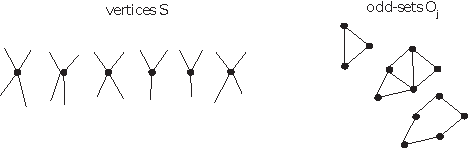
\includegraphics[width=0.8\textwidth]{figures/oddset.pdf}
	\end{figure}
}

%---------------------slide--------------------%
\frame
{
	\frametitle{Matching-duality theorem}
	
	\begin{block}{General K\"{o}nig theorem}
		If $M$ is a maximum matching and $C$ is a minimum odd-set cover then
		\begin{center}
		$|M| = capacity(C)$
		\end{center}
	\end{block}
	
	\begin{itemize}
	{
		\item Proof:
		
		\bigskip
		Edges of $M$ are covered by either $S$ or $O_{j}$. Each vertex of $S$ can cover at most one edge in the matching, and $O_{j}$ can cover at most $\frac{|O| - 1}{2}$ edges and leave one vertex exposed. Therefore, $|M| \leq capacity(C)$.
	}
	\end{itemize}
}

%---------------------slide--------------------%
\frame
{
	\frametitle{Matching-duality theorem}
	
	\begin{itemize}
	{
		\item Proof:
		
		\bigskip
		
		Then we have only to prove the existence of an odd set cover and a matching for which the numbers are equal.

		\bigskip
				
		For a pertect matching $M$ with no exposed vertices, the odd set cover consists of two sets. One is a single vertex, one consists of other vertices.
		
		\bigskip
		
		\begin{center}
		\begin{tikzpicture}
			\tikzstyle{Flower}	= [circle, fill=white, minimum size=4mm, inner sep=0pt]
			\tikzstyle{Vertex} 	= [circle, draw, solid,  fill=white, minimum size=4mm, inner sep=0pt]
			\tikzstyle{OUT}		= [fill = green, opacity = 0.5]
			\tikzstyle{IN}		= [fill = red, opacity = 0.5]
			\tikzstyle{Exposed}	= [dashed, OUT]
			\tikzstyle{MC}		= [very thick, blue]
			\tikzstyle{NM}		= [gray]
			
			\node (v1) at (0.0, 1.0) [Vertex][IN] {$1$};
			\node (v2) at (1.0, 1.0) [Vertex][OUT] {$2$};
			\node (v3) at (2.0, 1.0) [Vertex][OUT] {$3$};
			\node (v4) at (0.0, 0.0) [Vertex][OUT] {$4$};
			\node (v5) at (1.0, 0.0) [Vertex][OUT] {$5$};
			\node (v6) at (2.0, 0.0) [Vertex][OUT] {$6$};
			
			\draw [-] (v1) to (v4) [MC];
			\draw [-] (v2) to (v5) [MC];
			\draw [-] (v3) to (v6) [MC];
		\end{tikzpicture}
		\end{center}
		
	}
	\end{itemize}
}

%---------------------slide--------------------%
\frame
{
	\frametitle{Matching-duality theorem}
	
	\begin{itemize}
	{
		\item Proof:

		\bigskip
				
		For a graph which has a matching with one exposed vertices, the odd set cover consists of one set, that is the set of all the vertices.
		
		\bigskip
		
		\begin{center}
		\begin{tikzpicture}
			\tikzstyle{Flower}	= [circle, fill=white, minimum size=4mm, inner sep=0pt]
			\tikzstyle{Vertex} 	= [circle, draw, solid,  fill=white, minimum size=4mm, inner sep=0pt]
			\tikzstyle{OUT}		= [fill = green, opacity = 0.5]
			\tikzstyle{IN}		= [fill = red, opacity = 0.5]
			\tikzstyle{Exposed}	= [dashed, OUT]
			\tikzstyle{MC}		= [very thick, blue]
			\tikzstyle{NM}		= [gray]
			
			\node (v1) at (0.0, 1.0) [Vertex][Exposed][IN] {$1$};
			\node (v2) at (1.0, 1.0) [Vertex][IN] {$2$};
			\node (v3) at (2.0, 1.0) [Vertex][IN] {$3$};
			\node (v5) at (1.0, 0.0) [Vertex][IN] {$5$};
			\node (v6) at (2.0, 0.0) [Vertex][IN] {$6$};
			
			\draw [-] (v2) to (v5) [MC];
			\draw [-] (v3) to (v6) [MC];
		\end{tikzpicture}
		\end{center}
		
	}
	\end{itemize}
}

%---------------------slide--------------------%
\frame
{
	\frametitle{Matching-duality theorem}
	
	\begin{itemize}
	{
		\item Proof:

		\bigskip
				
		For a graph with more than one exposed vertex, if we run the blossom algorithm from an exposed vertex, we get an alternating tree.
		
		\bigskip
		
		\begin{center}
		\begin{tikzpicture}
			\tikzstyle{Flower}	= [circle, fill=white, minimum size=4mm, inner sep=0pt]
			\tikzstyle{Vertex} 	= [circle, draw, solid,  fill=white, minimum size=4mm, inner sep=0pt]
			\tikzstyle{OUT}		= [fill = green, opacity = 0.5]
			\tikzstyle{IN}		= [fill = red, opacity = 0.5]
			\tikzstyle{Exposed}	= [dashed]
			\tikzstyle{MC}		= [very thick, red]
			\tikzstyle{NM}		= [gray]
			
			\node (v1) at (1.0, 0) [Vertex] {};
			\node (v2) at (2.0, 0) [Vertex] {};
			\node (v3) at (3.0, 0) [Vertex] {};
			\node (v4) at (4.0, 0) [Vertex] {};
			\node (v5) at (5.0, 0) [Vertex] {};
			\node (v6) at (6.0, 0) [Vertex][Exposed]  {};
			\node (v7) at (1.0, -1) [Vertex] {};
			
			\draw [-] (v1) to (v2) [NM];
			\draw [-] (v2) to (v3) [MC];
			\draw [-] (v3) to (v4) [NM];
			\draw [-] (v4) to (v5) [MC];
			\draw [-] (v5) to (v6) [NM];
			\draw [-] (v1) to (v7) [MC];
			\draw [-] (v2) to (v7) [NM];
			\draw [-] (v5) to (5, 1) [NM];
			\draw [-] (v5) to (5, -1) [NM];
			
			\draw (v6) -- (v5) -- (v4) -- (v3) -- (v2) -- (v1) -- (v7) -- (v2) [line width=10pt, red, opacity=0.3];
		\end{tikzpicture}
		\end{center}
		
	}
	\end{itemize}
}

%---------------------slide--------------------%
\frame
{
	\frametitle{Matching-duality theorem}
	
	\begin{itemize}
	{
		\item Proof:

		\bigskip
				
		The odd set cover for the alternating tree $J$ consists of the sets of blossoms, and all the odd nodes as single vertex sets. And its capacity is equal to the size of the matching on $J$.
		
		\bigskip
		
		\begin{center}
		\begin{tikzpicture}
			\tikzstyle{Flower}	= [circle, fill=white, minimum size=4mm, inner sep=0pt]
			\tikzstyle{Vertex} 	= [circle, draw, solid,  fill=white, minimum size=4mm, inner sep=0pt]
			\tikzstyle{C1}		= [fill = green, opacity = 0.5]
			\tikzstyle{C2}		= [fill = blue, opacity = 0.5]
			\tikzstyle{Exposed}	= [dashed]
			\tikzstyle{MC}		= [very thick, red]
			\tikzstyle{NM}		= [gray]
			
			\node (v1) at (1.0, 0) [Vertex][C1] {};
			\node (v2) at (2.0, 0) [Vertex][C1] {};
			\node (v3) at (3.0, 0) [Vertex][C2] {};
			\node (v4) at (4.0, 0) [Vertex] {};
			\node (v5) at (5.0, 0) [Vertex][C2] {};
			\node (v6) at (6.0, 0) [Vertex][Exposed]  {};
			\node (v7) at (1.0, -1) [Vertex][C1] {};
			
			\draw [-] (v1) to (v2) [NM];
			\draw [-] (v2) to (v3) [MC];
			\draw [-] (v3) to (v4) [NM];
			\draw [-] (v4) to (v5) [MC];
			\draw [-] (v5) to (v6) [NM];
			\draw [-] (v1) to (v7) [MC];
			\draw [-] (v2) to (v7) [NM];
			\draw [-] (v5) to (5, 1) [NM];
			\draw [-] (v5) to (5, -1) [NM];
			
			\draw (v6) -- (v5) -- (v4) -- (v3) -- (v2) -- (v1) -- (v7) -- (v2) [line width=10pt, red, opacity=0.3];
		\end{tikzpicture}
		\end{center}
		
	}
	\end{itemize}
}

%---------------------slide--------------------%
\frame
{
	\frametitle{Matching-duality theorem}
	
	\begin{itemize}
	{
		\item Proof:

		\bigskip
				
		For the other components of the graph $G-J$, the number of exposed vertex is reduced by one. If we assume $|M_{G-J}|=capacity(C_{G-J})$, we can prove the theorem by induction. 
		
		\bigskip
		
		\begin{center}
		\begin{tikzpicture}
			\tikzstyle{Flower}	= [circle, fill=white, minimum size=4mm, inner sep=0pt]
			\tikzstyle{Vertex} 	= [circle, draw, solid,  fill=white, minimum size=4mm, inner sep=0pt]
			\tikzstyle{C1}		= [fill = green, opacity = 0.5]
			\tikzstyle{C2}		= [fill = blue, opacity = 0.5]
			\tikzstyle{Exposed}	= [dashed]
			\tikzstyle{MC}		= [very thick, red]
			\tikzstyle{NM}		= [gray]
			
			\node (v1) at (1.0, 0) [Vertex][C1] {};
			\node (v2) at (2.0, 0) [Vertex][C1] {};
			\node (v3) at (3.0, 0) [Vertex][C2] {};
			\node (v4) at (4.0, 0) [Vertex] {};
			\node (v5) at (5.0, 0) [Vertex][C2] {};
			\node (v6) at (6.0, 0) [Vertex][Exposed]  {};
			\node (v7) at (1.0, -1) [Vertex][C1] {};
			
			\draw [-] (v1) to (v2) [NM];
			\draw [-] (v2) to (v3) [MC];
			\draw [-] (v3) to (v4) [NM];
			\draw [-] (v4) to (v5) [MC];
			\draw [-] (v5) to (v6) [NM];
			\draw [-] (v1) to (v7) [MC];
			\draw [-] (v2) to (v7) [NM];
			\draw [-] (v5) to (5, 1) [NM];
			\draw [-] (v5) to (5, -1) [NM];
			
			\draw (v6) -- (v5) -- (v4) -- (v3) -- (v2) -- (v1) -- (v7) -- (v2) [line width=10pt, red, opacity=0.3];
		\end{tikzpicture}
		\end{center}
		
	}
	\end{itemize}
}

\frame
{
	\frametitle{Summary}
	\begin{itemize}
		\item<1-> We have found the dual problem to maximum matching on general graphs!
		\item<2-> Although maximum matching is an integer programming problem, which is inherently intractable, Edmonds proved in another paper that the optimal value of this integer programming is equal to the optimal value of the corresponding linear programming problem, if we relax the integral constraints. But it is beyond the scope of this talk.
	\end{itemize}
}

\frame
{
	\frametitle{Conclusion}
	\begin{itemize}
		\item<1-> We have defined what an efficient algorithm is.
		\item<2-> We have extended the algorithm for finding maximum matching on bipartite graph to the general graph, which has polynomial running time guarantee.
		\item<3-> We have generalized K\"{o}nig theorem to general graph which is mathematically elegant.
	\end{itemize}
}

{
\usebackgroundtemplate{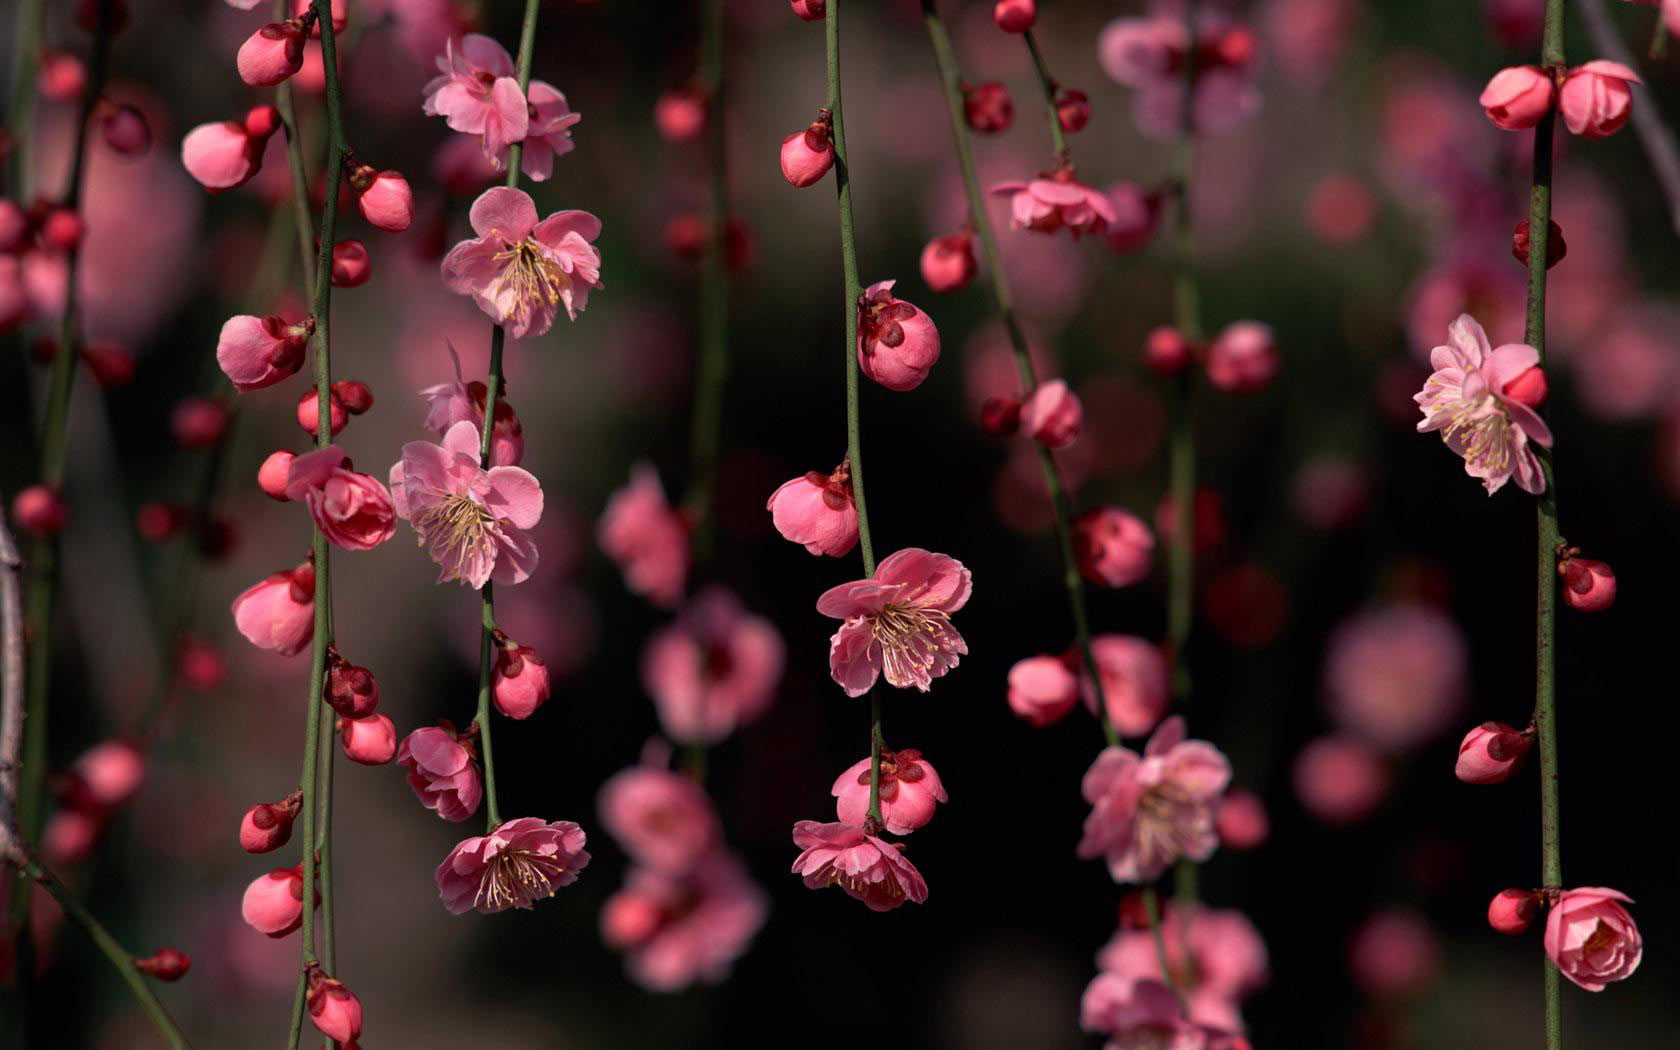
\includegraphics[width=\paperwidth, height=\paperheight]{figures/flower}}
\begin{frame}
	\begin{textblock*}{\paperwidth}[0,0](0cm,3cm)
		\begin{center}
			\usebeamercolor[fg]{title}
			\textbf{\huge {Thank you! \&\& Questions?}}
		\end{center}
		\usebeamercolor[fg]{normal text}
	\end{textblock*}
\end{frame}
}

%---------------------slide--------------------%
\frame
{
	\frametitle{Appendix}
	
	\begin{block}{Lemma 1}
	If $G/B$ contains an augmenting path $P$ starting at $r$ (or the pseudo node containing $r$), w.r.t. the matching $M/B$, then $G$ contains an augmenting path starting at $r$ w.r.t. matching $M$.
	\end{block}
	
}

%---------------------slide--------------------%
\frame
{
	\frametitle{Proof of Lemma 1}
	
	\textbf{Proof:}
	
	\bigskip
	
	If $P$ does not contain the pseudo node $b$, it is also augmenting path in $G$.
	
	\textbf{Case 1: non-empty stem}
	
	\begin{itemize}
		\item Next suppose that the stem is non-empty.
	\end{itemize}

	\begin{center}
	\begin{tikzpicture}
		\tikzstyle{Flower}	= [circle, fill=white, minimum size=4mm, inner sep=0pt]
		\tikzstyle{Vertex} 	= [circle, draw, solid,  fill=white, minimum size=4mm, inner sep=0pt]
		\tikzstyle{OUT}		= [fill = white]
		\tikzstyle{IN}		= [fill = black]
		\tikzstyle{Exposed}	= [dashed, OUT]
		\tikzstyle{MC}		= [very thick, blue]
		\tikzstyle{NM}		= [gray]
		
		\node (v1) at (0, 0) [Vertex][Exposed] {$r$};
		\node (v2) at (1, 0) [Vertex] {$i$};
		\node (v3) at (2, 0) [Flower][label=above:b] {};
			%\myflower.apply(6.0, 5.0, 0.3)	
				\pgfplothandlerlineto
				\pgfplotfunction{\x}{0, 3, ..., 540}{
					\pgfpointxy     
					{-0.2 * cos(\x) * sin(5 / 3 * \x) + 2}
					{-0.2 * sin(\x) * sin(5 / 3 * \x) + 0}
				}
				\pgfusepath{stroke}
		\node (v4) at (3, 0) [Vertex] {$j$};
		\node (v5) at (4, 0) [Vertex][Exposed] {$q$};
		
		\draw [-] (v1) to (v2) [NM][dashed];
		\draw [-] (v2) to (v3) [MC];
		\draw [-] (v3) to (v4) [NM];
		\draw [-] (v4) to (v5) [NM][dashed];
		
		\node at (0.5, 0) [label=above:$P_{1}$] {};
		\node at (3.5, 0) [label=above:$P_{2}$] {};
		
		%\draw (v1) -- (v2) -- (v3) -- (v4) -- (v5) -- (v7) [line width=10pt, red, opacity=0.3];
	\end{tikzpicture}
	\end{center}
}

%---------------------slide--------------------%
\frame
{
	\frametitle{Proof of Lemma 1}
	
	\begin{center}
	\begin{tikzpicture}
		\tikzstyle{Flower}	= [circle, fill=white, minimum size=4mm, inner sep=0pt]
		\tikzstyle{Vertex} 	= [circle, draw, solid,  fill=white, minimum size=4mm, inner sep=0pt]
		\tikzstyle{OUT}		= [fill = white]
		\tikzstyle{IN}		= [fill = black]
		\tikzstyle{Exposed}	= [dashed, OUT]
		\tikzstyle{MC}		= [very thick, blue]
		\tikzstyle{NM}		= [gray]
		
		\node (v1) at (0, 0) [Vertex][Exposed] {$r$};
		\node (v2) at (1, 0) [Vertex] {$i$};
		\node (v3) at (2, 0) [Flower][label=above:b] {};
			%\myflower.apply(6.0, 5.0, 0.3)	
				\pgfplothandlerlineto
				\pgfplotfunction{\x}{0, 3, ..., 540}{
					\pgfpointxy     
					{-0.2 * cos(\x) * sin(5 / 3 * \x) + 2}
					{-0.2 * sin(\x) * sin(5 / 3 * \x) + 0}
				}
				\pgfusepath{stroke}
		\node (v4) at (3, 0) [Vertex] {$j$};
		\node (v5) at (4, 0) [Vertex][Exposed] {$q$};
		
		\draw [-] (v1) to (v2) [NM][dashed];
		\draw [-] (v2) to (v3) [MC];
		\draw [-] (v3) to (v4) [NM];
		\draw [-] (v4) to (v5) [NM][dashed];
		
		\node at (0.5, 0) [label=above:$P_{1}$] {};
		\node at (3.5, 0) [label=above:$P_{2}$] {};
		
		%\draw (v1) -- (v2) -- (v3) -- (v4) -- (v5) -- (v7) [line width=10pt, red, opacity=0.3];
	\end{tikzpicture}
	\end{center}
	
	\begin{itemize}
		\item After the expansion, $j$ must be incident to some node in the blossom. Let this node be $k$.
		\item If $k \neq w$, there is an alternating path $P_{2}$ from $w$ to $k$ that ends in a matching edge.
		\item $P_{1}$ + $(i,w)$ + $P_{2}$ + $(k,j)$ + $P_{3}$ is an augmenting path.
	\end{itemize}

	\begin{center}
	\begin{tikzpicture}
		\tikzstyle{Flower}	= [circle, fill=white, minimum size=4mm, inner sep=0pt]
		\tikzstyle{Vertex} 	= [circle, draw, solid,  fill=white, minimum size=4mm, inner sep=0pt]
		\tikzstyle{OUT}		= [fill = white]
		\tikzstyle{IN}		= [fill = black]
		\tikzstyle{Exposed}	= [dashed, OUT]
		\tikzstyle{MC}		= [very thick, blue]
		\tikzstyle{NM}		= [gray]
		
		\node (v1) at (0, 0) [Vertex][Exposed] {$r$};
		\node (v2) at (1, 0) [Vertex] {$i$};
		\node (v3) at (2, 0) [Vertex]{$w$};
		\node (v4) at (3, 1) [Vertex] {};
		\node (v5) at (4, 1) [Vertex] {};
		\node (v6) at (5, 1) [Vertex]{$k$};
		\node (v7) at (5, -1) [Vertex]{};
		\node (v8) at (4, -1) [Vertex]{};
		\node (v9) at (3, -1) [Vertex]{};
		\node (v10) at (6, 1) [Vertex]{$j$};
		\node (v11) at (7, 1) [Vertex][Exposed] {$q$};
		
		\draw [-] (v1) to (v2) [NM][dashed];
		\draw [-] (v2) to (v3) [MC];
		\draw [-] (v3) to (v4) [NM];
		\draw [-] (v4) to (v5) [MC];
		\draw [-] (v5) to (v6) [NM];
		\draw [-] (v6) to (v7) [MC];
		\draw [-] (v7) to (v8) [NM];
		\draw [-] (v8) to (v9) [MC];
		\draw [-] (v9) to (v3) [NM];
		\draw [-] (v6) to (v10) [NM];
		\draw [-] (v10) to (v11) [NM][dashed];
		
		\node at (0.5, 0) [label=above:$P_{1}$] {};
		\node at (4, -1) [label=above:$P_{2}$] {};
		\node at (6.5, 1) [label=above:$P_{3}$] {};
		
		\draw (v1) -- (v2) -- (v3) -- (v9) -- (v8) -- (v7) -- (v6) -- (v10) -- (v11)[line width=10pt, red, opacity=0.3];
	\end{tikzpicture}
	\end{center}
}

%---------------------slide--------------------%
\frame
{
	\frametitle{Proof of Lemma 1}
	
	\begin{itemize}
		\item if $k=w$, then $P_{1}$ + $(i,w)$ + $(w,j)$ + $P_{3}$ is an augmenting path.
	\end{itemize}

	\begin{center}
	\begin{tikzpicture}
		\tikzstyle{Flower}	= [circle, fill=white, minimum size=4mm, inner sep=0pt]
		\tikzstyle{Vertex} 	= [circle, draw, solid,  fill=white, minimum size=4mm, inner sep=0pt]
		\tikzstyle{OUT}		= [fill = white]
		\tikzstyle{IN}		= [fill = black]
		\tikzstyle{Exposed}	= [dashed, OUT]
		\tikzstyle{MC}		= [very thick, blue]
		\tikzstyle{NM}		= [gray]
		
		\node (v1) at (0, 0) [Vertex][Exposed] {$r$};
		\node (v2) at (1, 0) [Vertex] {$i$};
		\node (v3) at (2, 0) [Vertex][label=above:$k$]{$w$};
		\node (v4) at (3, -1) [Vertex] {};
		\node (v5) at (3, -2) [Vertex] {};
		\node (v6) at (3, -3) [Vertex]{};
		\node (v7) at (1, -3) [Vertex]{};
		\node (v8) at (1, -2) [Vertex]{};
		\node (v9) at (1, -1) [Vertex]{};
		\node (v10) at (3, 0) [Vertex]{$j$};
		\node (v11) at (4, 0) [Vertex][Exposed] {$q$};
		
		\draw [-] (v1) to (v2) [NM][dashed];
		\draw [-] (v2) to (v3) [MC];
		\draw [-] (v3) to (v4) [NM];
		\draw [-] (v4) to (v5) [MC];
		\draw [-] (v5) to (v6) [NM];
		\draw [-] (v6) to (v7) [MC];
		\draw [-] (v7) to (v8) [NM];
		\draw [-] (v8) to (v9) [MC];
		\draw [-] (v9) to (v3) [NM];
		\draw [-] (v3) to (v10) [NM];
		\draw [-] (v10) to (v11) [NM][dashed];
		
		\node at (0.5, 0) [label=above:$P_{1}$] {};
		\node at (3.5, 0) [label=above:$P_{3}$] {};
		
		\draw (v1) -- (v2) -- (v3) -- (v10) -- (v11)[line width=10pt, red, opacity=0.3];
	\end{tikzpicture}
	\end{center}
}

%---------------------slide--------------------%
\frame
{
	\frametitle{Proof of Lemma 1}
	
	\textbf{Proof:}
	
	\bigskip
	
	\textbf{Case 2: empty stem}
	
	\begin{itemize}
		\item If the stem is empty then after expanding the blossom, $w=r$.
	\end{itemize}

	\begin{center}
	\begin{tikzpicture}
		\tikzstyle{Flower}	= [circle, fill=white, minimum size=4mm, inner sep=0pt]
		\tikzstyle{Vertex} 	= [circle, draw, solid,  fill=white, minimum size=4mm, inner sep=0pt]
		\tikzstyle{OUT}		= [fill = white]
		\tikzstyle{IN}		= [fill = black]
		\tikzstyle{Exposed}	= [dashed, OUT]
		\tikzstyle{MC}		= [very thick, blue]
		\tikzstyle{NM}		= [gray]
		
		\node (v1) at (1, 0) [Flower][label=above:b] {};
			%\myflower.apply(6.0, 5.0, 0.3)	
				\pgfplothandlerlineto
				\pgfplotfunction{\x}{0, 3, ..., 540}{
					\pgfpointxy     
					{-0.2 * cos(\x) * sin(5 / 3 * \x) + 1}
					{-0.2 * sin(\x) * sin(5 / 3 * \x) + 0}
				}
				\pgfusepath{stroke}
		\node (v2) at (2, 0) [Vertex] {$j$};
		\node (v3) at (3, 0) [Vertex][Exposed] {$q$};
		
		\draw [-] (v1) to (v2) [NM];
		\draw [-] (v2) to (v3) [NM][dashed];
		
		\node at (2.5, 0) [label=above:$P_{3}$] {};
		
		%\draw (v1) -- (v2) -- (v3) -- (v4) -- (v5) -- (v7) -- (v1)[line width=10pt, red, opacity=0.3];
	\end{tikzpicture}
	\end{center}
	
	\begin{center}
	\begin{tikzpicture}
		\tikzstyle{Flower}	= [circle, fill=white, minimum size=4mm, inner sep=0pt]
		\tikzstyle{Vertex} 	= [circle, draw, solid,  fill=white, minimum size=4mm, inner sep=0pt]
		\tikzstyle{OUT}		= [fill = white]
		\tikzstyle{IN}		= [fill = black]
		\tikzstyle{Exposed}	= [dashed, OUT]
		\tikzstyle{MC}		= [very thick, blue]
		\tikzstyle{NM}		= [gray]
		
		\node (v1) at (1, 0) [Vertex][Exposed][label=above:$r$] {$w$};
		\node (v2) at (2, 1) [Vertex] {};
		\node (v3) at (3, 1) [Vertex] {};
		\node (v4) at (4, 1) [Vertex] {$k$};
		\node (v5) at (4, -1) [Vertex] {};
		\node (v6) at (3, -1) [Vertex] {};
		\node (v7) at (2, -1) [Vertex] {};
		\node (v8) at (5, 1) [Vertex] {$j$};
		\node (v9) at (6, 1) [Vertex] {$q$};
		
		\draw [-] (v1) to (v2) [NM];
		\draw [-] (v2) to (v3) [MC];
		\draw [-] (v3) to (v4) [NM];
		\draw [-] (v4) to (v5) [MC];
		\draw [-] (v5) to (v6) [NM];
		\draw [-] (v6) to (v7) [MC];
		\draw [-] (v7) to (v1) [NM];
		\draw [-] (v4) to (v8) [NM];
		\draw [-] (v8) to (v9) [NM][dashed];
		
		\node at (3, -1) [label=above:$P_{2}$] {};
		\node at (5.5, 1) [label=above:$P_{3}$] {};
		
		\draw (v1) -- (v7) -- (v6) -- (v5) -- (v4) -- (v8) -- (v9) [line width=10pt, red, opacity=0.3];
	\end{tikzpicture}
	\end{center}
	
	\begin{itemize}
		\item The path $r$ + $P_{2}$ + $(k,j)$ + $P_{3}$ is an augmenting path.
	\end{itemize}
}

%---------------------slide--------------------%
\frame
{
	\frametitle{Proof of Lemma 2}
	
	\begin{block}{Lemma 2}
	If $G$ contains an augmenting path $P$ from $r$ to $q$ w.r.t. matching $M$ then $G/B$ contains an augmenting path from $r$ (or the pseudo node containing $r$) to $q$ w.r.t. the matching $M/B$.
	\end{block}
	
	\textbf{Proof:}
	
	\bigskip
	
	\begin{itemize}
		\item If $P$ does not contain a node from $B$ there is nothing to prove.
		\item We can assume that $r$ and $q$ are the only exposed nodes in $G$.
	\end{itemize}
}

%---------------------slide--------------------%
\frame
{
	\frametitle{Proof of Lemma 2}
	
	\textbf{Case 1: empty stem}
	
	\begin{itemize}
		\item Let $i$ be the last node on the path $P$ that is part of the blossom.
		\item $P$ is of the form $P_{1}$ + $(i,j)$ + $P_{2}$, for some node $j$ and $(i, j)$ is unmatched.
		\item $(b,j)$ + $P_{2}$ is an augmenting path in the contracted graph.
	\end{itemize}

	\begin{center}
	\begin{tikzpicture}
		\tikzstyle{Flower}	= [circle, fill=white, minimum size=4mm, inner sep=0pt]
		\tikzstyle{Vertex} 	= [circle, draw, solid,  fill=white, minimum size=4mm, inner sep=0pt]
		\tikzstyle{OUT}		= [fill = white]
		\tikzstyle{IN}		= [fill = black]
		\tikzstyle{Exposed}	= [dashed, OUT]
		\tikzstyle{MC}		= [very thick, blue]
		\tikzstyle{NM}		= [gray]
		
		\node (v1) at (1, 0) [Vertex][Exposed]{$w$};
		\node (v2) at (2, 1) [Vertex] {};
		\node (v3) at (3, 1) [Vertex] {};
		\node (v4) at (4, 1) [Vertex] {};
		\node (v5) at (5, 1) [Vertex] {};
		\node (v6) at (6, 1) [Vertex] {};
		\node (v7) at (6, -1) [Vertex] {};
		\node (v8) at (5, -1) [Vertex] {};
		\node (v9) at (4, -1) [Vertex] {$i$};
		\node (v10) at (3, -1) [Vertex] {};
		\node (v11) at (2, -1) [Vertex] {};
		\node (v12) at (4.5, -2) [Vertex] {$j$};
		\node (v13) at (5.5, -2) [Vertex][Exposed] {$q$};
		
		\draw [-] (v1) to (v2) [NM];
		\draw [-] (v2) to (v3) [MC];
		\draw [-] (v3) to (v4) [NM];
		\draw [-] (v4) to (v5) [MC];
		\draw [-] (v5) to (v6) [NM];
		\draw [-] (v6) to (v7) [MC];
		\draw [-] (v7) to (v8) [NM];
		\draw [-] (v8) to (v9) [MC];
		\draw [-] (v9) to (v10) [NM];
		\draw [-] (v10) to (v11) [MC];
		\draw [-] (v11) to (v1) [NM];
		\draw [-] (v9) to (v12) [NM];
		\draw [-] (v12) to (v13) [NM][dashed];
		
		\node at (6, 0) [label=right:$P_{1}$] {};
		\node at (5, -2) [label=above:$P_{2}$] {};
		
		\draw (v1) -- (v2) -- (v3) -- (v4) -- (v5) -- (v6) -- (v7) -- (v8) -- (v9) -- (v12) -- (v13)[line width=10pt, red, opacity=0.3];
	\end{tikzpicture}
	\end{center}
	
	\begin{center}
	\begin{tikzpicture}
		\tikzstyle{Flower}	= [circle, fill=white, minimum size=4mm, inner sep=0pt]
		\tikzstyle{Vertex} 	= [circle, draw, solid,  fill=white, minimum size=4mm, inner sep=0pt]
		\tikzstyle{OUT}		= [fill = white]
		\tikzstyle{IN}		= [fill = black]
		\tikzstyle{Exposed}	= [dashed, OUT]
		\tikzstyle{MC}		= [very thick, blue]
		\tikzstyle{NM}		= [gray]
		
		\node (v1) at (1, 0) [Flower][label=above:b] {};
			%\myflower.apply(6.0, 5.0, 0.3)	
				\pgfplothandlerlineto
				\pgfplotfunction{\x}{0, 3, ..., 540}{
					\pgfpointxy     
					{-0.2 * cos(\x) * sin(5 / 3 * \x) + 1}
					{-0.2 * sin(\x) * sin(5 / 3 * \x) + 0}
				}
				\pgfusepath{stroke}
		\node (v2) at (2, 0) [Vertex] {$j$};
		\node (v3) at (3, 0) [Vertex][Exposed] {$q$};
		
		\draw [-] (v1) to (v2) [NM];
		\draw [-] (v2) to (v3) [NM][dashed];

		\node at (2.5, 0) [label=above:$P_{2}$] {};
		
		\draw (v1) -- (v2) -- (v3)[line width=10pt, red, opacity=0.3];
	\end{tikzpicture}
	\end{center}
}

%---------------------slide--------------------%
\frame
{
	\frametitle{Proof of Lemma 2}
	
	\textbf{Case 2: non-empty stem}
	
	\begin{itemize}
		\item Let $P_{3}$ be alternating path from $r$ to $w$. Define $M_{+}=M \oplus P_{3}$.
	\end{itemize}
	
	\begin{center}
	\begin{tikzpicture}[scale=0.7]
		\tikzstyle{Flower}	= [circle, fill=white, minimum size=4mm, inner sep=0pt]
		\tikzstyle{Vertex} 	= [circle, draw, solid,  fill=white, minimum size=4mm, inner sep=0pt]
		\tikzstyle{OUT}		= [fill = white]
		\tikzstyle{IN}		= [fill = black]
		\tikzstyle{Exposed}	= [dashed, OUT]
		\tikzstyle{MC}		= [very thick, blue]
		\tikzstyle{NM}		= [gray]
		
		\node (v0) at (-1, 0) [Vertex][Exposed] {$r$};
		\node (v1) at (0, 0) [Vertex]{};
		\node (v2) at (1, 0) [Vertex] {$i$};
		\node (v3) at (2, 0) [Vertex]{$w$};
		\node (v4) at (3, 1) [Vertex] {};
		\node (v5) at (4, 1) [Vertex] {};
		\node (v6) at (5, 1) [Vertex]{$k$};
		\node (v7) at (5, -1) [Vertex]{};
		\node (v8) at (4, -1) [Vertex]{};
		\node (v9) at (3, -1) [Vertex]{};
		\node (v10) at (6, 1) [Vertex]{$j$};
		\node (v11) at (7, 1) [Vertex][Exposed] {$q$};
		
		\draw [-] (v0) to (v1) [NM][dashed];
		\draw [-] (v1) to (v2) [NM];
		\draw [-] (v2) to (v3) [MC];
		\draw [-] (v3) to (v4) [NM];
		\draw [-] (v4) to (v5) [MC];
		\draw [-] (v5) to (v6) [NM];
		\draw [-] (v6) to (v7) [MC];
		\draw [-] (v7) to (v8) [NM];
		\draw [-] (v8) to (v9) [MC];
		\draw [-] (v9) to (v3) [NM];
		\draw [-] (v6) to (v10) [NM];
		\draw [-] (v10) to (v11) [NM][dashed];
		
		\node at (0.5, 0) [label=above:$P_{3}$] {};
		
		\draw (v0) -- (v1) -- (v2) -- (v3)[line width=10pt, blue, opacity=0.3];
	\end{tikzpicture}
	\end{center}
}

%---------------------slide--------------------%
\frame
{
	\frametitle{Proof of Lemma 2}
	
	\textbf{Case 2: non-empty stem}
	
	\begin{itemize}
		\item In $M_{+}$, $r$ is matched and $w$ is unmatched.
		\item $G$ must contain an augmenting path w.r.t. matching $M_{+}$, since $M$ and $M_{+}$ have same cardinality.
		\item This path must go between $w$ and $q$ as these are the only unmatched vertices w.r.t. $M_{+}$.
	\end{itemize}
	
	\begin{center}
	\begin{tikzpicture}[scale=0.7]
		\tikzstyle{Flower}	= [circle, fill=white, minimum size=4mm, inner sep=0pt]
		\tikzstyle{Vertex} 	= [circle, draw, solid,  fill=white, minimum size=4mm, inner sep=0pt]
		\tikzstyle{OUT}		= [fill = white]
		\tikzstyle{IN}		= [fill = black]
		\tikzstyle{Exposed}	= [dashed, OUT]
		\tikzstyle{MC}		= [very thick, blue]
		\tikzstyle{NM}		= [gray]
		
		\node (v0) at (-1, 0) [Vertex] {$r$};
		\node (v1) at (0, 0) [Vertex]{};
		\node (v2) at (1, 0) [Vertex] {$i$};
		\node (v3) at (2, 0) [Vertex][Exposed]{$w$};
		\node (v4) at (3, 1) [Vertex] {};
		\node (v5) at (4, 1) [Vertex] {};
		\node (v6) at (5, 1) [Vertex]{$k$};
		\node (v7) at (5, -1) [Vertex]{};
		\node (v8) at (4, -1) [Vertex]{};
		\node (v9) at (3, -1) [Vertex]{};
		\node (v10) at (6, 1) [Vertex]{$j$};
		\node (v11) at (7, 1) [Vertex][Exposed] {$q$};
		
		\draw [-] (v0) to (v1) [NM][dashed];
		\draw [-] (v1) to (v2) [MC];
		\draw [-] (v2) to (v3) [NM];
		\draw [-] (v3) to (v4) [NM];
		\draw [-] (v4) to (v5) [MC];
		\draw [-] (v5) to (v6) [NM];
		\draw [-] (v6) to (v7) [MC];
		\draw [-] (v7) to (v8) [NM];
		\draw [-] (v8) to (v9) [MC];
		\draw [-] (v9) to (v3) [NM];
		\draw [-] (v6) to (v10) [NM];
		\draw [-] (v10) to (v11) [NM][dashed];
		
		\node at (0.5, 0) [label=above:$P_{3}$] {};
		
		%\draw (v3) -- (v9) -- (v8) -- (v7) -- (v6) -- (v10) -- (v11)[line width=10pt, red, opacity=0.3];
	\end{tikzpicture}
	\end{center}
	
}

%---------------------slide--------------------%
\frame
{
	\frametitle{Proof of Lemma 2}
	
	\textbf{Case 2: non-empty stem}
	
	\begin{itemize}
		\item For $M_{+}/B$ the blossom has an empty stem. Case 1 applies.
		\item $G/B$ has an augmenting path w.r.t. $M_{+}/B$. It must also have an augmenting path w.r.t. $M/B$, as both matchings have the same cardinality.
		\item This path must go between $r$ and $q$, since they are the only exposed nodes.
	\end{itemize}
	
	\begin{center}
	\begin{tikzpicture}[scale=0.7]
		\tikzstyle{Flower}	= [circle, fill=white, minimum size=4mm, inner sep=0pt]
		\tikzstyle{Vertex} 	= [circle, draw, solid,  fill=white, minimum size=4mm, inner sep=0pt]
		\tikzstyle{OUT}		= [fill = white]
		\tikzstyle{IN}		= [fill = black]
		\tikzstyle{Exposed}	= [dashed, OUT]
		\tikzstyle{MC}		= [very thick, blue]
		\tikzstyle{NM}		= [gray]
		
		\node (v3) at (2, 0) [Vertex][Exposed]{$w$};
		\node (v4) at (3, 1) [Vertex] {};
		\node (v5) at (4, 1) [Vertex] {};
		\node (v6) at (5, 1) [Vertex]{$k$};
		\node (v7) at (5, -1) [Vertex]{};
		\node (v8) at (4, -1) [Vertex]{};
		\node (v9) at (3, -1) [Vertex]{};
		\node (v10) at (6, 1) [Vertex]{$j$};
		\node (v11) at (7, 1) [Vertex][Exposed] {$q$};
		
		\draw [-] (v3) to (v4) [NM];
		\draw [-] (v4) to (v5) [MC];
		\draw [-] (v5) to (v6) [NM];
		\draw [-] (v6) to (v7) [MC];
		\draw [-] (v7) to (v8) [NM];
		\draw [-] (v8) to (v9) [MC];
		\draw [-] (v9) to (v3) [NM];
		\draw [-] (v6) to (v10) [NM];
		\draw [-] (v10) to (v11) [NM][dashed];
				
		\draw (v3) -- (v9) -- (v8) -- (v7) -- (v6) -- (v10) -- (v11)[line width=10pt, red, opacity=0.3];
	\end{tikzpicture}
	\end{center}
	
	\begin{center}
	\begin{tikzpicture}
		\tikzstyle{Flower}	= [circle, fill=white, minimum size=4mm, inner sep=0pt]
		\tikzstyle{Vertex} 	= [circle, draw, solid,  fill=white, minimum size=4mm, inner sep=0pt]
		\tikzstyle{OUT}		= [fill = white]
		\tikzstyle{IN}		= [fill = black]
		\tikzstyle{Exposed}	= [dashed, OUT]
		\tikzstyle{MC}		= [very thick, blue]
		\tikzstyle{NM}		= [gray]
		
		\node (v1) at (1, 0) [Flower][label=above:b] {};
			%\myflower.apply(6.0, 5.0, 0.3)	
				\pgfplothandlerlineto
				\pgfplotfunction{\x}{0, 3, ..., 540}{
					\pgfpointxy     
					{-0.2 * cos(\x) * sin(5 / 3 * \x) + 1}
					{-0.2 * sin(\x) * sin(5 / 3 * \x) + 0}
				}
				\pgfusepath{stroke}
		\node (v2) at (2, 0) [Vertex] {$j$};
		\node (v3) at (3, 0) [Vertex][Exposed] {$q$};
		
		\draw [-] (v1) to (v2) [NM];
		\draw [-] (v2) to (v3) [NM][dashed];

		\node at (2.5, 0) [label=above:$P_{2}$] {};
		
		\draw (v1) -- (v2) -- (v3)[line width=10pt, red, opacity=0.3];
	\end{tikzpicture}
	\end{center}
	
}

%---------------------slide--------------------%
\frame
{
	\frametitle{Reference}
		
	\begin{itemize}
		\item \url{http://wwwmayr.informatik.tu-muenchen.de/lehre/2011WS/ea/index.html.en}
		\item \url{www.cs.berkeley.edu/~karp/greatalgo/}
		\item \url{en.wikipedia.org/wiki/Edmonds's_matching_algorithm}
		\item \url{http://ilyoan.tistory.com/entry/Paths-Trees-and-Flowers-presentation}
		\item \url{http://www.slideshare.net/akhayyat/maximum-matching-in-general-graphs}
		\item \url{http://www.csie.ntnu.edu.tw/~u91029/Matching.html}
		\item \url{http://www.cse.cuhk.edu.hk/~chi/csc5160-2008/notes.html}
		\item \url{https://tkramesh.wordpress.com/2009/10/02/bipartite-matching-an-application/}
	\end{itemize}

}

\end{document}
